%!TEX TS-program = /usr/texbin/pdflatex
%!GEDIT texbin = /usr/local/texlive/current/bin/x86_64-linux/pdflatex
%
%	''Becker-Vorlage'' style LaTeX template

% 	This template is  MIT licensed, authors:
%   Jan Betzing <jan.betzing@ercis.uni-muenster.de> *corresponding author
%	Dominik Lekse <dominik@lekse.de>
%
% 	Basic file to demonstrate the usage of this LaTeX template.
% 	You can build your own paper/thesis on top of this file.
% 	Simply adjust the document class and all metadata and start working.
%
\documentclass[
  language=german, % set to english or german
  type=bachelor,% set to bachelor, master or seminar
  ngerman
]{isthesis}

% Graphics rendering using TikZ
% See: https://en.wikibooks.org/wiki/LaTeX/PGF/TikZ
\usepackage{tikz}
\usetikzlibrary{fit}
\usepackage{textcomp}
\usepackage{caption}
\usepackage{forest}
\usepackage{babel}
% Include required TikZ libraries here, some exemplary libraries are pre-included
\usetikzlibrary{calc}
\usetikzlibrary{matrix}
\usetikzlibrary{positioning}
\usetikzlibrary{shapes.geometric}
\usetikzlibrary{er}
\usepackage{cleveref}


% Import acronyms
% \newacronym[longplural={<long plural>}, shortplural={<short plural>}]{<label>}{<short>}{<long>}
% 	label = is the unique identifier and sort key for the acronym, can be the same as <short>
%	short = is the abbreviation or acronym
%	short plural (optional) = is the plural of the abbreviation or acronym
%	long = is the long form of the acronym, this will appear in the list of abbreviations
%	long plural (optional) = is the long plural form of the abbreviation or acronym

\newacronym[shortplural={KMUen}, longplural={Kleine und Mittlere Unternehmen}]{kmu}{KMU}{Kleines und Mittleres Unternehmen}
\newacronym{CD}{CD}{Corporate Design}
\newacronym{SQL}{SQL}{Structured Query Language}
\newacronym{ERCIS}{ERCIS}{European Research Center for Information Systems}
\newacronym{WWU}{WWU}{Westf\"alische Wilhelms-Universit\"at}
\newacronym{BPM}{BPM}{Business Process Management}
\newacronym{npm}{NPM}{Node Package Manager}
\newacronym{DWH}{DWH}{Data Warehouse}
\newacronym{DQM}{DQM}{Datenqualitätsmanagement}
\newacronym{OLTP}{OLTP}{Online-Transaction-Processing}
\newacronym{OLAP}{OLAP}{Online-Analytical-Processing}
\newacronym{ERM}{ERM}{Entity-Relationship-Modell}
\newacronym{CRM}{CRM}{Customer-Relationship-Management}


% Import symbols
% Syntax: <Symbol> <Label> <Name>
% The symbols are sorted by their labels
\addsymboltolist{$\Pi$}{Pi}{Projection}
\addsymboltolist{$\Join$}{Join}{Natural Join}
\addsymboltolist{$\sigma$}{Selection}{Selection}


% Document meta information
\isthesis{title={Entwicklung einer Sprache zur Modellierung von Qualitätskennzahlen für \textit{DataRocket} und deren prototypische Implementierung},
  author={Max Leonard Inden},
  author-email={max.inden@uni-muenster.de},
  author-phone={+49 178 1493411}, % Use international numbers format
  author-matriculation={409098},
  author-address={Biemsmaar 4c},
  author-zip={53343},
  author-city={Wachtberg},
  principal-supervisor={Prof.\ Dr.\ Dr.\ h.c. Dr.\ h.c. J\"org Becker}, % This has to be a professor
  associate-supervisor={Dr.\ Stefan Fleischer}, % This is your main supervisor, i.e., a post doc or PhD student
  tutor-supervisor={}, % If required, define an additional supervisor resp. tutor here
  group={Lehrstuhl für Wirtschaftsinformatik und Informationsmanagement},
  group-institute={Westfälische Wilhelms-Universität, M\"unster},
  associate-group={innoscale AG}, % When the thesis is done in cooperation with another chair, add it here
  %associate-group-institute={innoscale AG}, % add cooperating institute or university here
  seminar={Scientific Writing for Beginners}, % The title of your seminar
  submission-date={}, % !!! In  isthesis.cls ändern
  %primary-logo={}, % Uses the WWU logo by default
  %primary-logo-height={}, % Uses 16mm as default height
  secondary-logo={lib/assets/innoscale-logo}, % Logo of the secondary institution (cooperating chair/university), USES Faculty logo by default
  %secondary-logo-height={} % Uses 16mm as default height
}
\begin{document}
% Title page
\maketitle

% Quote
% You can put an optional quote page in front of your content
%\quotepage[author={Arthur C. Clarke}]{
%  Any sufficiently advanced technology is indistinguishable from magic.
%}

% Table of contents
\tableofcontents

% List of figures (if you have figures)
\listoffigures

% List of tables (if you have tables)
\listoftables

% List of listings (if you have listings)
%\lstlistoflistings{}

% List of abbreviations (if you use acronyms)
\listofabbreviations{}

% List of symbols (if you use symbols)
%\listofsymbols{}

% Abstract
%
% Comment out this part, if you don't require an abstract
%\begin{abstract}
%  \lipsum[1]
%\end{abstract}

% Content
\begin{content}
  % ################################################################################
  % \chapter{Bachelorarbeit - Proposal}


\section{Ziele}
\begin{itemize}
  \item Konzeption einer \textbf{Datenstruktur-Metasprache} angelehnt an
    \textit{H2 for reporting}, welche sich nach den Ansprüchen 
    \begin{itemize}
      \item Abbildung komplexer hierarchischer Datenstrukturen
      \item Beschreibung ihrer modularen Beziehungen sowie
      \item Spezifikation von Kennzahlen und deren Berechnung auf Basis
        verschiedener Ebenen der hierarchischen Datenstruktur
    \end{itemize}
    von innoscale richtet.
  \item Entwicklung einer \textbf{Web-Applikation} zur Anwendung der
    Datenstruktur-Metasprache welche
    \begin{itemize}
      \item die Spezifikation der Datenstruktur eines \acrshort{DWH} und
      \item die Spezifikation von Berichten aus einer spezifizierten
        \acrshort{DWH} Datenstruktur
    \end{itemize}
    ermöglicht. Diese Applikation soll für den Benutzer grafisch ansprechend
    und leicht zu bedienen sein.
\end{itemize}


\section{Vorgehen}
\begin{enumerate}
  \item Vergleich verschiedener Sprachdialekte (\textit{H2 for reporting} etc.)
  \item Sichtung weiterer Literaturquellen zum Thema Metadatenmanagement
  \item Erkunden des H2 Toolsets im Zusammenhang mit \textit{H2 for
    reporting}
  \item Konzeption der innoscale spezifischen Datenstruktur-Metasprache in
    enger Absprache mit innoscale
  \item Konzeption der Web-Applikation
  \item Entwicklung der Web-Applikation
  \item Ausblick: Integration der entwickelten Lösung in DataRocket
    (konzeptionell)
\end{enumerate}


  % ################################################################################



  % ################################################################################
  \chapter{Einleitung}
  % ################################################################################

  \todo[inline]{Einleitung ca.\ 1--2 Seiten}

	Im Rahmen der zunehmenden Digitalisierung nehmen Daten im Unternehmensumfeld
	eine immer wichtigere Rolle ein~\cite[][]{otto2016datenqualitat}. Die
	Qualität dieser Daten hat einen hohen positiven Einfluss auf deren
	Einsetzbarkeit und Nutzen~\cite[][]{naumann2007datenqualitat,
	helfert2000massnahmen}. Somit liegt es im Interesse eines Unternehmens eine
	hohe Datenqualität anzustreben. Innerhalb eines Unternehmens ist dies Aufgabe
	des Stammdatenmanagements~\cite[][]{legner2007stammdaten}.
	Qualitätsverbesserung und Qualitätssicherung durch das Stammdatenmanagement
	ist nur möglich, wenn Daten kontinuierlich anhand von Qualitätskriterien
	softwareunterstützt analyiert werden können, um Schwachstellen zu erkennen
	(\cite{baghi2013controlling}, S. 2).\todo{Mehr Quellen}
  \todo{Digitale Agenda der Bundesregierung}

  Gegenstand dieser Arbeit ist die konzeptionelle Analyse von Unternehmensdaten
  in Zusammenarbeit mit der \textit{innoscale AG}, ein 2013 gegründetes
  Unternehmen aus Berlin.  Spezialisiert auf das Stammdatenmanagement ist es
  sowohl beratend als auch mit einem eigenen Produkt namens
  \textit{DataRocket}\footnote{Siehe Abschnitt: Vorstellung
  \textit{DataRocket}~\ref{sec:Vorstellung-DataRocket}}, zur Verbesserung von
  Stammdatenqualität, tätig. Im Rahmen der Datenqualitätsverbesserung und
  -sicherung durch \textit{DataRocket} ist es nötig, die Qualität von zuvor
  strukturierten Daten anhand von Qualitätskennzahlen auszuwerten und zu
  visualisieren. Um diese Datenanalyse mit ihren Qualitätskennzahlen
  modellieren und spezifizieren zu können, werden eine Modellierungssprache und
  eine unterstützende Softwarekomponente benötigt.

  Die Bachelorarbeit verfolgt zwei Ziele: Zum einen die Spezifikation der
  Modellierungssprache zur Konzeption von Unternehmensdatenanalysen und zum
  anderen die Implementierung der Softwarekomponente zur Integration der neuen
  Sprache in \textit{DataRocket}.

  Die Modellierungssprache soll die Möglichkeit bieten, bestehende Daten zu
  gliedern, Kennzahlen zur Anwendung auf diesen Daten zu spezifizieren und
  Daten und Kennzahlen zu Analysen zu kombinieren. Das Vokabular der Sprache
  soll mit dem von \textit{DataRocket} harmonisieren und an den jeweiligen
  Schnittpunkten übereinstimmen.  Die Sprache soll wie \textit{DataRocket} ein
  einfach zu bedienendes und innovatives Konzept aufweisen. Das
  Stammdatenmanagement ist nicht mehr allein Aufgabe der IT-Abteilung eines
  Unternehmens\todo{Zitieren}, sondern erstreckt sich auch über die
  Fachabteilungen, welche ohne eine dedizierte Ausbildung im
  Stammdatenmanagement mit Hilfe der Sprache die Datenqualität im Unternehmen
  analysieren und überwachen können sollen. Zur einfacheren Referenz wird im
  weiteren Verlauf dieser Arbeit auf die Sprache mit dem Begriff
  \textit{DataFurnace}-Sprache\footnote{Der fiktive Name \textit{DataFurnace}
  ist im Deutschen zu übersetzen als \textit{Datenschmelzofen}. Die
  \textit{DataFurnace}-Sprache und -Software kombiniert im Rahmen der
  Unternehmensdatenanalyse verschiedene Daten zu neuen Erkentnissen, ähnlich
  zum Schmelzofen, in welchem beispielsweise Metalle zu neuen Formen
  verschmolzen werden.} \todo{Erklärung überarbeiten} verwiesen.

  Die \textit{DataRocket}-Softwarekomponente soll es ermöglichen, die zuvor
  spezifizierte Sprache in \textit{DataRocket} zu verwenden. Sie wird als
  eigenständiges Softwareprodukt konzipiert und entwickelt, soll jedoch zur
  späteren Integration mit den bestehenden Konventionen und Technologien in
  \textit{DataRocket} kombinierbar sein. Die Komponente wird im Folgenden den
  Namen \textit{DataFurnace}-Software \todo{Konsistente Benennung kontrollieren} tragen.

   Der Aufbau der Arbeit gestaltet sich wie folgt: Zunächst werden in Kapitel
   zwei Grundlagen erläutert, auf welche die Entwicklung der Sprache und die
   Implementierung der Software aufbauen. Die Unterteilung des
   Grundlagenkapitels leitet sich von der Thematik der Arbeit ab. In der Arbeit
   wird die konzeptionelle Analyse von Unternehmensdaten im
   Stammdatenmanagement behandelt. Folglich wird zunächst auf verschiedene
   Datenmodellierungstypen eingegangen, welche anhand ihrer Einsetzbarkeit für
   konzeptionelle Datenanalysen bewertet werden. Daraufhin wird eine Übersicht
   zum Stammdatenmanagement im Allgemeinen, sowie eine Erläuterung der
   Stammdatenmanagementsoftware \textit{DataRocket} im Speziellen gegeben. Das
   Grundlagenkapitel wird mit der Vorstellung eines Anwendungsfallbeispiels
   abgeschlossen, auf welches Erläuterungen im weiteren Verlauf der Arbeit
   exemplarisch angewendet werden.

  \begin{figure}
    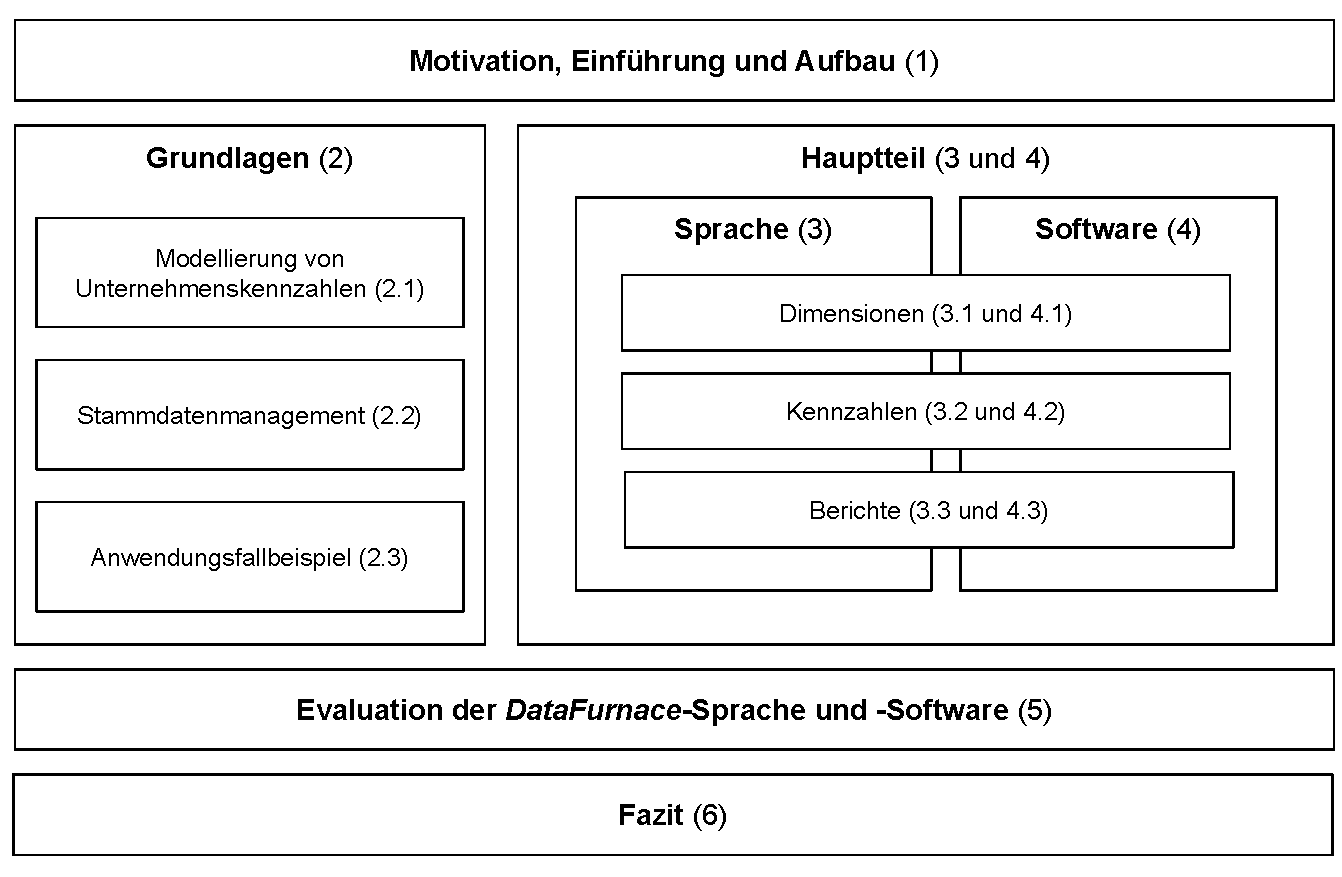
\includegraphics[scale=0.60]{content/figures/thesis-structure}
    \caption{Aufbau der Arbeit}\label{fig:thesis-structure}
  \end{figure}

  Der Hauptteil der Arbeit ist in zwei Abschnitte unterteilt, die Spezifikation
  der \textit{DataFurnace}-Sprache in Kapitel drei und die Implementierung der
  \textit{DataFurnace}-Software in Kapitel vier. Zunächst werden in Kapitel
  drei Anforderungen und Annahmen gesammelt, auf Basis dessen die Sprache
  entwickelt werden soll. Darauffolgend wird die Sprache anhand ihrer drei
  Grundpfeiler spezifiziert und erläutert mit jeweiliger Übertragung auf das
  Anwendungsfallbeispiel aus \cref{sec:anwendungsfallbeispiel}.  Der Aufbau des
  Kapitels vier ist stark an den des vorhergegangenen Kapitels drei zur
  \textit{DataFurnace}-Sprache angelehnt. Zunächst wird auf Anforderungen und
  Annahmen eingegangen, welche einen Rahmen für die Implementierung der
  \textit{DataFurnace}-Software geben sollen. Daraufhin wird die Software
  anhand ihrer drei Ansichten vorgestellt, welche jeweils auf die drei
  Grundpfeiler der Sprache zurück zu führen sind. Des Weiteren wird die
  Software im Zusammenhang des Anwendungsbeispiels exemplarisch eingesetzt.
  Zuletzt wird im Kapitel die Architektur der Software sowie einzelne
  technische Aspekte für die Erfüllung der Anforderungen thematisiert.

  Kapitel vier und Kapitel fünf schließen die Arbeit mit einer Evaluation und
  einem Fazit ab. Ersteres beurteilt die neue \textit{DataFurnace}-Sprache und
  -Software mit Hilfe von Nutzerbefragungen \todo{Wort ersetzen}, letzteres
  fasst die gewonnen Erkentnisse der Arbeit zusammen.  Der gesamte Aufbau der
  Arbeit wird erneut durch Abbildung~\ref{fig:thesis-structure} visualisiert.\todo{Grafik zum Aufbau der
  Arbeit}



  % ################################################################################
  \chapter{Grundlagen}\label{ch:grundlagen}
  % ################################################################################
  
  \todo[inline]{Grundlagen ca.\ 10 Seiten}
  \todo[inline]{Soll hier noch eine Einleitung zu dem Grundlagenkapitel hin?}

  \section{Modellierung}

  Für den konzeptionellen Umgang mit Unternehmensdaten existieren verschiedene
  Modelltypen, welche das Datenschema abstrahiert darstellen.  Die Modellierung
  der Daten ist essentiell für die Analyse:
  \textsc{\citeauthor{phipps2002automating}} zählen diese zu den fünf
  Hauptschritten der Datenanalyse im Data-Warehouse-Kontext~\cite[][S.
  1]{phipps2002automating}. Es wird nun die multidimensionale Modellierung
  beleuchtet und im Kontext der Unternehmensdatenanalyse mit der
  Entity-Relationship-Modellierung verglichen. Des Weiteren wird eine
  Erweiterung der multidimensionalen Modellierung--\textit{H2 for
  Reporting}--vorgestellt.


  \subsection{Multidimensionale
  Modellierung}\label{subsec:multidimensionale-modellierung} 

  Es gibt verschiedene Ausprägungen der multidimensionalen Modellierung.
  Zunächst wird auf allgemeine Eigenschaften der Modellierungsgruppe
  eingegangen. Im Mittelpunkt der multidimensionalen Modellierung stehen die
  betriebswirtschaftlichen Fakten~\cite[][S.  2]{phipps2002automating}. Ein
  Fakt kann eine Transaktion, ein Objekt oder ein Ereignis sein~\cite[][S.
  42]{ballard1998data}. \textsc{\citeauthor{Kemper2010}} nennt als Beispiele:
  \glqq{}Umsatzerlöse, Umsatzmengen, Einzelkosten oder den
  Personalbedarf\grqq{}~(\citeyear{Kemper2010}, S. 66). 

  Um verschiedene Sichten auf diese Fakten zu erlangen, gruppiert man diese in
  Dimensionen \bzw{} weist ihnen Dimensionsausprägungen zu~\cite[][S.
  66]{Kemper2010}. Dies ermöglicht es, in der späteren Analyse nach
  verschiedenen Dimensionen zu filtern und zu vergleichen. Dimensionen werden
  hierarchisch strukturiert. Mit Hilfe der daraus entstehenden Hierarchiestufen
  kann die Sicht auf die Daten in ihrem Detailgrad angepasst werden~\cite[][S.
  66]{Kemper2010}. Wege innerhalb der Dimension verlaufen nicht nur als
  einzelner Pfad linear, sondern auch als Struktur. Ein Beispiel ist die
  Dimension \textit{Zeit}.  Diese kann zum einen durch die
  Hierarchiestufenreihe \textit{Jahr, Monat, Tag} als auch durch \textit{Jahr,
  Woche, Tag} strukturiert werden (Siehe
  Abbildung~\ref{hierarchie-level-struktur}).\todo{Noch ein wenig holprig,
  bzw.\ ist das überhaupt relevant?}

  \begin{figure}
    \resizebox{100pt}{!}{% Graphic for TeX using PGF
% Title: /home/indenml/coding/bachelor_thesis/content/figures/hierarchie-level-struktur.dia
% Creator: Dia v0.97.3
% CreationDate: Thu Aug 11 18:24:55 2016
% For: indenml
% \usepackage{tikz}
% The following commands are not supported in PSTricks at present
% We define them conditionally, so when they are implemented,
% this pgf file will use them.
\ifx\du\undefined
  \newlength{\du}
\fi
\setlength{\du}{15\unitlength}
\begin{tikzpicture}
\pgftransformxscale{1.000000}
\pgftransformyscale{-1.000000}
\definecolor{dialinecolor}{rgb}{0.000000, 0.000000, 0.000000}
\pgfsetstrokecolor{dialinecolor}
\definecolor{dialinecolor}{rgb}{1.000000, 1.000000, 1.000000}
\pgfsetfillcolor{dialinecolor}
\definecolor{dialinecolor}{rgb}{1.000000, 1.000000, 1.000000}
\pgfsetfillcolor{dialinecolor}
\fill (5.050000\du,10.050000\du)--(5.050000\du,11.850000\du)--(7.990000\du,11.850000\du)--(7.990000\du,10.050000\du)--cycle;
\pgfsetlinewidth{0.100000\du}
\pgfsetdash{}{0pt}
\pgfsetmiterjoin
\definecolor{dialinecolor}{rgb}{0.000000, 0.000000, 0.000000}
\pgfsetstrokecolor{dialinecolor}
\draw (5.050000\du,10.050000\du)--(5.050000\du,11.850000\du)--(7.990000\du,11.850000\du)--(7.990000\du,10.050000\du)--cycle;
% setfont left to latex
\definecolor{dialinecolor}{rgb}{0.000000, 0.000000, 0.000000}
\pgfsetstrokecolor{dialinecolor}
\node at (6.520000\du,11.150000\du){Jahr};
\definecolor{dialinecolor}{rgb}{1.000000, 1.000000, 1.000000}
\pgfsetfillcolor{dialinecolor}
\fill (1.700000\du,13.050000\du)--(1.700000\du,14.850000\du)--(5.025000\du,14.850000\du)--(5.025000\du,13.050000\du)--cycle;
\pgfsetlinewidth{0.100000\du}
\pgfsetdash{}{0pt}
\pgfsetmiterjoin
\definecolor{dialinecolor}{rgb}{0.000000, 0.000000, 0.000000}
\pgfsetstrokecolor{dialinecolor}
\draw (1.700000\du,13.050000\du)--(1.700000\du,14.850000\du)--(5.025000\du,14.850000\du)--(5.025000\du,13.050000\du)--cycle;
% setfont left to latex
\definecolor{dialinecolor}{rgb}{0.000000, 0.000000, 0.000000}
\pgfsetstrokecolor{dialinecolor}
\node at (3.362500\du,14.150000\du){Monat};
\definecolor{dialinecolor}{rgb}{1.000000, 1.000000, 1.000000}
\pgfsetfillcolor{dialinecolor}
\fill (5.150000\du,16.550000\du)--(5.150000\du,18.350000\du)--(7.705000\du,18.350000\du)--(7.705000\du,16.550000\du)--cycle;
\pgfsetlinewidth{0.100000\du}
\pgfsetdash{}{0pt}
\pgfsetmiterjoin
\definecolor{dialinecolor}{rgb}{0.000000, 0.000000, 0.000000}
\pgfsetstrokecolor{dialinecolor}
\draw (5.150000\du,16.550000\du)--(5.150000\du,18.350000\du)--(7.705000\du,18.350000\du)--(7.705000\du,16.550000\du)--cycle;
% setfont left to latex
\definecolor{dialinecolor}{rgb}{0.000000, 0.000000, 0.000000}
\pgfsetstrokecolor{dialinecolor}
\node at (6.427500\du,17.650000\du){Tag};
\definecolor{dialinecolor}{rgb}{1.000000, 1.000000, 1.000000}
\pgfsetfillcolor{dialinecolor}
\fill (8.100000\du,13.050000\du)--(8.100000\du,14.850000\du)--(11.425000\du,14.850000\du)--(11.425000\du,13.050000\du)--cycle;
\pgfsetlinewidth{0.100000\du}
\pgfsetdash{}{0pt}
\pgfsetmiterjoin
\definecolor{dialinecolor}{rgb}{0.000000, 0.000000, 0.000000}
\pgfsetstrokecolor{dialinecolor}
\draw (8.100000\du,13.050000\du)--(8.100000\du,14.850000\du)--(11.425000\du,14.850000\du)--(11.425000\du,13.050000\du)--cycle;
% setfont left to latex
\definecolor{dialinecolor}{rgb}{0.000000, 0.000000, 0.000000}
\pgfsetstrokecolor{dialinecolor}
\node at (9.762500\du,14.150000\du){Woche};
\pgfsetlinewidth{0.100000\du}
\pgfsetdash{}{0pt}
\pgfsetdash{}{0pt}
\pgfsetmiterjoin
\pgfsetbuttcap
{
\definecolor{dialinecolor}{rgb}{0.000000, 0.000000, 0.000000}
\pgfsetfillcolor{dialinecolor}
% was here!!!
\pgfsetarrowsend{stealth}
{\pgfsetcornersarced{\pgfpoint{0.000000\du}{0.000000\du}}\definecolor{dialinecolor}{rgb}{0.000000, 0.000000, 0.000000}
\pgfsetstrokecolor{dialinecolor}
\draw (6.520000\du,11.850000\du)--(6.520000\du,12.125000\du)--(9.762500\du,12.125000\du)--(9.762500\du,13.050000\du);
}}
\pgfsetlinewidth{0.100000\du}
\pgfsetdash{}{0pt}
\pgfsetdash{}{0pt}
\pgfsetmiterjoin
\pgfsetbuttcap
{
\definecolor{dialinecolor}{rgb}{0.000000, 0.000000, 0.000000}
\pgfsetfillcolor{dialinecolor}
% was here!!!
\pgfsetarrowsend{stealth}
{\pgfsetcornersarced{\pgfpoint{0.000000\du}{0.000000\du}}\definecolor{dialinecolor}{rgb}{0.000000, 0.000000, 0.000000}
\pgfsetstrokecolor{dialinecolor}
\draw (6.520000\du,11.850000\du)--(6.520000\du,12.125000\du)--(3.362500\du,12.125000\du)--(3.362500\du,13.050000\du);
}}
\pgfsetlinewidth{0.100000\du}
\pgfsetdash{}{0pt}
\pgfsetdash{}{0pt}
\pgfsetmiterjoin
\pgfsetbuttcap
{
\definecolor{dialinecolor}{rgb}{0.000000, 0.000000, 0.000000}
\pgfsetfillcolor{dialinecolor}
% was here!!!
\pgfsetarrowsend{stealth}
{\pgfsetcornersarced{\pgfpoint{0.000000\du}{0.000000\du}}\definecolor{dialinecolor}{rgb}{0.000000, 0.000000, 0.000000}
\pgfsetstrokecolor{dialinecolor}
\draw (9.762500\du,14.850000\du)--(9.762500\du,15.525000\du)--(6.427500\du,15.525000\du)--(6.427500\du,16.550000\du);
}}
\pgfsetlinewidth{0.100000\du}
\pgfsetdash{}{0pt}
\pgfsetdash{}{0pt}
\pgfsetmiterjoin
\pgfsetbuttcap
{
\definecolor{dialinecolor}{rgb}{0.000000, 0.000000, 0.000000}
\pgfsetfillcolor{dialinecolor}
% was here!!!
\pgfsetarrowsend{stealth}
{\pgfsetcornersarced{\pgfpoint{0.000000\du}{0.000000\du}}\definecolor{dialinecolor}{rgb}{0.000000, 0.000000, 0.000000}
\pgfsetstrokecolor{dialinecolor}
\draw (3.362500\du,14.850000\du)--(3.362500\du,15.525000\du)--(6.427500\du,15.525000\du)--(6.427500\du,16.550000\du);
}}
\end{tikzpicture}
}
    \caption{Dimensionslevelstruktur der Beispieldimension Zeit}\label{hierarchie-level-struktur}
  \end{figure}

	Die multidimensionale Modellierung unterteilt sich nun in verschiedene
	Ausprägungen.  Die bekannteste Ausprägung ist das Star-Modell~\cite[][S.
	2]{phipps2002automating}\todo{Wird auf das Star-Modell im Hauptteil
	verwiesen?}. Der Name ist zurückzuführen auf den Aufbau eines
	entsprechenden Modells (Siehe Abbildung~\ref{fig:star-schema}), welches die
	Form eines Sterns hat~\cite[][S.  44]{Kimball2013}. In der Mitte des Sterns
	befindet sich die Faktentabelle~\cite[][S. 67]{Kemper2010}. Diese verweist
	mit Hilfe von Fremdschlüsseln auf Dimensionstabellen, welche jeweils eine
	komplette Dimension abbilden und somit im Gegenzug auf die dritte Normalform
	verzichten~\cite[][S. 67 f.]{Kemper2010}. Die bestehende Datenredundanz
	(Siehe Abbildung~\ref{table:dimension-table}) durch Mangel an Normalisierung
	in den Dimensionstabellen, resultiert laut \textsc{\citeauthor{Kimball2013}}
	durch ihre geringe Größe nicht in einer schlechteren Leistung des
	Datenbanksystems, sondern im Gegenzug in einer besseren Verständlichkeit der
	Struktur~\cite[][S. 15]{Kimball2013}. Weitere Details zur
	Datenbanknormalisierung können in den Publikationen des
	Begründers \todo{Erfinder oder Begründer das richtige Wort?}
	\textsc{\citeauthor{codd1970relational}} gefunden
	werden~\citeyearpar{codd1970relational,codd1972further}.

  \begin{figure}
    \resizebox{0.5\linewidth}{!}{% Graphic for TeX using PGF
% Title: /home/indenml/code/bachelor_thesis/content/figures/star-schema.dia
% Creator: Dia v0.97.3
% CreationDate: Thu Sep 29 00:10:53 2016
% For: indenml
% \usepackage{tikz}
% The following commands are not supported in PSTricks at present
% We define them conditionally, so when they are implemented,
% this pgf file will use them.
\ifx\du\undefined{}
  \newlength{\du}
\fi
\setlength{\du}{15\unitlength}
\begin{tikzpicture}
\pgftransformxscale{1.000000}
\pgftransformyscale{-1.000000}
\definecolor{dialinecolor}{rgb}{0.000000, 0.000000, 0.000000}
\pgfsetstrokecolor{dialinecolor}
\definecolor{dialinecolor}{rgb}{1.000000, 1.000000, 1.000000}
\pgfsetfillcolor{dialinecolor}
\pgfsetlinewidth{0.100000\du}
\pgfsetdash{}{0pt}
\definecolor{dialinecolor}{rgb}{1.000000, 1.000000, 1.000000}
\pgfsetfillcolor{dialinecolor}
\fill (12.100000\du,6.600000\du)--(12.100000\du,8.000000\du)--(19.005000\du,8.000000\du)--(19.005000\du,6.600000\du)--cycle;
\definecolor{dialinecolor}{rgb}{0.000000, 0.000000, 0.000000}
\pgfsetstrokecolor{dialinecolor}
\draw (12.100000\du,6.600000\du)--(12.100000\du,8.000000\du)--(19.005000\du,8.000000\du)--(19.005000\du,6.600000\du)--cycle;
% setfont left to latex
\definecolor{dialinecolor}{rgb}{0.000000, 0.000000, 0.000000}
\pgfsetstrokecolor{dialinecolor}
\node at (15.552500\du,7.550000\du){Umsatzmenge};
\definecolor{dialinecolor}{rgb}{1.000000, 1.000000, 1.000000}
\pgfsetfillcolor{dialinecolor}
\fill (12.100000\du,8.000000\du)--(12.100000\du,13.800000\du)--(19.005000\du,13.800000\du)--(19.005000\du,8.000000\du)--cycle;
\definecolor{dialinecolor}{rgb}{0.000000, 0.000000, 0.000000}
\pgfsetstrokecolor{dialinecolor}
\draw (12.100000\du,8.000000\du)--(12.100000\du,13.800000\du)--(19.005000\du,13.800000\du)--(19.005000\du,8.000000\du)--cycle;
% setfont left to latex
\definecolor{dialinecolor}{rgb}{0.000000, 0.000000, 0.000000}
\pgfsetstrokecolor{dialinecolor}
\node[anchor=west] at (12.250000\du,8.700000\du){Zeit Id};
% setfont left to latex
\definecolor{dialinecolor}{rgb}{0.000000, 0.000000, 0.000000}
\pgfsetstrokecolor{dialinecolor}
\node[anchor=west] at (12.250000\du,9.500000\du){Ort Id};
% setfont left to latex
\definecolor{dialinecolor}{rgb}{0.000000, 0.000000, 0.000000}
\pgfsetstrokecolor{dialinecolor}
\node[anchor=west] at (12.250000\du,10.300000\du){Absatzkanal Id};
% setfont left to latex
\definecolor{dialinecolor}{rgb}{0.000000, 0.000000, 0.000000}
\pgfsetstrokecolor{dialinecolor}
\node[anchor=west] at (12.250000\du,11.100000\du){Personal Id};
% setfont left to latex
\definecolor{dialinecolor}{rgb}{0.000000, 0.000000, 0.000000}
\pgfsetstrokecolor{dialinecolor}
\node[anchor=west] at (12.250000\du,11.900000\du){Kunde Id};
% setfont left to latex
\definecolor{dialinecolor}{rgb}{0.000000, 0.000000, 0.000000}
\pgfsetstrokecolor{dialinecolor}
\node[anchor=west] at (12.250000\du,12.700000\du){Produkt Id};
% setfont left to latex
\definecolor{dialinecolor}{rgb}{0.000000, 0.000000, 0.000000}
\pgfsetstrokecolor{dialinecolor}
\node[anchor=west] at (12.250000\du,13.500000\du){};
\pgfsetlinewidth{0.100000\du}
\pgfsetdash{}{0pt}
\definecolor{dialinecolor}{rgb}{1.000000, 1.000000, 1.000000}
\pgfsetfillcolor{dialinecolor}
\fill (4.100000\du,1.200000\du)--(4.100000\du,2.600000\du)--(7.680000\du,2.600000\du)--(7.680000\du,1.200000\du)--cycle;
\definecolor{dialinecolor}{rgb}{0.000000, 0.000000, 0.000000}
\pgfsetstrokecolor{dialinecolor}
\draw (4.100000\du,1.200000\du)--(4.100000\du,2.600000\du)--(7.680000\du,2.600000\du)--(7.680000\du,1.200000\du)--cycle;
% setfont left to latex
\definecolor{dialinecolor}{rgb}{0.000000, 0.000000, 0.000000}
\pgfsetstrokecolor{dialinecolor}
\node at (5.890000\du,2.150000\du){Zeit};
\definecolor{dialinecolor}{rgb}{1.000000, 1.000000, 1.000000}
\pgfsetfillcolor{dialinecolor}
\fill (4.100000\du,2.600000\du)--(4.100000\du,7.600000\du)--(7.680000\du,7.600000\du)--(7.680000\du,2.600000\du)--cycle;
\definecolor{dialinecolor}{rgb}{0.000000, 0.000000, 0.000000}
\pgfsetstrokecolor{dialinecolor}
\draw (4.100000\du,2.600000\du)--(4.100000\du,7.600000\du)--(7.680000\du,7.600000\du)--(7.680000\du,2.600000\du)--cycle;
% setfont left to latex
\definecolor{dialinecolor}{rgb}{0.000000, 0.000000, 0.000000}
\pgfsetstrokecolor{dialinecolor}
\node[anchor=west] at (4.250000\du,3.300000\du){Zeit Id};
% setfont left to latex
\definecolor{dialinecolor}{rgb}{0.000000, 0.000000, 0.000000}
\pgfsetstrokecolor{dialinecolor}
\node[anchor=west] at (4.250000\du,4.100000\du){Tag};
% setfont left to latex
\definecolor{dialinecolor}{rgb}{0.000000, 0.000000, 0.000000}
\pgfsetstrokecolor{dialinecolor}
\node[anchor=west] at (4.250000\du,4.900000\du){Woche};
% setfont left to latex
\definecolor{dialinecolor}{rgb}{0.000000, 0.000000, 0.000000}
\pgfsetstrokecolor{dialinecolor}
\node[anchor=west] at (4.250000\du,5.700000\du){Monat};
% setfont left to latex
\definecolor{dialinecolor}{rgb}{0.000000, 0.000000, 0.000000}
\pgfsetstrokecolor{dialinecolor}
\node[anchor=west] at (4.250000\du,6.500000\du){Jahr};
% setfont left to latex
\definecolor{dialinecolor}{rgb}{0.000000, 0.000000, 0.000000}
\pgfsetstrokecolor{dialinecolor}
\node[anchor=west] at (4.250000\du,7.300000\du){};
\pgfsetlinewidth{0.100000\du}
\pgfsetdash{}{0pt}
\definecolor{dialinecolor}{rgb}{1.000000, 1.000000, 1.000000}
\pgfsetfillcolor{dialinecolor}
\fill (5.800000\du,12.800000\du)--(5.800000\du,14.200000\du)--(8.995000\du,14.200000\du)--(8.995000\du,12.800000\du)--cycle;
\definecolor{dialinecolor}{rgb}{0.000000, 0.000000, 0.000000}
\pgfsetstrokecolor{dialinecolor}
\draw (5.800000\du,12.800000\du)--(5.800000\du,14.200000\du)--(8.995000\du,14.200000\du)--(8.995000\du,12.800000\du)--cycle;
% setfont left to latex
\definecolor{dialinecolor}{rgb}{0.000000, 0.000000, 0.000000}
\pgfsetstrokecolor{dialinecolor}
\node at (7.397500\du,13.750000\du){Ort};
\definecolor{dialinecolor}{rgb}{1.000000, 1.000000, 1.000000}
\pgfsetfillcolor{dialinecolor}
\fill (5.800000\du,14.200000\du)--(5.800000\du,18.400000\du)--(8.995000\du,18.400000\du)--(8.995000\du,14.200000\du)--cycle;
\definecolor{dialinecolor}{rgb}{0.000000, 0.000000, 0.000000}
\pgfsetstrokecolor{dialinecolor}
\draw (5.800000\du,14.200000\du)--(5.800000\du,18.400000\du)--(8.995000\du,18.400000\du)--(8.995000\du,14.200000\du)--cycle;
% setfont left to latex
\definecolor{dialinecolor}{rgb}{0.000000, 0.000000, 0.000000}
\pgfsetstrokecolor{dialinecolor}
\node[anchor=west] at (5.950000\du,14.900000\du){Ort Id};
% setfont left to latex
\definecolor{dialinecolor}{rgb}{0.000000, 0.000000, 0.000000}
\pgfsetstrokecolor{dialinecolor}
\node[anchor=west] at (5.950000\du,15.700000\du){Straße};
% setfont left to latex
\definecolor{dialinecolor}{rgb}{0.000000, 0.000000, 0.000000}
\pgfsetstrokecolor{dialinecolor}
\node[anchor=west] at (5.950000\du,16.500000\du){Ort};
% setfont left to latex
\definecolor{dialinecolor}{rgb}{0.000000, 0.000000, 0.000000}
\pgfsetstrokecolor{dialinecolor}
\node[anchor=west] at (5.950000\du,17.300000\du){Land};
% setfont left to latex
\definecolor{dialinecolor}{rgb}{0.000000, 0.000000, 0.000000}
\pgfsetstrokecolor{dialinecolor}
\node[anchor=west] at (5.950000\du,18.100000\du){};
\pgfsetlinewidth{0.100000\du}
\pgfsetdash{}{0pt}
\definecolor{dialinecolor}{rgb}{1.000000, 1.000000, 1.000000}
\pgfsetfillcolor{dialinecolor}
\fill (22.150000\du,2.650000\du)--(22.150000\du,4.050000\du)--(28.040000\du,4.050000\du)--(28.040000\du,2.650000\du)--cycle;
\definecolor{dialinecolor}{rgb}{0.000000, 0.000000, 0.000000}
\pgfsetstrokecolor{dialinecolor}
\draw (22.150000\du,2.650000\du)--(22.150000\du,4.050000\du)--(28.040000\du,4.050000\du)--(28.040000\du,2.650000\du)--cycle;
% setfont left to latex
\definecolor{dialinecolor}{rgb}{0.000000, 0.000000, 0.000000}
\pgfsetstrokecolor{dialinecolor}
\node at (25.095000\du,3.600000\du){Kunde};
\definecolor{dialinecolor}{rgb}{1.000000, 1.000000, 1.000000}
\pgfsetfillcolor{dialinecolor}
\fill (22.150000\du,4.050000\du)--(22.150000\du,7.450000\du)--(28.040000\du,7.450000\du)--(28.040000\du,4.050000\du)--cycle;
\definecolor{dialinecolor}{rgb}{0.000000, 0.000000, 0.000000}
\pgfsetstrokecolor{dialinecolor}
\draw (22.150000\du,4.050000\du)--(22.150000\du,7.450000\du)--(28.040000\du,7.450000\du)--(28.040000\du,4.050000\du)--cycle;
% setfont left to latex
\definecolor{dialinecolor}{rgb}{0.000000, 0.000000, 0.000000}
\pgfsetstrokecolor{dialinecolor}
\node[anchor=west] at (22.300000\du,4.750000\du){Kunden Id};
% setfont left to latex
\definecolor{dialinecolor}{rgb}{0.000000, 0.000000, 0.000000}
\pgfsetstrokecolor{dialinecolor}
\node[anchor=west] at (22.300000\du,5.550000\du){Kundengruppe};
% setfont left to latex
\definecolor{dialinecolor}{rgb}{0.000000, 0.000000, 0.000000}
\pgfsetstrokecolor{dialinecolor}
\node[anchor=west] at (22.300000\du,6.350000\du){Kundensegment};
% setfont left to latex
\definecolor{dialinecolor}{rgb}{0.000000, 0.000000, 0.000000}
\pgfsetstrokecolor{dialinecolor}
\node[anchor=west] at (22.300000\du,7.150000\du){};
\pgfsetlinewidth{0.100000\du}
\pgfsetdash{}{0pt}
\definecolor{dialinecolor}{rgb}{1.000000, 1.000000, 1.000000}
\pgfsetfillcolor{dialinecolor}
\fill (21.350000\du,13.550000\du)--(21.350000\du,14.950000\du)--(27.625000\du,14.950000\du)--(27.625000\du,13.550000\du)--cycle;
\definecolor{dialinecolor}{rgb}{0.000000, 0.000000, 0.000000}
\pgfsetstrokecolor{dialinecolor}
\draw (21.350000\du,13.550000\du)--(21.350000\du,14.950000\du)--(27.625000\du,14.950000\du)--(27.625000\du,13.550000\du)--cycle;
% setfont left to latex
\definecolor{dialinecolor}{rgb}{0.000000, 0.000000, 0.000000}
\pgfsetstrokecolor{dialinecolor}
\node at (24.487500\du,14.500000\du){Personal};
\definecolor{dialinecolor}{rgb}{1.000000, 1.000000, 1.000000}
\pgfsetfillcolor{dialinecolor}
\fill (21.350000\du,14.950000\du)--(21.350000\du,18.350000\du)--(27.625000\du,18.350000\du)--(27.625000\du,14.950000\du)--cycle;
\definecolor{dialinecolor}{rgb}{0.000000, 0.000000, 0.000000}
\pgfsetstrokecolor{dialinecolor}
\draw (21.350000\du,14.950000\du)--(21.350000\du,18.350000\du)--(27.625000\du,18.350000\du)--(27.625000\du,14.950000\du)--cycle;
% setfont left to latex
\definecolor{dialinecolor}{rgb}{0.000000, 0.000000, 0.000000}
\pgfsetstrokecolor{dialinecolor}
\node[anchor=west] at (21.500000\du,15.650000\du){Personal Id};
% setfont left to latex
\definecolor{dialinecolor}{rgb}{0.000000, 0.000000, 0.000000}
\pgfsetstrokecolor{dialinecolor}
\node[anchor=west] at (21.500000\du,16.450000\du){Unterabteilung};
% setfont left to latex
\definecolor{dialinecolor}{rgb}{0.000000, 0.000000, 0.000000}
\pgfsetstrokecolor{dialinecolor}
\node[anchor=west] at (21.500000\du,17.250000\du){Abteilung};
% setfont left to latex
\definecolor{dialinecolor}{rgb}{0.000000, 0.000000, 0.000000}
\pgfsetstrokecolor{dialinecolor}
\node[anchor=west] at (21.500000\du,18.050000\du){};
\pgfsetlinewidth{0.100000\du}
\pgfsetdash{}{0pt}
\definecolor{dialinecolor}{rgb}{1.000000, 1.000000, 1.000000}
\pgfsetfillcolor{dialinecolor}
\fill (1.650000\du,8.250000\du)--(1.650000\du,9.650000\du)--(7.925000\du,9.650000\du)--(7.925000\du,8.250000\du)--cycle;
\definecolor{dialinecolor}{rgb}{0.000000, 0.000000, 0.000000}
\pgfsetstrokecolor{dialinecolor}
\draw (1.650000\du,8.250000\du)--(1.650000\du,9.650000\du)--(7.925000\du,9.650000\du)--(7.925000\du,8.250000\du)--cycle;
% setfont left to latex
\definecolor{dialinecolor}{rgb}{0.000000, 0.000000, 0.000000}
\pgfsetstrokecolor{dialinecolor}
\node at (4.787500\du,9.200000\du){Absatzkanal};
\definecolor{dialinecolor}{rgb}{1.000000, 1.000000, 1.000000}
\pgfsetfillcolor{dialinecolor}
\fill (1.650000\du,9.650000\du)--(1.650000\du,12.250000\du)--(7.925000\du,12.250000\du)--(7.925000\du,9.650000\du)--cycle;
\definecolor{dialinecolor}{rgb}{0.000000, 0.000000, 0.000000}
\pgfsetstrokecolor{dialinecolor}
\draw (1.650000\du,9.650000\du)--(1.650000\du,12.250000\du)--(7.925000\du,12.250000\du)--(7.925000\du,9.650000\du)--cycle;
% setfont left to latex
\definecolor{dialinecolor}{rgb}{0.000000, 0.000000, 0.000000}
\pgfsetstrokecolor{dialinecolor}
\node[anchor=west] at (1.800000\du,10.350000\du){Absatzkanal Id};
% setfont left to latex
\definecolor{dialinecolor}{rgb}{0.000000, 0.000000, 0.000000}
\pgfsetstrokecolor{dialinecolor}
\node[anchor=west] at (1.800000\du,11.150000\du){Absatzgruppe};
% setfont left to latex
\definecolor{dialinecolor}{rgb}{0.000000, 0.000000, 0.000000}
\pgfsetstrokecolor{dialinecolor}
\node[anchor=west] at (1.800000\du,11.950000\du){};
\pgfsetlinewidth{0.100000\du}
\pgfsetdash{}{0pt}
\definecolor{dialinecolor}{rgb}{1.000000, 1.000000, 1.000000}
\pgfsetfillcolor{dialinecolor}
\fill (22.750000\du,8.250000\du)--(22.750000\du,9.650000\du)--(29.795000\du,9.650000\du)--(29.795000\du,8.250000\du)--cycle;
\definecolor{dialinecolor}{rgb}{0.000000, 0.000000, 0.000000}
\pgfsetstrokecolor{dialinecolor}
\draw (22.750000\du,8.250000\du)--(22.750000\du,9.650000\du)--(29.795000\du,9.650000\du)--(29.795000\du,8.250000\du)--cycle;
% setfont left to latex
\definecolor{dialinecolor}{rgb}{0.000000, 0.000000, 0.000000}
\pgfsetstrokecolor{dialinecolor}
\node at (26.272500\du,9.200000\du){Produkt};
\definecolor{dialinecolor}{rgb}{1.000000, 1.000000, 1.000000}
\pgfsetfillcolor{dialinecolor}
\fill (22.750000\du,9.650000\du)--(22.750000\du,13.050000\du)--(29.795000\du,13.050000\du)--(29.795000\du,9.650000\du)--cycle;
\definecolor{dialinecolor}{rgb}{0.000000, 0.000000, 0.000000}
\pgfsetstrokecolor{dialinecolor}
\draw (22.750000\du,9.650000\du)--(22.750000\du,13.050000\du)--(29.795000\du,13.050000\du)--(29.795000\du,9.650000\du)--cycle;
% setfont left to latex
\definecolor{dialinecolor}{rgb}{0.000000, 0.000000, 0.000000}
\pgfsetstrokecolor{dialinecolor}
\node[anchor=west] at (22.900000\du,10.350000\du){Produkt Id};
% setfont left to latex
\definecolor{dialinecolor}{rgb}{0.000000, 0.000000, 0.000000}
\pgfsetstrokecolor{dialinecolor}
\node[anchor=west] at (22.900000\du,11.150000\du){Produktkategorie};
% setfont left to latex
\definecolor{dialinecolor}{rgb}{0.000000, 0.000000, 0.000000}
\pgfsetstrokecolor{dialinecolor}
\node[anchor=west] at (22.900000\du,11.950000\du){Produktlinie};
% setfont left to latex
\definecolor{dialinecolor}{rgb}{0.000000, 0.000000, 0.000000}
\pgfsetstrokecolor{dialinecolor}
\node[anchor=west] at (22.900000\du,12.750000\du){};
\pgfsetlinewidth{0.100000\du}
\pgfsetdash{}{0pt}
\pgfsetdash{}{0pt}
\pgfsetbuttcap
{\definecolor{dialinecolor}{rgb}{0.000000, 0.000000, 0.000000}
\pgfsetfillcolor{dialinecolor}
% was here!!!
\definecolor{dialinecolor}{rgb}{0.000000, 0.000000, 0.000000}
\pgfsetstrokecolor{dialinecolor}
\draw (19.005000\du,10.100000\du)--(22.750000\du,10.150000\du);
}
\pgfsetlinewidth{0.100000\du}
\pgfsetdash{}{0pt}
\pgfsetdash{}{0pt}
\pgfsetbuttcap
{\definecolor{dialinecolor}{rgb}{0.000000, 0.000000, 0.000000}
\pgfsetfillcolor{dialinecolor}
% was here!!!
\definecolor{dialinecolor}{rgb}{0.000000, 0.000000, 0.000000}
\pgfsetstrokecolor{dialinecolor}
\draw (8.995000\du,14.700000\du)--(12.100000\du,13.800000\du);
}
\pgfsetlinewidth{0.100000\du}
\pgfsetdash{}{0pt}
\pgfsetdash{}{0pt}
\pgfsetbuttcap
{\definecolor{dialinecolor}{rgb}{0.000000, 0.000000, 0.000000}
\pgfsetfillcolor{dialinecolor}
% was here!!!
\definecolor{dialinecolor}{rgb}{0.000000, 0.000000, 0.000000}
\pgfsetstrokecolor{dialinecolor}
\draw (7.925000\du,10.150000\du)--(12.100000\du,10.100000\du);
}
\pgfsetlinewidth{0.100000\du}
\pgfsetdash{}{0pt}
\pgfsetdash{}{0pt}
\pgfsetbuttcap
{\definecolor{dialinecolor}{rgb}{0.000000, 0.000000, 0.000000}
\pgfsetfillcolor{dialinecolor}
% was here!!!
\definecolor{dialinecolor}{rgb}{0.000000, 0.000000, 0.000000}
\pgfsetstrokecolor{dialinecolor}
\draw (19.005000\du,6.600000\du)--(22.150000\du,4.550000\du);
}
\pgfsetlinewidth{0.100000\du}
\pgfsetdash{}{0pt}
\pgfsetdash{}{0pt}
\pgfsetbuttcap
{\definecolor{dialinecolor}{rgb}{0.000000, 0.000000, 0.000000}
\pgfsetfillcolor{dialinecolor}
% was here!!!
\definecolor{dialinecolor}{rgb}{0.000000, 0.000000, 0.000000}
\pgfsetstrokecolor{dialinecolor}
\draw (21.350000\du,15.450000\du)--(19.005000\du,13.800000\du);
}
\pgfsetlinewidth{0.100000\du}
\pgfsetdash{}{0pt}
\pgfsetdash{}{0pt}
\pgfsetbuttcap
{\definecolor{dialinecolor}{rgb}{0.000000, 0.000000, 0.000000}
\pgfsetfillcolor{dialinecolor}
% was here!!!
\definecolor{dialinecolor}{rgb}{0.000000, 0.000000, 0.000000}
\pgfsetstrokecolor{dialinecolor}
\draw (7.680000\du,3.900000\du)--(12.100000\du,6.600000\du);
}
\end{tikzpicture}
}
    \caption[Star-Schema Beispielmodell]{Star-Schema Beispielmodell angelehnt an~\cite{Kemper2010} Abb. 2.30}\label{fig:star-schema}
  \end{figure}

  \begin{table}[]
    \footnotesize
    \begin{tabular}{c c c c}
      Ort Id & Straße & Ort & Land \\
      \toprule
      0 & Corrensstraße & Münster & Deutschland \\
      1 & Rudolf-Harbig-Weg & Münster & Deutschland \\
      2 & Hauptstraße & Bonn & Deutschland \\
    \end{tabular}
    \caption{Beispiel der Dimensionstabelle \textit{Ort} im Star-Schema}\label{table:dimension-table}
  \end{table}

  Eine weitere Ausprägung der multidimensionalen Modellierung ist das Snowflake-Modell.
  Analog zum Star-Modell gleicht die Form eines Snowflake-Modells einer
  Schneeflocke~\cite[][S. 70]{Kemper2010}. Star- und Snowflake-Modell
  unterscheiden sich in der Datenhaltung der Dimensionstabellen. Wie bereits im
  vorherigen Absatz beschrieben verfolgt das Star-Schema einen denormalisierten
  Ansatz, wohingegen die Dimensionstabellen des Snowflak-Modells normalisiert
  sind~\cite[][S. 70]{Kemper2010}. Abbildung~\ref{fig:snowflake-schema}
  visualisiert die strenge Normalisierung an der Dimension Ort.
  Abbildung~\ref{table:dimension-table-snow} zeigt konkrete Beispieldaten dieser
  Dimension in Form von Tabellen.  \textsc{\citeauthor{Kemper2010}} schlägt alternativ
  nicht den Ansatz der vollen Normalisierung im Snowflake-Modell vor, sondern eine
  geschwindigkeitsorientierte Teilnormalisierung~(\citeyear{Kemper2010}, S. 70).
  \textsc{\citeauthor{Kimball2013}} hingegen raten komplett vom Snowflake-Modell
  ab, da es ihrer Meinung nach sowohl die Verständlichkeit als auch gegebenenfalls die
  Geschwindigkeit negativ beeinträchtigt~(\citeyear{Kimball2013}, S. 50).

  \begin{figure}
    \resizebox{250pt}{!}{% Graphic for TeX using PGF
% Title: /home/indenml/coding/bachelor_thesis/content/figures/snowflake-schema.dia
% Creator: Dia v0.97.3
% CreationDate: Thu Aug 11 17:57:36 2016
% For: indenml
% \usepackage{tikz}
% The following commands are not supported in PSTricks at present
% We define them conditionally, so when they are implemented,
% this pgf file will use them.
\ifx\du\undefined{}
  \newlength{\du}
\fi
\setlength{\du}{15\unitlength}
\begin{tikzpicture}
\pgftransformxscale{1.000000}
\pgftransformyscale{-1.000000}
\definecolor{dialinecolor}{rgb}{0.000000, 0.000000, 0.000000}
\pgfsetstrokecolor{dialinecolor}
\definecolor{dialinecolor}{rgb}{1.000000, 1.000000, 1.000000}
\pgfsetfillcolor{dialinecolor}
\pgfsetlinewidth{0.100000\du}
\pgfsetdash{}{0pt}
\definecolor{dialinecolor}{rgb}{1.000000, 1.000000, 1.000000}
\pgfsetfillcolor{dialinecolor}
\fill (23.150000\du,13.700000\du)--(23.150000\du,15.100000\du)--(30.055000\du,15.100000\du)--(30.055000\du,13.700000\du)--cycle;
\definecolor{dialinecolor}{rgb}{0.000000, 0.000000, 0.000000}
\pgfsetstrokecolor{dialinecolor}
\draw (23.150000\du,13.700000\du)--(23.150000\du,15.100000\du)--(30.055000\du,15.100000\du)--(30.055000\du,13.700000\du)--cycle;
% setfont left to latex
\definecolor{dialinecolor}{rgb}{0.000000, 0.000000, 0.000000}
\pgfsetstrokecolor{dialinecolor}
\node at (26.602500\du,14.650000\du){Umsatzmenge};
\definecolor{dialinecolor}{rgb}{1.000000, 1.000000, 1.000000}
\pgfsetfillcolor{dialinecolor}
\fill (23.150000\du,15.100000\du)--(23.150000\du,20.900000\du)--(30.055000\du,20.900000\du)--(30.055000\du,15.100000\du)--cycle;
\definecolor{dialinecolor}{rgb}{0.000000, 0.000000, 0.000000}
\pgfsetstrokecolor{dialinecolor}
\draw (23.150000\du,15.100000\du)--(23.150000\du,20.900000\du)--(30.055000\du,20.900000\du)--(30.055000\du,15.100000\du)--cycle;
% setfont left to latex
\definecolor{dialinecolor}{rgb}{0.000000, 0.000000, 0.000000}
\pgfsetstrokecolor{dialinecolor}
\node[anchor=west] at (23.300000\du,15.800000\du){Zeit Id};
% setfont left to latex
\definecolor{dialinecolor}{rgb}{0.000000, 0.000000, 0.000000}
\pgfsetstrokecolor{dialinecolor}
\node[anchor=west] at (23.300000\du,16.600000\du){Straße Id};
% setfont left to latex
\definecolor{dialinecolor}{rgb}{0.000000, 0.000000, 0.000000}
\pgfsetstrokecolor{dialinecolor}
\node[anchor=west] at (23.300000\du,17.400000\du){Absatzkanal Id};
% setfont left to latex
\definecolor{dialinecolor}{rgb}{0.000000, 0.000000, 0.000000}
\pgfsetstrokecolor{dialinecolor}
\node[anchor=west] at (23.300000\du,18.200000\du){Personal Id};
% setfont left to latex
\definecolor{dialinecolor}{rgb}{0.000000, 0.000000, 0.000000}
\pgfsetstrokecolor{dialinecolor}
\node[anchor=west] at (23.300000\du,19.000000\du){Kunde Id};
% setfont left to latex
\definecolor{dialinecolor}{rgb}{0.000000, 0.000000, 0.000000}
\pgfsetstrokecolor{dialinecolor}
\node[anchor=west] at (23.300000\du,19.800000\du){Produkt Id};
% setfont left to latex
\definecolor{dialinecolor}{rgb}{0.000000, 0.000000, 0.000000}
\pgfsetstrokecolor{dialinecolor}
\node[anchor=west] at (23.300000\du,20.600000\du){};
\pgfsetlinewidth{0.100000\du}
\pgfsetdash{}{0pt}
\definecolor{dialinecolor}{rgb}{1.000000, 1.000000, 1.000000}
\pgfsetfillcolor{dialinecolor}
\fill (16.700000\du,15.297000\du)--(16.700000\du,16.697000\du)--(21.050000\du,16.697000\du)--(21.050000\du,15.297000\du)--cycle;
\definecolor{dialinecolor}{rgb}{0.000000, 0.000000, 0.000000}
\pgfsetstrokecolor{dialinecolor}
\draw (16.700000\du,15.297000\du)--(16.700000\du,16.697000\du)--(21.050000\du,16.697000\du)--(21.050000\du,15.297000\du)--cycle;
% setfont left to latex
\definecolor{dialinecolor}{rgb}{0.000000, 0.000000, 0.000000}
\pgfsetstrokecolor{dialinecolor}
\node at (18.875000\du,16.247000\du){Straße};
\definecolor{dialinecolor}{rgb}{1.000000, 1.000000, 1.000000}
\pgfsetfillcolor{dialinecolor}
\fill (16.700000\du,16.697000\du)--(16.700000\du,20.097000\du)--(21.050000\du,20.097000\du)--(21.050000\du,16.697000\du)--cycle;
\definecolor{dialinecolor}{rgb}{0.000000, 0.000000, 0.000000}
\pgfsetstrokecolor{dialinecolor}
\draw (16.700000\du,16.697000\du)--(16.700000\du,20.097000\du)--(21.050000\du,20.097000\du)--(21.050000\du,16.697000\du)--cycle;
% setfont left to latex
\definecolor{dialinecolor}{rgb}{0.000000, 0.000000, 0.000000}
\pgfsetstrokecolor{dialinecolor}
\node[anchor=west] at (16.850000\du,17.397000\du){Straße Id};
% setfont left to latex
\definecolor{dialinecolor}{rgb}{0.000000, 0.000000, 0.000000}
\pgfsetstrokecolor{dialinecolor}
\node[anchor=west] at (16.850000\du,18.197000\du){Name};
% setfont left to latex
\definecolor{dialinecolor}{rgb}{0.000000, 0.000000, 0.000000}
\pgfsetstrokecolor{dialinecolor}
\node[anchor=west] at (16.850000\du,18.997000\du){Ort Id};
% setfont left to latex
\definecolor{dialinecolor}{rgb}{0.000000, 0.000000, 0.000000}
\pgfsetstrokecolor{dialinecolor}
\node[anchor=west] at (16.850000\du,19.797000\du){};
\pgfsetlinewidth{0.100000\du}
\pgfsetdash{}{0pt}
\pgfsetdash{}{0pt}
\pgfsetbuttcap
{\definecolor{dialinecolor}{rgb}{0.000000, 0.000000, 0.000000}
\pgfsetfillcolor{dialinecolor}
% was here!!!
\definecolor{dialinecolor}{rgb}{0.000000, 0.000000, 0.000000}
\pgfsetstrokecolor{dialinecolor}
\draw (21.050000\du,17.197000\du)--(23.150000\du,17.200000\du);
}
\pgfsetlinewidth{0.100000\du}
\pgfsetdash{}{0pt}
\definecolor{dialinecolor}{rgb}{1.000000, 1.000000, 1.000000}
\pgfsetfillcolor{dialinecolor}
\fill (5.855000\du,15.307100\du)--(5.855000\du,16.707100\du)--(9.435000\du,16.707100\du)--(9.435000\du,15.307100\du)--cycle;
\definecolor{dialinecolor}{rgb}{0.000000, 0.000000, 0.000000}
\pgfsetstrokecolor{dialinecolor}
\draw (5.855000\du,15.307100\du)--(5.855000\du,16.707100\du)--(9.435000\du,16.707100\du)--(9.435000\du,15.307100\du)--cycle;
% setfont left to latex
\definecolor{dialinecolor}{rgb}{0.000000, 0.000000, 0.000000}
\pgfsetstrokecolor{dialinecolor}
\node at (7.645000\du,16.257100\du){Land};
\definecolor{dialinecolor}{rgb}{1.000000, 1.000000, 1.000000}
\pgfsetfillcolor{dialinecolor}
\fill (5.855000\du,16.707100\du)--(5.855000\du,19.307100\du)--(9.435000\du,19.307100\du)--(9.435000\du,16.707100\du)--cycle;
\definecolor{dialinecolor}{rgb}{0.000000, 0.000000, 0.000000}
\pgfsetstrokecolor{dialinecolor}
\draw (5.855000\du,16.707100\du)--(5.855000\du,19.307100\du)--(9.435000\du,19.307100\du)--(9.435000\du,16.707100\du)--cycle;
% setfont left to latex
\definecolor{dialinecolor}{rgb}{0.000000, 0.000000, 0.000000}
\pgfsetstrokecolor{dialinecolor}
\node[anchor=west] at (6.005000\du,17.407100\du){Land Id};
% setfont left to latex
\definecolor{dialinecolor}{rgb}{0.000000, 0.000000, 0.000000}
\pgfsetstrokecolor{dialinecolor}
\node[anchor=west] at (6.005000\du,18.207100\du){Name};
% setfont left to latex
\definecolor{dialinecolor}{rgb}{0.000000, 0.000000, 0.000000}
\pgfsetstrokecolor{dialinecolor}
\node[anchor=west] at (6.005000\du,19.007100\du){};
\pgfsetlinewidth{0.100000\du}
\pgfsetdash{}{0pt}
\definecolor{dialinecolor}{rgb}{1.000000, 1.000000, 1.000000}
\pgfsetfillcolor{dialinecolor}
\fill (11.260000\du,15.297500\du)--(11.260000\du,16.697500\du)--(14.840000\du,16.697500\du)--(14.840000\du,15.297500\du)--cycle;
\definecolor{dialinecolor}{rgb}{0.000000, 0.000000, 0.000000}
\pgfsetstrokecolor{dialinecolor}
\draw (11.260000\du,15.297500\du)--(11.260000\du,16.697500\du)--(14.840000\du,16.697500\du)--(14.840000\du,15.297500\du)--cycle;
% setfont left to latex
\definecolor{dialinecolor}{rgb}{0.000000, 0.000000, 0.000000}
\pgfsetstrokecolor{dialinecolor}
\node at (13.050000\du,16.247500\du){Ort};
\definecolor{dialinecolor}{rgb}{1.000000, 1.000000, 1.000000}
\pgfsetfillcolor{dialinecolor}
\fill (11.260000\du,16.697500\du)--(11.260000\du,20.097500\du)--(14.840000\du,20.097500\du)--(14.840000\du,16.697500\du)--cycle;
\definecolor{dialinecolor}{rgb}{0.000000, 0.000000, 0.000000}
\pgfsetstrokecolor{dialinecolor}
\draw (11.260000\du,16.697500\du)--(11.260000\du,20.097500\du)--(14.840000\du,20.097500\du)--(14.840000\du,16.697500\du)--cycle;
% setfont left to latex
\definecolor{dialinecolor}{rgb}{0.000000, 0.000000, 0.000000}
\pgfsetstrokecolor{dialinecolor}
\node[anchor=west] at (11.410000\du,17.397500\du){Ort Id};
% setfont left to latex
\definecolor{dialinecolor}{rgb}{0.000000, 0.000000, 0.000000}
\pgfsetstrokecolor{dialinecolor}
\node[anchor=west] at (11.410000\du,18.197500\du){Name};
% setfont left to latex
\definecolor{dialinecolor}{rgb}{0.000000, 0.000000, 0.000000}
\pgfsetstrokecolor{dialinecolor}
\node[anchor=west] at (11.410000\du,18.997500\du){Land Id};
% setfont left to latex
\definecolor{dialinecolor}{rgb}{0.000000, 0.000000, 0.000000}
\pgfsetstrokecolor{dialinecolor}
\node[anchor=west] at (11.410000\du,19.797500\du){};
\pgfsetlinewidth{0.100000\du}
\pgfsetdash{}{0pt}
\pgfsetdash{}{0pt}
\pgfsetbuttcap
{\definecolor{dialinecolor}{rgb}{0.000000, 0.000000, 0.000000}
\pgfsetfillcolor{dialinecolor}
% was here!!!
\definecolor{dialinecolor}{rgb}{0.000000, 0.000000, 0.000000}
\pgfsetstrokecolor{dialinecolor}
\draw (14.840000\du,17.197500\du)--(16.700000\du,17.197000\du);
}
\pgfsetlinewidth{0.100000\du}
\pgfsetdash{}{0pt}
\pgfsetdash{}{0pt}
\pgfsetbuttcap
{\definecolor{dialinecolor}{rgb}{0.000000, 0.000000, 0.000000}
\pgfsetfillcolor{dialinecolor}
% was here!!!
\definecolor{dialinecolor}{rgb}{0.000000, 0.000000, 0.000000}
\pgfsetstrokecolor{dialinecolor}
\draw (9.435000\du,17.207100\du)--(11.260000\du,17.197500\du);
}
\end{tikzpicture}
}
    \caption{Teilausschnitt eines Snowflake-Schemas}\label{fig:snowflake-schema}
  \end{figure}

  \begin{table}
    \footnotesize
    \begin{tabular}[t]{c c c }
      Straße Id & Name & Ort Id \\
      \toprule
      0 & Corrensstraße & 0 \\
      1 & Rudolf-Harbig-Weg & 0 \\
      2 & Hauptstraße & 1 \\
    \end{tabular}
		\hfill
    \begin{tabular}[t]{c c c}
      Ort Id & Name & LandId \\
      \toprule
      0 & Münster & 0 \\
      1 & Bonn & 0 \\
    \end{tabular}
		\hfill
    \begin{tabular}[t]{c c c }
      Land Id & Name \\
      \toprule
      0 & Deutschland \\
      1 & Frankreich \\
    \end{tabular}
    \caption{Beispiel der Dimensionstabellen \textit{Ort} im Snowflake-Schema}\label{table:dimension-table-snow}
  \end{table}

  \subsection{Vergleich \acrshort{ER}-Modellierung und multidimensionale Modellierung}

	Als Kombination aus dem Network-Modell, dem Relational-Modell und dem
	Entity-Set-Modell stellt \textsc{\citeauthor{chen1976entity}}
	\citeyear{chen1976entity} mit seiner Publikation \textit{\glqq{}The
	entity-relationship model—toward a unified view of data\grqq{}} das
	Entity-Relationship-Modell (\acrshort{ERM}) vor~\cite[][S.
	2]{chen1976entity}.  Genauer auf \acrshort{ER}-Modellierung einzugehen ist
	nicht Teil dieser Arbeit. Weitere Details des Grundmodells werden in
	\textsc{\cite{chen1976entity}} beschrieben. Die Erweiterungen der
	ER-Modellierung mit Kardinalitäten, Generalisierung und Spezialisierung wird
	in \textsc{\citeauthor{becker2004handelsinformationssysteme}}
	(\citeyear{becker2004handelsinformationssysteme}, Seite 89--91),
	\textsc{\citeauthor{becker2012grundsatze}} (\citeyear{becker2012grundsatze},
	Seite 4--9) und \textsc{\citeauthor{schutte2013grundsatze}}
	(\citeyear{schutte2013grundsatze}, Seite 93--99) erklärt.
	\todo[inline]{ggf.~zitieren: Datenmodelle, Datenbanksprachen und
	Datenbankmanagementsysteme von Gottfried Vossen}

  \textsc{\citeauthor{ballard1998data}} bezeichnet die multidimensionale
  Modellierung eine Obermenge der ER-Modellierung (\citeyear{ballard1998data},
  S. 47). Die multidimensionale Modellierung kann laut
  \textsc{\citeauthor{ballard1998data}} mittels der Notation der
  ER-Modellierung visualisiert werden~(\citeyear{ballard1998data}, S. 47). Zum
  Beispiel können die Fakten eines multidimensionalen Modells als Objekte eines
  ER-Modells mit Beziehungen zu den jeweiligen Dimensionen, wiederum als
  Objekt, modelliert werden~\cite[][S.  48]{ballard1998data} (Siehe
  Abbildung~\ref{vergleich-erm}).

  \begin{figure}
    \centering
    \begin{subfigure}{.49\textwidth}
      \centering
      \resizebox{\linewidth}{!}{% Graphic for TeX using PGF
% Title: /home/indenml/code/bachelor_thesis/content/figures/star-schema.dia
% Creator: Dia v0.97.3
% CreationDate: Thu Sep 29 00:10:53 2016
% For: indenml
% \usepackage{tikz}
% The following commands are not supported in PSTricks at present
% We define them conditionally, so when they are implemented,
% this pgf file will use them.
\ifx\du\undefined{}
  \newlength{\du}
\fi
\setlength{\du}{15\unitlength}
\begin{tikzpicture}
\pgftransformxscale{1.000000}
\pgftransformyscale{-1.000000}
\definecolor{dialinecolor}{rgb}{0.000000, 0.000000, 0.000000}
\pgfsetstrokecolor{dialinecolor}
\definecolor{dialinecolor}{rgb}{1.000000, 1.000000, 1.000000}
\pgfsetfillcolor{dialinecolor}
\pgfsetlinewidth{0.100000\du}
\pgfsetdash{}{0pt}
\definecolor{dialinecolor}{rgb}{1.000000, 1.000000, 1.000000}
\pgfsetfillcolor{dialinecolor}
\fill (12.100000\du,6.600000\du)--(12.100000\du,8.000000\du)--(19.005000\du,8.000000\du)--(19.005000\du,6.600000\du)--cycle;
\definecolor{dialinecolor}{rgb}{0.000000, 0.000000, 0.000000}
\pgfsetstrokecolor{dialinecolor}
\draw (12.100000\du,6.600000\du)--(12.100000\du,8.000000\du)--(19.005000\du,8.000000\du)--(19.005000\du,6.600000\du)--cycle;
% setfont left to latex
\definecolor{dialinecolor}{rgb}{0.000000, 0.000000, 0.000000}
\pgfsetstrokecolor{dialinecolor}
\node at (15.552500\du,7.550000\du){Umsatzmenge};
\definecolor{dialinecolor}{rgb}{1.000000, 1.000000, 1.000000}
\pgfsetfillcolor{dialinecolor}
\fill (12.100000\du,8.000000\du)--(12.100000\du,13.800000\du)--(19.005000\du,13.800000\du)--(19.005000\du,8.000000\du)--cycle;
\definecolor{dialinecolor}{rgb}{0.000000, 0.000000, 0.000000}
\pgfsetstrokecolor{dialinecolor}
\draw (12.100000\du,8.000000\du)--(12.100000\du,13.800000\du)--(19.005000\du,13.800000\du)--(19.005000\du,8.000000\du)--cycle;
% setfont left to latex
\definecolor{dialinecolor}{rgb}{0.000000, 0.000000, 0.000000}
\pgfsetstrokecolor{dialinecolor}
\node[anchor=west] at (12.250000\du,8.700000\du){Zeit Id};
% setfont left to latex
\definecolor{dialinecolor}{rgb}{0.000000, 0.000000, 0.000000}
\pgfsetstrokecolor{dialinecolor}
\node[anchor=west] at (12.250000\du,9.500000\du){Ort Id};
% setfont left to latex
\definecolor{dialinecolor}{rgb}{0.000000, 0.000000, 0.000000}
\pgfsetstrokecolor{dialinecolor}
\node[anchor=west] at (12.250000\du,10.300000\du){Absatzkanal Id};
% setfont left to latex
\definecolor{dialinecolor}{rgb}{0.000000, 0.000000, 0.000000}
\pgfsetstrokecolor{dialinecolor}
\node[anchor=west] at (12.250000\du,11.100000\du){Personal Id};
% setfont left to latex
\definecolor{dialinecolor}{rgb}{0.000000, 0.000000, 0.000000}
\pgfsetstrokecolor{dialinecolor}
\node[anchor=west] at (12.250000\du,11.900000\du){Kunde Id};
% setfont left to latex
\definecolor{dialinecolor}{rgb}{0.000000, 0.000000, 0.000000}
\pgfsetstrokecolor{dialinecolor}
\node[anchor=west] at (12.250000\du,12.700000\du){Produkt Id};
% setfont left to latex
\definecolor{dialinecolor}{rgb}{0.000000, 0.000000, 0.000000}
\pgfsetstrokecolor{dialinecolor}
\node[anchor=west] at (12.250000\du,13.500000\du){};
\pgfsetlinewidth{0.100000\du}
\pgfsetdash{}{0pt}
\definecolor{dialinecolor}{rgb}{1.000000, 1.000000, 1.000000}
\pgfsetfillcolor{dialinecolor}
\fill (4.100000\du,1.200000\du)--(4.100000\du,2.600000\du)--(7.680000\du,2.600000\du)--(7.680000\du,1.200000\du)--cycle;
\definecolor{dialinecolor}{rgb}{0.000000, 0.000000, 0.000000}
\pgfsetstrokecolor{dialinecolor}
\draw (4.100000\du,1.200000\du)--(4.100000\du,2.600000\du)--(7.680000\du,2.600000\du)--(7.680000\du,1.200000\du)--cycle;
% setfont left to latex
\definecolor{dialinecolor}{rgb}{0.000000, 0.000000, 0.000000}
\pgfsetstrokecolor{dialinecolor}
\node at (5.890000\du,2.150000\du){Zeit};
\definecolor{dialinecolor}{rgb}{1.000000, 1.000000, 1.000000}
\pgfsetfillcolor{dialinecolor}
\fill (4.100000\du,2.600000\du)--(4.100000\du,7.600000\du)--(7.680000\du,7.600000\du)--(7.680000\du,2.600000\du)--cycle;
\definecolor{dialinecolor}{rgb}{0.000000, 0.000000, 0.000000}
\pgfsetstrokecolor{dialinecolor}
\draw (4.100000\du,2.600000\du)--(4.100000\du,7.600000\du)--(7.680000\du,7.600000\du)--(7.680000\du,2.600000\du)--cycle;
% setfont left to latex
\definecolor{dialinecolor}{rgb}{0.000000, 0.000000, 0.000000}
\pgfsetstrokecolor{dialinecolor}
\node[anchor=west] at (4.250000\du,3.300000\du){Zeit Id};
% setfont left to latex
\definecolor{dialinecolor}{rgb}{0.000000, 0.000000, 0.000000}
\pgfsetstrokecolor{dialinecolor}
\node[anchor=west] at (4.250000\du,4.100000\du){Tag};
% setfont left to latex
\definecolor{dialinecolor}{rgb}{0.000000, 0.000000, 0.000000}
\pgfsetstrokecolor{dialinecolor}
\node[anchor=west] at (4.250000\du,4.900000\du){Woche};
% setfont left to latex
\definecolor{dialinecolor}{rgb}{0.000000, 0.000000, 0.000000}
\pgfsetstrokecolor{dialinecolor}
\node[anchor=west] at (4.250000\du,5.700000\du){Monat};
% setfont left to latex
\definecolor{dialinecolor}{rgb}{0.000000, 0.000000, 0.000000}
\pgfsetstrokecolor{dialinecolor}
\node[anchor=west] at (4.250000\du,6.500000\du){Jahr};
% setfont left to latex
\definecolor{dialinecolor}{rgb}{0.000000, 0.000000, 0.000000}
\pgfsetstrokecolor{dialinecolor}
\node[anchor=west] at (4.250000\du,7.300000\du){};
\pgfsetlinewidth{0.100000\du}
\pgfsetdash{}{0pt}
\definecolor{dialinecolor}{rgb}{1.000000, 1.000000, 1.000000}
\pgfsetfillcolor{dialinecolor}
\fill (5.800000\du,12.800000\du)--(5.800000\du,14.200000\du)--(8.995000\du,14.200000\du)--(8.995000\du,12.800000\du)--cycle;
\definecolor{dialinecolor}{rgb}{0.000000, 0.000000, 0.000000}
\pgfsetstrokecolor{dialinecolor}
\draw (5.800000\du,12.800000\du)--(5.800000\du,14.200000\du)--(8.995000\du,14.200000\du)--(8.995000\du,12.800000\du)--cycle;
% setfont left to latex
\definecolor{dialinecolor}{rgb}{0.000000, 0.000000, 0.000000}
\pgfsetstrokecolor{dialinecolor}
\node at (7.397500\du,13.750000\du){Ort};
\definecolor{dialinecolor}{rgb}{1.000000, 1.000000, 1.000000}
\pgfsetfillcolor{dialinecolor}
\fill (5.800000\du,14.200000\du)--(5.800000\du,18.400000\du)--(8.995000\du,18.400000\du)--(8.995000\du,14.200000\du)--cycle;
\definecolor{dialinecolor}{rgb}{0.000000, 0.000000, 0.000000}
\pgfsetstrokecolor{dialinecolor}
\draw (5.800000\du,14.200000\du)--(5.800000\du,18.400000\du)--(8.995000\du,18.400000\du)--(8.995000\du,14.200000\du)--cycle;
% setfont left to latex
\definecolor{dialinecolor}{rgb}{0.000000, 0.000000, 0.000000}
\pgfsetstrokecolor{dialinecolor}
\node[anchor=west] at (5.950000\du,14.900000\du){Ort Id};
% setfont left to latex
\definecolor{dialinecolor}{rgb}{0.000000, 0.000000, 0.000000}
\pgfsetstrokecolor{dialinecolor}
\node[anchor=west] at (5.950000\du,15.700000\du){Straße};
% setfont left to latex
\definecolor{dialinecolor}{rgb}{0.000000, 0.000000, 0.000000}
\pgfsetstrokecolor{dialinecolor}
\node[anchor=west] at (5.950000\du,16.500000\du){Ort};
% setfont left to latex
\definecolor{dialinecolor}{rgb}{0.000000, 0.000000, 0.000000}
\pgfsetstrokecolor{dialinecolor}
\node[anchor=west] at (5.950000\du,17.300000\du){Land};
% setfont left to latex
\definecolor{dialinecolor}{rgb}{0.000000, 0.000000, 0.000000}
\pgfsetstrokecolor{dialinecolor}
\node[anchor=west] at (5.950000\du,18.100000\du){};
\pgfsetlinewidth{0.100000\du}
\pgfsetdash{}{0pt}
\definecolor{dialinecolor}{rgb}{1.000000, 1.000000, 1.000000}
\pgfsetfillcolor{dialinecolor}
\fill (22.150000\du,2.650000\du)--(22.150000\du,4.050000\du)--(28.040000\du,4.050000\du)--(28.040000\du,2.650000\du)--cycle;
\definecolor{dialinecolor}{rgb}{0.000000, 0.000000, 0.000000}
\pgfsetstrokecolor{dialinecolor}
\draw (22.150000\du,2.650000\du)--(22.150000\du,4.050000\du)--(28.040000\du,4.050000\du)--(28.040000\du,2.650000\du)--cycle;
% setfont left to latex
\definecolor{dialinecolor}{rgb}{0.000000, 0.000000, 0.000000}
\pgfsetstrokecolor{dialinecolor}
\node at (25.095000\du,3.600000\du){Kunde};
\definecolor{dialinecolor}{rgb}{1.000000, 1.000000, 1.000000}
\pgfsetfillcolor{dialinecolor}
\fill (22.150000\du,4.050000\du)--(22.150000\du,7.450000\du)--(28.040000\du,7.450000\du)--(28.040000\du,4.050000\du)--cycle;
\definecolor{dialinecolor}{rgb}{0.000000, 0.000000, 0.000000}
\pgfsetstrokecolor{dialinecolor}
\draw (22.150000\du,4.050000\du)--(22.150000\du,7.450000\du)--(28.040000\du,7.450000\du)--(28.040000\du,4.050000\du)--cycle;
% setfont left to latex
\definecolor{dialinecolor}{rgb}{0.000000, 0.000000, 0.000000}
\pgfsetstrokecolor{dialinecolor}
\node[anchor=west] at (22.300000\du,4.750000\du){Kunden Id};
% setfont left to latex
\definecolor{dialinecolor}{rgb}{0.000000, 0.000000, 0.000000}
\pgfsetstrokecolor{dialinecolor}
\node[anchor=west] at (22.300000\du,5.550000\du){Kundengruppe};
% setfont left to latex
\definecolor{dialinecolor}{rgb}{0.000000, 0.000000, 0.000000}
\pgfsetstrokecolor{dialinecolor}
\node[anchor=west] at (22.300000\du,6.350000\du){Kundensegment};
% setfont left to latex
\definecolor{dialinecolor}{rgb}{0.000000, 0.000000, 0.000000}
\pgfsetstrokecolor{dialinecolor}
\node[anchor=west] at (22.300000\du,7.150000\du){};
\pgfsetlinewidth{0.100000\du}
\pgfsetdash{}{0pt}
\definecolor{dialinecolor}{rgb}{1.000000, 1.000000, 1.000000}
\pgfsetfillcolor{dialinecolor}
\fill (21.350000\du,13.550000\du)--(21.350000\du,14.950000\du)--(27.625000\du,14.950000\du)--(27.625000\du,13.550000\du)--cycle;
\definecolor{dialinecolor}{rgb}{0.000000, 0.000000, 0.000000}
\pgfsetstrokecolor{dialinecolor}
\draw (21.350000\du,13.550000\du)--(21.350000\du,14.950000\du)--(27.625000\du,14.950000\du)--(27.625000\du,13.550000\du)--cycle;
% setfont left to latex
\definecolor{dialinecolor}{rgb}{0.000000, 0.000000, 0.000000}
\pgfsetstrokecolor{dialinecolor}
\node at (24.487500\du,14.500000\du){Personal};
\definecolor{dialinecolor}{rgb}{1.000000, 1.000000, 1.000000}
\pgfsetfillcolor{dialinecolor}
\fill (21.350000\du,14.950000\du)--(21.350000\du,18.350000\du)--(27.625000\du,18.350000\du)--(27.625000\du,14.950000\du)--cycle;
\definecolor{dialinecolor}{rgb}{0.000000, 0.000000, 0.000000}
\pgfsetstrokecolor{dialinecolor}
\draw (21.350000\du,14.950000\du)--(21.350000\du,18.350000\du)--(27.625000\du,18.350000\du)--(27.625000\du,14.950000\du)--cycle;
% setfont left to latex
\definecolor{dialinecolor}{rgb}{0.000000, 0.000000, 0.000000}
\pgfsetstrokecolor{dialinecolor}
\node[anchor=west] at (21.500000\du,15.650000\du){Personal Id};
% setfont left to latex
\definecolor{dialinecolor}{rgb}{0.000000, 0.000000, 0.000000}
\pgfsetstrokecolor{dialinecolor}
\node[anchor=west] at (21.500000\du,16.450000\du){Unterabteilung};
% setfont left to latex
\definecolor{dialinecolor}{rgb}{0.000000, 0.000000, 0.000000}
\pgfsetstrokecolor{dialinecolor}
\node[anchor=west] at (21.500000\du,17.250000\du){Abteilung};
% setfont left to latex
\definecolor{dialinecolor}{rgb}{0.000000, 0.000000, 0.000000}
\pgfsetstrokecolor{dialinecolor}
\node[anchor=west] at (21.500000\du,18.050000\du){};
\pgfsetlinewidth{0.100000\du}
\pgfsetdash{}{0pt}
\definecolor{dialinecolor}{rgb}{1.000000, 1.000000, 1.000000}
\pgfsetfillcolor{dialinecolor}
\fill (1.650000\du,8.250000\du)--(1.650000\du,9.650000\du)--(7.925000\du,9.650000\du)--(7.925000\du,8.250000\du)--cycle;
\definecolor{dialinecolor}{rgb}{0.000000, 0.000000, 0.000000}
\pgfsetstrokecolor{dialinecolor}
\draw (1.650000\du,8.250000\du)--(1.650000\du,9.650000\du)--(7.925000\du,9.650000\du)--(7.925000\du,8.250000\du)--cycle;
% setfont left to latex
\definecolor{dialinecolor}{rgb}{0.000000, 0.000000, 0.000000}
\pgfsetstrokecolor{dialinecolor}
\node at (4.787500\du,9.200000\du){Absatzkanal};
\definecolor{dialinecolor}{rgb}{1.000000, 1.000000, 1.000000}
\pgfsetfillcolor{dialinecolor}
\fill (1.650000\du,9.650000\du)--(1.650000\du,12.250000\du)--(7.925000\du,12.250000\du)--(7.925000\du,9.650000\du)--cycle;
\definecolor{dialinecolor}{rgb}{0.000000, 0.000000, 0.000000}
\pgfsetstrokecolor{dialinecolor}
\draw (1.650000\du,9.650000\du)--(1.650000\du,12.250000\du)--(7.925000\du,12.250000\du)--(7.925000\du,9.650000\du)--cycle;
% setfont left to latex
\definecolor{dialinecolor}{rgb}{0.000000, 0.000000, 0.000000}
\pgfsetstrokecolor{dialinecolor}
\node[anchor=west] at (1.800000\du,10.350000\du){Absatzkanal Id};
% setfont left to latex
\definecolor{dialinecolor}{rgb}{0.000000, 0.000000, 0.000000}
\pgfsetstrokecolor{dialinecolor}
\node[anchor=west] at (1.800000\du,11.150000\du){Absatzgruppe};
% setfont left to latex
\definecolor{dialinecolor}{rgb}{0.000000, 0.000000, 0.000000}
\pgfsetstrokecolor{dialinecolor}
\node[anchor=west] at (1.800000\du,11.950000\du){};
\pgfsetlinewidth{0.100000\du}
\pgfsetdash{}{0pt}
\definecolor{dialinecolor}{rgb}{1.000000, 1.000000, 1.000000}
\pgfsetfillcolor{dialinecolor}
\fill (22.750000\du,8.250000\du)--(22.750000\du,9.650000\du)--(29.795000\du,9.650000\du)--(29.795000\du,8.250000\du)--cycle;
\definecolor{dialinecolor}{rgb}{0.000000, 0.000000, 0.000000}
\pgfsetstrokecolor{dialinecolor}
\draw (22.750000\du,8.250000\du)--(22.750000\du,9.650000\du)--(29.795000\du,9.650000\du)--(29.795000\du,8.250000\du)--cycle;
% setfont left to latex
\definecolor{dialinecolor}{rgb}{0.000000, 0.000000, 0.000000}
\pgfsetstrokecolor{dialinecolor}
\node at (26.272500\du,9.200000\du){Produkt};
\definecolor{dialinecolor}{rgb}{1.000000, 1.000000, 1.000000}
\pgfsetfillcolor{dialinecolor}
\fill (22.750000\du,9.650000\du)--(22.750000\du,13.050000\du)--(29.795000\du,13.050000\du)--(29.795000\du,9.650000\du)--cycle;
\definecolor{dialinecolor}{rgb}{0.000000, 0.000000, 0.000000}
\pgfsetstrokecolor{dialinecolor}
\draw (22.750000\du,9.650000\du)--(22.750000\du,13.050000\du)--(29.795000\du,13.050000\du)--(29.795000\du,9.650000\du)--cycle;
% setfont left to latex
\definecolor{dialinecolor}{rgb}{0.000000, 0.000000, 0.000000}
\pgfsetstrokecolor{dialinecolor}
\node[anchor=west] at (22.900000\du,10.350000\du){Produkt Id};
% setfont left to latex
\definecolor{dialinecolor}{rgb}{0.000000, 0.000000, 0.000000}
\pgfsetstrokecolor{dialinecolor}
\node[anchor=west] at (22.900000\du,11.150000\du){Produktkategorie};
% setfont left to latex
\definecolor{dialinecolor}{rgb}{0.000000, 0.000000, 0.000000}
\pgfsetstrokecolor{dialinecolor}
\node[anchor=west] at (22.900000\du,11.950000\du){Produktlinie};
% setfont left to latex
\definecolor{dialinecolor}{rgb}{0.000000, 0.000000, 0.000000}
\pgfsetstrokecolor{dialinecolor}
\node[anchor=west] at (22.900000\du,12.750000\du){};
\pgfsetlinewidth{0.100000\du}
\pgfsetdash{}{0pt}
\pgfsetdash{}{0pt}
\pgfsetbuttcap
{\definecolor{dialinecolor}{rgb}{0.000000, 0.000000, 0.000000}
\pgfsetfillcolor{dialinecolor}
% was here!!!
\definecolor{dialinecolor}{rgb}{0.000000, 0.000000, 0.000000}
\pgfsetstrokecolor{dialinecolor}
\draw (19.005000\du,10.100000\du)--(22.750000\du,10.150000\du);
}
\pgfsetlinewidth{0.100000\du}
\pgfsetdash{}{0pt}
\pgfsetdash{}{0pt}
\pgfsetbuttcap
{\definecolor{dialinecolor}{rgb}{0.000000, 0.000000, 0.000000}
\pgfsetfillcolor{dialinecolor}
% was here!!!
\definecolor{dialinecolor}{rgb}{0.000000, 0.000000, 0.000000}
\pgfsetstrokecolor{dialinecolor}
\draw (8.995000\du,14.700000\du)--(12.100000\du,13.800000\du);
}
\pgfsetlinewidth{0.100000\du}
\pgfsetdash{}{0pt}
\pgfsetdash{}{0pt}
\pgfsetbuttcap
{\definecolor{dialinecolor}{rgb}{0.000000, 0.000000, 0.000000}
\pgfsetfillcolor{dialinecolor}
% was here!!!
\definecolor{dialinecolor}{rgb}{0.000000, 0.000000, 0.000000}
\pgfsetstrokecolor{dialinecolor}
\draw (7.925000\du,10.150000\du)--(12.100000\du,10.100000\du);
}
\pgfsetlinewidth{0.100000\du}
\pgfsetdash{}{0pt}
\pgfsetdash{}{0pt}
\pgfsetbuttcap
{\definecolor{dialinecolor}{rgb}{0.000000, 0.000000, 0.000000}
\pgfsetfillcolor{dialinecolor}
% was here!!!
\definecolor{dialinecolor}{rgb}{0.000000, 0.000000, 0.000000}
\pgfsetstrokecolor{dialinecolor}
\draw (19.005000\du,6.600000\du)--(22.150000\du,4.550000\du);
}
\pgfsetlinewidth{0.100000\du}
\pgfsetdash{}{0pt}
\pgfsetdash{}{0pt}
\pgfsetbuttcap
{\definecolor{dialinecolor}{rgb}{0.000000, 0.000000, 0.000000}
\pgfsetfillcolor{dialinecolor}
% was here!!!
\definecolor{dialinecolor}{rgb}{0.000000, 0.000000, 0.000000}
\pgfsetstrokecolor{dialinecolor}
\draw (21.350000\du,15.450000\du)--(19.005000\du,13.800000\du);
}
\pgfsetlinewidth{0.100000\du}
\pgfsetdash{}{0pt}
\pgfsetdash{}{0pt}
\pgfsetbuttcap
{\definecolor{dialinecolor}{rgb}{0.000000, 0.000000, 0.000000}
\pgfsetfillcolor{dialinecolor}
% was here!!!
\definecolor{dialinecolor}{rgb}{0.000000, 0.000000, 0.000000}
\pgfsetstrokecolor{dialinecolor}
\draw (7.680000\du,3.900000\du)--(12.100000\du,6.600000\du);
}
\end{tikzpicture}
}
      \caption{Multidimensionales Modell}
    \end{subfigure}
    \begin{subfigure}{.49\textwidth}
      \centering
      \resizebox{\linewidth}{!}{% Graphic for TeX using PGF
% Title: /home/indenml/coding/bachelor_thesis/content/figures/star-schema-erm.dia
% Creator: Dia v0.97.3
% CreationDate: Thu Aug 11 18:20:46 2016
% For: indenml
% \usepackage{tikz}
% The following commands are not supported in PSTricks at present
% We define them conditionally, so when they are implemented,
% this pgf file will use them.
\ifx\du\undefined
  \newlength{\du}
\fi
\setlength{\du}{15\unitlength}
\begin{tikzpicture}
\pgftransformxscale{1.000000}
\pgftransformyscale{-1.000000}
\definecolor{dialinecolor}{rgb}{0.000000, 0.000000, 0.000000}
\pgfsetstrokecolor{dialinecolor}
\definecolor{dialinecolor}{rgb}{1.000000, 1.000000, 1.000000}
\pgfsetfillcolor{dialinecolor}
\definecolor{dialinecolor}{rgb}{1.000000, 1.000000, 1.000000}
\pgfsetfillcolor{dialinecolor}
\fill (44.500000\du,9.800000\du)--(44.500000\du,11.600000\du)--(50.135000\du,11.600000\du)--(50.135000\du,9.800000\du)--cycle;
\pgfsetlinewidth{0.100000\du}
\pgfsetdash{}{0pt}
\pgfsetmiterjoin
\definecolor{dialinecolor}{rgb}{0.000000, 0.000000, 0.000000}
\pgfsetstrokecolor{dialinecolor}
\draw (44.500000\du,9.800000\du)--(44.500000\du,11.600000\du)--(50.135000\du,11.600000\du)--(50.135000\du,9.800000\du)--cycle;
% setfont left to latex
\definecolor{dialinecolor}{rgb}{0.000000, 0.000000, 0.000000}
\pgfsetstrokecolor{dialinecolor}
\node at (47.317500\du,10.900000\du){Umsatzmenge};
\definecolor{dialinecolor}{rgb}{1.000000, 1.000000, 1.000000}
\pgfsetfillcolor{dialinecolor}
\fill (44.010000\du,4.085000\du)--(44.010000\du,5.885000\du)--(46.950000\du,5.885000\du)--(46.950000\du,4.085000\du)--cycle;
\pgfsetlinewidth{0.100000\du}
\pgfsetdash{}{0pt}
\pgfsetmiterjoin
\definecolor{dialinecolor}{rgb}{0.000000, 0.000000, 0.000000}
\pgfsetstrokecolor{dialinecolor}
\draw (44.010000\du,4.085000\du)--(44.010000\du,5.885000\du)--(46.950000\du,5.885000\du)--(46.950000\du,4.085000\du)--cycle;
% setfont left to latex
\definecolor{dialinecolor}{rgb}{0.000000, 0.000000, 0.000000}
\pgfsetstrokecolor{dialinecolor}
\node at (45.480000\du,5.185000\du){Zeit};
\definecolor{dialinecolor}{rgb}{1.000000, 1.000000, 1.000000}
\pgfsetfillcolor{dialinecolor}
\fill (33.060000\du,9.802678\du)--(33.060000\du,11.602678\du)--(38.695000\du,11.602678\du)--(38.695000\du,9.802678\du)--cycle;
\pgfsetlinewidth{0.100000\du}
\pgfsetdash{}{0pt}
\pgfsetmiterjoin
\definecolor{dialinecolor}{rgb}{0.000000, 0.000000, 0.000000}
\pgfsetstrokecolor{dialinecolor}
\draw (33.060000\du,9.802678\du)--(33.060000\du,11.602678\du)--(38.695000\du,11.602678\du)--(38.695000\du,9.802678\du)--cycle;
% setfont left to latex
\definecolor{dialinecolor}{rgb}{0.000000, 0.000000, 0.000000}
\pgfsetstrokecolor{dialinecolor}
\node at (35.877500\du,10.902678\du){Absatzkanal};
\definecolor{dialinecolor}{rgb}{1.000000, 1.000000, 1.000000}
\pgfsetfillcolor{dialinecolor}
\fill (44.227678\du,15.335000\du)--(44.227678\du,17.135000\du)--(46.782678\du,17.135000\du)--(46.782678\du,15.335000\du)--cycle;
\pgfsetlinewidth{0.100000\du}
\pgfsetdash{}{0pt}
\pgfsetmiterjoin
\definecolor{dialinecolor}{rgb}{0.000000, 0.000000, 0.000000}
\pgfsetstrokecolor{dialinecolor}
\draw (44.227678\du,15.335000\du)--(44.227678\du,17.135000\du)--(46.782678\du,17.135000\du)--(46.782678\du,15.335000\du)--cycle;
% setfont left to latex
\definecolor{dialinecolor}{rgb}{0.000000, 0.000000, 0.000000}
\pgfsetstrokecolor{dialinecolor}
\node at (45.505178\du,16.435000\du){Ort};
\definecolor{dialinecolor}{rgb}{1.000000, 1.000000, 1.000000}
\pgfsetfillcolor{dialinecolor}
\fill (46.992322\du,15.335000\du)--(46.992322\du,17.135000\du)--(51.472322\du,17.135000\du)--(51.472322\du,15.335000\du)--cycle;
\pgfsetlinewidth{0.100000\du}
\pgfsetdash{}{0pt}
\pgfsetmiterjoin
\definecolor{dialinecolor}{rgb}{0.000000, 0.000000, 0.000000}
\pgfsetstrokecolor{dialinecolor}
\draw (46.992322\du,15.335000\du)--(46.992322\du,17.135000\du)--(51.472322\du,17.135000\du)--(51.472322\du,15.335000\du)--cycle;
% setfont left to latex
\definecolor{dialinecolor}{rgb}{0.000000, 0.000000, 0.000000}
\pgfsetstrokecolor{dialinecolor}
\node at (49.232322\du,16.435000\du){Personal};
\definecolor{dialinecolor}{rgb}{1.000000, 1.000000, 1.000000}
\pgfsetfillcolor{dialinecolor}
\fill (55.910000\du,9.802678\du)--(55.910000\du,11.602678\du)--(60.005000\du,11.602678\du)--(60.005000\du,9.802678\du)--cycle;
\pgfsetlinewidth{0.100000\du}
\pgfsetdash{}{0pt}
\pgfsetmiterjoin
\definecolor{dialinecolor}{rgb}{0.000000, 0.000000, 0.000000}
\pgfsetstrokecolor{dialinecolor}
\draw (55.910000\du,9.802678\du)--(55.910000\du,11.602678\du)--(60.005000\du,11.602678\du)--(60.005000\du,9.802678\du)--cycle;
% setfont left to latex
\definecolor{dialinecolor}{rgb}{0.000000, 0.000000, 0.000000}
\pgfsetstrokecolor{dialinecolor}
\node at (57.957500\du,10.902678\du){Produkt};
\definecolor{dialinecolor}{rgb}{1.000000, 1.000000, 1.000000}
\pgfsetfillcolor{dialinecolor}
\fill (47.624645\du,4.085000\du)--(47.624645\du,5.885000\du)--(50.949645\du,5.885000\du)--(50.949645\du,4.085000\du)--cycle;
\pgfsetlinewidth{0.100000\du}
\pgfsetdash{}{0pt}
\pgfsetmiterjoin
\definecolor{dialinecolor}{rgb}{0.000000, 0.000000, 0.000000}
\pgfsetstrokecolor{dialinecolor}
\draw (47.624645\du,4.085000\du)--(47.624645\du,5.885000\du)--(50.949645\du,5.885000\du)--(50.949645\du,4.085000\du)--cycle;
% setfont left to latex
\definecolor{dialinecolor}{rgb}{0.000000, 0.000000, 0.000000}
\pgfsetstrokecolor{dialinecolor}
\node at (49.287145\du,5.185000\du){Kunde};
\definecolor{dialinecolor}{rgb}{1.000000, 1.000000, 1.000000}
\pgfsetfillcolor{dialinecolor}
\fill (51.600000\du,10.700000\du)--(52.600000\du,10.100000\du)--(53.600000\du,10.700000\du)--(52.600000\du,11.300000\du)--cycle;
\pgfsetlinewidth{0.100000\du}
\pgfsetdash{}{0pt}
\pgfsetmiterjoin
\definecolor{dialinecolor}{rgb}{0.000000, 0.000000, 0.000000}
\pgfsetstrokecolor{dialinecolor}
\draw (51.600000\du,10.700000\du)--(52.600000\du,10.100000\du)--(53.600000\du,10.700000\du)--(52.600000\du,11.300000\du)--cycle;
% setfont left to latex
\definecolor{dialinecolor}{rgb}{0.000000, 0.000000, 0.000000}
\pgfsetstrokecolor{dialinecolor}
\node[anchor=east] at (51.300000\du,10.400000\du){(1)};
\definecolor{dialinecolor}{rgb}{0.000000, 0.000000, 0.000000}
\pgfsetstrokecolor{dialinecolor}
\node[anchor=west] at (53.900000\du,10.400000\du){(1,n)};
\definecolor{dialinecolor}{rgb}{0.000000, 0.000000, 0.000000}
\pgfsetstrokecolor{dialinecolor}
\node at (52.600000\du,10.900000\du){};
\definecolor{dialinecolor}{rgb}{1.000000, 1.000000, 1.000000}
\pgfsetfillcolor{dialinecolor}
\fill (44.510000\du,13.085000\du)--(45.510000\du,12.485000\du)--(46.510000\du,13.085000\du)--(45.510000\du,13.685000\du)--cycle;
\pgfsetlinewidth{0.100000\du}
\pgfsetdash{}{0pt}
\pgfsetmiterjoin
\definecolor{dialinecolor}{rgb}{0.000000, 0.000000, 0.000000}
\pgfsetstrokecolor{dialinecolor}
\draw (44.510000\du,13.085000\du)--(45.510000\du,12.485000\du)--(46.510000\du,13.085000\du)--(45.510000\du,13.685000\du)--cycle;
% setfont left to latex
\definecolor{dialinecolor}{rgb}{0.000000, 0.000000, 0.000000}
\pgfsetstrokecolor{dialinecolor}
\node[anchor=west] at (45.710000\du,12.185000\du){(1)};
\definecolor{dialinecolor}{rgb}{0.000000, 0.000000, 0.000000}
\pgfsetstrokecolor{dialinecolor}
\node[anchor=west] at (45.710000\du,14.785000\du){(1,n)};
\definecolor{dialinecolor}{rgb}{0.000000, 0.000000, 0.000000}
\pgfsetstrokecolor{dialinecolor}
\node at (45.510000\du,13.285000\du){};
\definecolor{dialinecolor}{rgb}{1.000000, 1.000000, 1.000000}
\pgfsetfillcolor{dialinecolor}
\fill (41.020000\du,10.702322\du)--(42.020000\du,10.102322\du)--(43.020000\du,10.702322\du)--(42.020000\du,11.302322\du)--cycle;
\pgfsetlinewidth{0.100000\du}
\pgfsetdash{}{0pt}
\pgfsetmiterjoin
\definecolor{dialinecolor}{rgb}{0.000000, 0.000000, 0.000000}
\pgfsetstrokecolor{dialinecolor}
\draw (41.020000\du,10.702322\du)--(42.020000\du,10.102322\du)--(43.020000\du,10.702322\du)--(42.020000\du,11.302322\du)--cycle;
% setfont left to latex
\definecolor{dialinecolor}{rgb}{0.000000, 0.000000, 0.000000}
\pgfsetstrokecolor{dialinecolor}
\node[anchor=east] at (40.720000\du,10.402322\du){(1,n)};
\definecolor{dialinecolor}{rgb}{0.000000, 0.000000, 0.000000}
\pgfsetstrokecolor{dialinecolor}
\node[anchor=west] at (43.320000\du,10.402322\du){(1)};
\definecolor{dialinecolor}{rgb}{0.000000, 0.000000, 0.000000}
\pgfsetstrokecolor{dialinecolor}
\node at (42.020000\du,10.902322\du){};
\definecolor{dialinecolor}{rgb}{1.000000, 1.000000, 1.000000}
\pgfsetfillcolor{dialinecolor}
\fill (48.230000\du,13.100000\du)--(49.230000\du,12.500000\du)--(50.230000\du,13.100000\du)--(49.230000\du,13.700000\du)--cycle;
\pgfsetlinewidth{0.100000\du}
\pgfsetdash{}{0pt}
\pgfsetmiterjoin
\definecolor{dialinecolor}{rgb}{0.000000, 0.000000, 0.000000}
\pgfsetstrokecolor{dialinecolor}
\draw (48.230000\du,13.100000\du)--(49.230000\du,12.500000\du)--(50.230000\du,13.100000\du)--(49.230000\du,13.700000\du)--cycle;
% setfont left to latex
\definecolor{dialinecolor}{rgb}{0.000000, 0.000000, 0.000000}
\pgfsetstrokecolor{dialinecolor}
\node[anchor=west] at (49.430000\du,12.200000\du){(1)};
\definecolor{dialinecolor}{rgb}{0.000000, 0.000000, 0.000000}
\pgfsetstrokecolor{dialinecolor}
\node[anchor=west] at (49.430000\du,14.800000\du){(1,n)};
\definecolor{dialinecolor}{rgb}{0.000000, 0.000000, 0.000000}
\pgfsetstrokecolor{dialinecolor}
\node at (49.230000\du,13.300000\du){};
\definecolor{dialinecolor}{rgb}{1.000000, 1.000000, 1.000000}
\pgfsetfillcolor{dialinecolor}
\fill (48.290000\du,7.740000\du)--(49.290000\du,7.140000\du)--(50.290000\du,7.740000\du)--(49.290000\du,8.340000\du)--cycle;
\pgfsetlinewidth{0.100000\du}
\pgfsetdash{}{0pt}
\pgfsetmiterjoin
\definecolor{dialinecolor}{rgb}{0.000000, 0.000000, 0.000000}
\pgfsetstrokecolor{dialinecolor}
\draw (48.290000\du,7.740000\du)--(49.290000\du,7.140000\du)--(50.290000\du,7.740000\du)--(49.290000\du,8.340000\du)--cycle;
% setfont left to latex
\definecolor{dialinecolor}{rgb}{0.000000, 0.000000, 0.000000}
\pgfsetstrokecolor{dialinecolor}
\node[anchor=west] at (49.490000\du,6.840000\du){(1,n)};
\definecolor{dialinecolor}{rgb}{0.000000, 0.000000, 0.000000}
\pgfsetstrokecolor{dialinecolor}
\node[anchor=west] at (49.490000\du,9.440000\du){(1)};
\definecolor{dialinecolor}{rgb}{0.000000, 0.000000, 0.000000}
\pgfsetstrokecolor{dialinecolor}
\node at (49.290000\du,7.940000\du){};
\definecolor{dialinecolor}{rgb}{1.000000, 1.000000, 1.000000}
\pgfsetfillcolor{dialinecolor}
\fill (44.500000\du,7.725000\du)--(45.500000\du,7.125000\du)--(46.500000\du,7.725000\du)--(45.500000\du,8.325000\du)--cycle;
\pgfsetlinewidth{0.100000\du}
\pgfsetdash{}{0pt}
\pgfsetmiterjoin
\definecolor{dialinecolor}{rgb}{0.000000, 0.000000, 0.000000}
\pgfsetstrokecolor{dialinecolor}
\draw (44.500000\du,7.725000\du)--(45.500000\du,7.125000\du)--(46.500000\du,7.725000\du)--(45.500000\du,8.325000\du)--cycle;
% setfont left to latex
\definecolor{dialinecolor}{rgb}{0.000000, 0.000000, 0.000000}
\pgfsetstrokecolor{dialinecolor}
\node[anchor=west] at (45.700000\du,6.825000\du){(1,n)};
\definecolor{dialinecolor}{rgb}{0.000000, 0.000000, 0.000000}
\pgfsetstrokecolor{dialinecolor}
\node[anchor=west] at (45.700000\du,9.425000\du){(1)};
\definecolor{dialinecolor}{rgb}{0.000000, 0.000000, 0.000000}
\pgfsetstrokecolor{dialinecolor}
\node at (45.500000\du,7.925000\du){};
\pgfsetlinewidth{0.100000\du}
\pgfsetdash{}{0pt}
\pgfsetmiterjoin
\pgfsetbuttcap
\definecolor{dialinecolor}{rgb}{0.000000, 0.000000, 0.000000}
\pgfsetstrokecolor{dialinecolor}
\draw (50.135000\du,10.700000\du)--(50.185000\du,10.700000\du)--(51.550000\du,10.700000\du)--(51.600000\du,10.700000\du);
\pgfsetlinewidth{0.100000\du}
\pgfsetdash{}{0pt}
\pgfsetmiterjoin
\pgfsetbuttcap
\definecolor{dialinecolor}{rgb}{0.000000, 0.000000, 0.000000}
\pgfsetstrokecolor{dialinecolor}
\draw (53.600000\du,10.700000\du)--(54.755000\du,10.700000\du)--(54.755000\du,10.702678\du)--(55.910000\du,10.702678\du);
\pgfsetlinewidth{0.100000\du}
\pgfsetdash{}{0pt}
\pgfsetmiterjoin
\pgfsetbuttcap
\definecolor{dialinecolor}{rgb}{0.000000, 0.000000, 0.000000}
\pgfsetstrokecolor{dialinecolor}
\draw (43.020000\du,10.702322\du)--(43.760000\du,10.702322\du)--(43.760000\du,10.700000\du)--(44.500000\du,10.700000\du);
\pgfsetlinewidth{0.100000\du}
\pgfsetdash{}{0pt}
\pgfsetmiterjoin
\pgfsetbuttcap
\definecolor{dialinecolor}{rgb}{0.000000, 0.000000, 0.000000}
\pgfsetstrokecolor{dialinecolor}
\draw (41.020000\du,10.702322\du)--(39.857500\du,10.702322\du)--(39.857500\du,10.702678\du)--(38.695000\du,10.702678\du);
\pgfsetlinewidth{0.100000\du}
\pgfsetdash{}{0pt}
\pgfsetmiterjoin
\pgfsetbuttcap
\definecolor{dialinecolor}{rgb}{0.000000, 0.000000, 0.000000}
\pgfsetstrokecolor{dialinecolor}
\draw (47.317500\du,9.800000\du)--(47.317500\du,9.800000\du)--(45.500000\du,9.800000\du)--(45.500000\du,8.325000\du);
\pgfsetlinewidth{0.100000\du}
\pgfsetdash{}{0pt}
\pgfsetmiterjoin
\pgfsetbuttcap
\definecolor{dialinecolor}{rgb}{0.000000, 0.000000, 0.000000}
\pgfsetstrokecolor{dialinecolor}
\draw (45.500000\du,7.125000\du)--(45.550000\du,7.125000\du)--(45.550000\du,5.885000\du)--(45.480000\du,5.885000\du);
\pgfsetlinewidth{0.100000\du}
\pgfsetdash{}{0pt}
\pgfsetmiterjoin
\pgfsetbuttcap
\definecolor{dialinecolor}{rgb}{0.000000, 0.000000, 0.000000}
\pgfsetstrokecolor{dialinecolor}
\draw (47.317500\du,9.800000\du)--(47.317500\du,9.800000\du)--(49.290000\du,9.800000\du)--(49.290000\du,8.340000\du);
\pgfsetlinewidth{0.100000\du}
\pgfsetdash{}{0pt}
\pgfsetmiterjoin
\pgfsetbuttcap
\definecolor{dialinecolor}{rgb}{0.000000, 0.000000, 0.000000}
\pgfsetstrokecolor{dialinecolor}
\draw (49.290000\du,7.140000\du)--(49.290000\du,6.512500\du)--(49.287145\du,6.512500\du)--(49.287145\du,5.885000\du);
\pgfsetlinewidth{0.100000\du}
\pgfsetdash{}{0pt}
\pgfsetmiterjoin
\pgfsetbuttcap
\definecolor{dialinecolor}{rgb}{0.000000, 0.000000, 0.000000}
\pgfsetstrokecolor{dialinecolor}
\draw (47.317500\du,11.600000\du)--(47.317500\du,11.600000\du)--(45.510000\du,11.600000\du)--(45.510000\du,12.485000\du);
\pgfsetlinewidth{0.100000\du}
\pgfsetdash{}{0pt}
\pgfsetmiterjoin
\pgfsetbuttcap
\definecolor{dialinecolor}{rgb}{0.000000, 0.000000, 0.000000}
\pgfsetstrokecolor{dialinecolor}
\draw (45.510000\du,13.685000\du)--(45.510000\du,14.510000\du)--(45.505178\du,14.510000\du)--(45.505178\du,15.335000\du);
\pgfsetlinewidth{0.100000\du}
\pgfsetdash{}{0pt}
\pgfsetmiterjoin
\pgfsetbuttcap
\definecolor{dialinecolor}{rgb}{0.000000, 0.000000, 0.000000}
\pgfsetstrokecolor{dialinecolor}
\draw (47.317500\du,11.600000\du)--(47.317500\du,11.600000\du)--(49.230000\du,11.600000\du)--(49.230000\du,12.500000\du);
\pgfsetlinewidth{0.100000\du}
\pgfsetdash{}{0pt}
\pgfsetmiterjoin
\pgfsetbuttcap
\definecolor{dialinecolor}{rgb}{0.000000, 0.000000, 0.000000}
\pgfsetstrokecolor{dialinecolor}
\draw (49.230000\du,13.700000\du)--(49.230000\du,14.517500\du)--(49.232322\du,14.517500\du)--(49.232322\du,15.335000\du);
\end{tikzpicture}
}
      \caption{Entity-Relationship-Modell}\label{vergleich-erm}
    \end{subfigure}
    \caption{Vergleich multidimensionale Modellierung und ERM}\label={}
  \end{figure}

	Für den weiteren Vergleich der \acrshort{ER}-Modellierung mit der
	multidimensionalen Modellierung müssen zunächst die Systemtypen
	\acrshort{OLTP} und \acrshort{OLAP} erläutert werden.  \acrlong{OLTP}-Systeme
	(\acrshort{OLTP}) sind operative Echtzeitsysteme mit dem spezifischen Fokus
	auf Transaktionsdaten des Tagesgeschäfts~\cite[][S.  11]{gabriel2009data}.
	\acrlong{OLAP}-Systeme (\acrshort{OLAP}) sind analytische Systeme, welche mit
	aufbereiteten, historischen Daten in Entscheidungsprozessen der
	Unternehmensführung helfen sollen~\cite[][S. 1]{chaudhuri1997overview}. Die
	Anwendungsbereiche der beiden Systeme sind disjunkt~\cite[][S.
	334]{chamoni2000line}. Nach \textsc{\citeauthor{phipps2002automating}} wird
	im Umgang mit \acrshort{OLTP}-Systemen überwiegend auf die ER-Modellierung
	zurück gegriffen, wohingegen \acrshort{OLAP}-Systeme meist mit der
	multidimensionalen Modellierung konzipiert
	werden~(\citeyear{phipps2002automating}, S. 2). 

	Systeme, welche nach der ER-Modellierung entwickelt wurden und einer strengen
	Normalisierung folgen, können zwar vergleichbar schnelle Einfüge-, Änderungs-
	und Löschoperationen durchführen, jedoch weisen sie bei großen Datensätzen
	und komplizierten Anfragen eine langsame Verarbeitung auf~\cite[][S.
	52]{ballard2012dimensional}. Mit der multidimensionalen Modellierung können
	diese Anfragen schneller verarbeitet werden, was unter anderem auf die
	geringere Normalisierung zurückzuführen ist, wodurch sich die
	multidimensionale Modellierung gegenüber der ER-Modellierung für
	\acrshort{OLAP}-Systeme besser eignet~\cite[][S.
	52]{ballard2012dimensional}. Diese Feststellung ist von Relevanz da
	Stammdatenmanagementsoftware im Allgemeinen und \textit{DataRocket} im
	Speziellen dem \acrlong{OLAP}-Systemtyp angehören.


	\subsection{Erweiterung der multidimensionalen Modellierung}

	Die multidimensionale Modellierung wird durch verschiedene
	Modellierungssprachen erweitert. Zu diesen Erweiterungen zählt \textit{H2 for
	Reporting}, entwickelt vom Institut für Wirtschaftsinformatik an der
	\acrlong{WWU} (WWU) Münster\todo{Stimmt das und wenn ja belegen!}. \textit{H2
	for Reporting} ergänzt die multidimensionale Modellierung unter anderem um
	die Modelltypen Bezugsobjekte, Kennzahlen und Berichte:

	\begin{itemize}

		\item Bezugsobjekte bilden die Basisobjekte der Datenanalyse, Beispiele
		sind \textit{Zeit} oder \textit{Produkt}~\cite[][S.  5]{becker2007h2}. Eine
		Menge hierarchisch angeordneter Bezugsobjekte bilden zusammen eine
		Dimension~\cite[][S.  88]{becker2012fachkonzeptionelle}. Zum Beispiel
		können die Bezugsobjekte \textit{Hausnummer}, \textit{Straße} und
		\textit{Postleitzahl} zusammen die Dimension \textit{Ort} bilden.

		\item Kennzahlen ermöglichen die qualitative und quantitative Teilanalyse
		von Bezugsobjekten und werden in Kennzahlsystemen
		gruppiert~\cite[][S.88]{becker2012fachkonzeptionelle}. Sie werden
		unterschieden in Basiskennzahlen und berechneten Kennzahlen, welche
		wiederum in Kennzahlen mit Bezug auf ein und mit Bezug auf mehrere Objekte
		unterteilt werden~\cite[][S.  15]{becker2007h2}.
		\textsc{\citeauthor{becker2007h2}} nennt als Beispiel einer berechneten
		Kennzahl den Umsatz~(\cite{becker2007h2}, S. 17).

		\item Berichte dienen der Visualisierung von Erkenntnissen aus der
		Kombination von Bezugsobjekten, Dimensionen und Kennzahlen~\cite[][S.
		23]{becker2007h2}. Besonderheit der Sprache ist die Möglichkeit der
		Beschreibung von Tabellen als Visualisierungskomponente eines
		Berichts~\cite[][S. 86]{becker2012fachkonzeptionelle}.

	\end{itemize}

	Für die Anwendung von \textit{H2 for Reporting} kann das
	Metamodellierungswerkzeug \textit{H2-Toolset} verwendet werden~\cite[][S.
	33]{fleischer2013konstruktion}, welches darüber hinaus Weiterentwicklungen
	der Sprache \textit{H2 for Reporting} sowie andere Sprachen
	unterstützt~\cite[][S. 86]{becker2012fachkonzeptionelle}. Das
	Metamodellierungswerkzeug wurde ebenfalls an der \acrshort{WWU}-Münster
	entwickelt~\cite[][S.  34]{becker2007h2}.

	Neben \textit{H2 for Reporting} existieren weitere alternative Erweiterungen
	der multidimensionalen Modellierung. Bekannte Beispiele sind:

  \begin{itemize}
    \item das \textit{Dimensional-Fact}-Modell (\textit{\acrshort{DFM}}) mit den Typen
      \textit{Fakt}, \textit{Kennzahl}, \textit{Dimension} und
      \textit{Hierarchie}~\cite[][]{golfarelli1998dimensional}, 
    \item das \textit{\acrlong{ME/R}}-Modell (\textit{\acrshort{ME/R}-Modell}), basierend
      auf dem \textit{\acrlong{ERM}} mit den Spezialisierungen
      \textit{Dimensions-Level} des \textit{Entity}-Typen und \textit{Fact} und
      \textit{Roll-Up-To} des
      \textit{Relationship}-Typen~\cite[][]{sapia1998extending}
    \item sowie das
      \textit{\acrlong{ADAPT}}-Modell (\textit{\acrshort{ADAPT}}) mit einer
      Vielzahl eigener Modellierungstypen~\cite[][]{chamoni2013analytische}.
  \end{itemize}

  % \begin{itemize}
  %   \item H2 for Reporting
  %   \item Cognos
  %   \item Palos
  %   \item IBM
  %   \item Firmen Cognos, SAP, MicroStrategy oder BusinessObjects
  %   \item Adapt
  %   \item DFM
  %   \item MERM
  % \end{itemize}


  % Beispiel Dimensionen
  % \begin{itemize}
  %   \item Absatzkanal
  %   \item Zeit
  %   \item Produkt
  %   \item Ort
  %   \item Kunde
  %   \item Personal
  %   \item Lieferant
  %   \item Wertansatz (Soll, Ist, Plan)
  % \end{itemize}

	\section{Stammdatenmanagement}

	Wie in der Einleitung der Arbeit festgehalten ist die Qualitätsanalyse von
	Unternehmensdaten Teil des Stammdatenmanagements. Die Entwicklung der
	\textit{DataFurnace}-Sprache und die Implementierung der
	\textit{DataFurnace}-Software baut folglich auf der Unternehmensfunktion
	Stammdatenmanagement auf, weshalb diese im folgenden Abschnitt näher erläutert
	wird.

	Das Stammdatenmanagement ist eine Funktion eines Unternehmens, welches eine
	langfristig hohe Datenqualität der Stammdaten anstrebt und sowohl den
	organisatorischen als auch technischen Umgang in einem Unternehmen
	beinhaltet~\cite[][S.  2]{legner2007stammdaten}.  Die Definition von
	Prozessen im Umgang mit Stammdaten gehört \zB{} zum organisatorischen
	Stammdatenmanagement, wohingegen der Einsatz einer Stammdatenmanagement-Software
	wie \textit{DataRocket} zum technischen Stammdatenmanagement gezählt werden
	kann.  

	Das Thema steigt laut \textsc{\citeauthor{otto2012design}} sowohl in der
	Wissenschaft als auch in der Praxis in seiner
	Relevanz~(\citeyear{otto2012design}, S. 1). Diese steigende Aufmerksamkeit
	lässt sich auf hohe Kosten durch schlechte Stammdatenqualitätsprobleme in
	Unternehmen zurückführen, wie zum Beispiel laut
	\textsc{\citeauthor{eckerson2002data}} in den USA mit 600 Milliarden
	US-Dollar Kosten im Jahr entstanden durch
	Datenqualitätsprobleme~(\citeyear{eckerson2002data}, S. 3).
	\textsc{\citeauthor{otto2011stammdatenmanagement}} zählt als aktuelle Hürden
	und Herausforderungen des Stammdatenmanagements die notwendige
	Datenstandardisierung über Unternehmensgrenzen hinaus, behördliche und
	gesetzliche Auflagen, den 360-Grad-Blick\footnote{Für weitere Details zum
	Begriff siehe~\cite{kotorov2003customer},~\cite{otto2016datenqualitat}
	und~\cite{otto2016master}} auf einen Kunden und den Einsatz von Stammdaten in
	der Unternehmensdatenanalyse auf, welche alle eine hohe Stammdatenqualität
	voraussetzen~(\citeyear{otto2011stammdatenmanagement}, S. 5 f.).
	
	% 600 Milliarden im vorherigen Abschnitt eher umstritten

	\subsection{Stammdatenqualität}\label{subsec:stammdatenqualität}
	
	\textsc{\citeauthor{otto2012design}} definiert Stammdaten als die zentralen
	Datensätze eines Unternehmens, welche über mehrere Abteilungen hinaus genutzt
	werden~(\citeyear{otto2012design}, S.  1 f.).  Neben ihrer zentralen Nutzung
	zeichnen sie sich durch ihre Beständigkeit im Unternehmen aus~\cite[][S.
	1]{knolmayer2006quality}.  \textsc{\citeauthor{knolmayer2006quality}} nennen
	als Beispiele \textit{Kunden}, \textit{Lieferanten} und
	\textit{Produkte}~(\citeyear{knolmayer2006quality}, S. 1). Die Qualität der
	Stammdaten gibt an, wie gut sich die Daten für einen bestimmten Einsatz
	verwenden lassen können~(\citeauthor{otto2011stammdatenmanagement}
	\citeyear{otto2011stammdatenmanagement} S.
	8;~\citeauthor{hinrichs2002datenqualitatsmanagement}
	\citeyear{hinrichs2002datenqualitatsmanagement} S. 26).

  \begin{figure}
    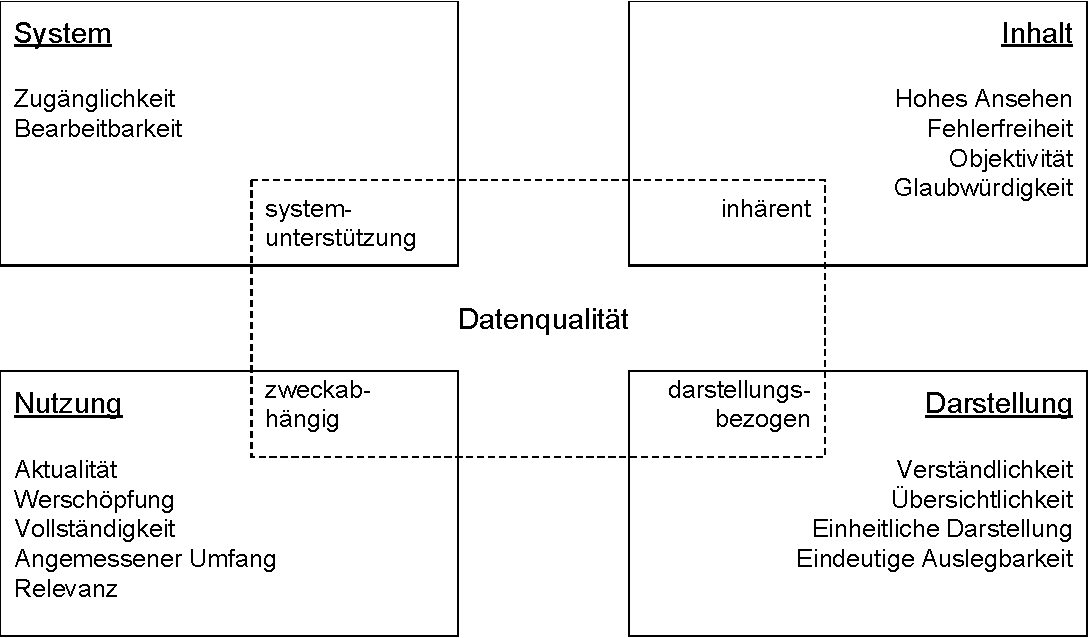
\includegraphics[scale=0.60]{content/figures/15-dimensions}
    \caption[Datenqualitätsdimensionen]{Datenqualitätsdimensionen angelehnt an~\textsc{\citeauthor{rohweder2015informationsqualitat}} (\citeyear{rohweder2015informationsqualitat}, S. 30)}\label{15-dimensions}
  \end{figure}

	Die Stammdatenqualität lässt sich anhand von verschiedenen
	Qualitätsdimensionen genauer spezifizieren.
	\textsc{\citeauthor{pipino2002data}} nennen \zB{} \textit{Fehlerfreiheit},
	\textit{Vollständigkeit}, \textit{Konsistenz}, \textit{prägnante
	Darstellung}, \textit{Relevanz}, \textit{Veränderbarkeit},
	\textit{Glaubhaftigkeit} und \textit{Aktualität} als mögliche
	Dimensionen~(\citeyear{pipino2002data, legner2007stammdaten}, S. 213 f., S. 4
	f.). \textsc{\citeauthor{baghi2013controlling}} hingegen nutzen für ihre
	Fallstudie lediglich die Datenqualitätsdimensionen \textit{Genauigkeit} und
	\textit{Vollständigkeit}~(\citeyear{baghi2013controlling}, S. 4), basierend
	auf der Erhebung von
	\textsc{\citeauthor{wand1996anchoring}} (\citeyear{wand1996anchoring}, S. 8
	f.). Die \acrlong{DGIQ} (\acrshort{DGIQ}) teilt Datenqualitätsdimensionen in
	die vier Kategorien \textit{Nutzung}, \textit{System}, \textit{Darstellung}
	und \textit{Inhalt} ein~\cite[][S. 29 ff.]{rohweder2015informationsqualitat},
	welche jeweils den Betrachtungsraum der Dimensionen abbilden (Siehe
	Abbildung~\ref{15-dimensions}).

	\subsection{Messung und Verbesserung von Stammdatenqualität}
	\textsc{\citeauthor{baghi2013controlling}} halten fest, dass Datenqualität
	nur verbessert werden kann, wenn diese dauerhaft gemessen und überwacht
	wird~(\citeyear{baghi2013controlling}, S. 2). Diese Messung kann anhand von
	Datenqualitätskennzahlen vollzogen werden, welche die Position eines
	Stammdatums in einer Datenqualitätsdimension bestimmen. Die
	Datenqualitätskennzahl \textit{nicht-leer} prüft \zB{} ob ein bestimmtes Feld
	eines Stammdatums gefüllt ist. Angewandt auf die Datenqualitätsdimension
	\textit{Vollständigkeit} der Dimensionskategorie \textit{Nutzung} kann sie
	angeben, wie vollständig ein bestimmtes Datum ist. Die Überwachung der
	Stammdatenqualität eines Unternehmens kann nach der Spezifikation von
	Datenqualitätskennzahlen von einer Stammdatenmanagement-Software, wie \zB{}
	\textit{DataRocket}, kontinuierlich auf die gesamten Stammdaten eines
	Unternehmens angewandt werden, womit nach
	\textsc{\citeauthor{baghi2013controlling}} das Fundament für die
	Datenqualitätsverbesserung erstellt ist~(\citeyear{baghi2013controlling}, S.
	2).

	Sind Qualitätsmisstände mit Hilfe von Kennzahlen ermittelt worden gilt es die
	vorhandenen Fehler zu beseitigen und deren Ursache zu identifizieren, um
	zukünftige Fehler vermeiden zu können~\cite[][S. 22]{eckerson2002data}. Ein
	Beispiel für einen Datenqualitätsmisstand ist das Fehlen der Postleitzahl in
	einer Adresse eines Kundenstammdatums. Schritt eins ist es den
	Kundendatensatz um die fehlende Postleitzahl zu erweitern. Wird in der
	Kundendateneingabemaske die Postleitzahl als Pflichtfeld deklariert wird
	dieser Fehler in der Zukunft für weitere Datensätze verhindert, womit auch
	Schritt zwei erfüllt ist.


  \subsection{Stammdatenmanagement-Software}

  \textsc{\citeauthor{baghi2014toward}} definieren
  Stammdatenmanagement-Software allgemein als eine Applikation, welche
  Attribute von Stammdaten erstellen, speichern und verändern
  kann~(\citeyear{baghi2014toward}, S. 3828). \todo{Direkt übersetzt!
  Anführungszeichen?} Sie ermöglicht es dem Endnutzer, die Daten in einer
  qualitativ hochwertigen konsolidierten Form zu konsumieren~\cite[][Abschnitt
  1.2.]{dreibelbis2008enterprise}.  \textsc{\citeauthor{baghi2014toward}}
  unterscheiden Stammdatenmanagement-Software anhand ihrer Architektur in
  \textit{Central-System}, \textit{Leading-System},
  \textit{Service-Oriented-Architecture}, \textit{Registry},
  \textit{Consolidation-Hub} und
  \textit{Peer-to-Peer}~(\citeyear{baghi2014toward}, S. 3829)~\cite[][Abschnitt
  5.3.1.]{dreibelbis2008enterprise}. Im späteren Verlauf dieser Arbeit wird auf
  die Architektur \textit{Leading-System} und \textit{Consolidation-Hub}
  verwiesen, weshalb diese Architekturen in dem nächsten Abschnitt näher
  erläutert werden.

  Im Ansatz der \textit{Leading-System}-Architektur wird für jede
  Stammdatenklasse ein System ausgewählt, \zB{} das \acrshort{CRM} für die
  Klasse der Kundendaten, welches die Hauptverwaltung dieser Klasse übernimmt,
  andere Systeme erhalten ihre Informationen über die Stammdatenklasse vom
  Hauptsystem~\cite[][S. 3829]{baghi2014toward}. Der Architekturansatz
  \textit{Consolidation-Hub} nach \textsc{\citeauthor{baghi2014toward}}
  beschreibt ein zentrales System, welches verschiedenste andere Systeme und
  Datenbanken anbindet, die Daten aus diesen verarbeitet und eine konsolidierte
  Version zur Verfügung stellt~(\citeyear{baghi2014toward}, S. 3829).
  \textsc{\citeauthor{loshin2010master}} definiert Stammdatenmanagementsoftware
  im Allgemeinen ähnlich zum
  \textit{Consolidation-Hub}~(\citeyear{loshin2010master}, S. 8). Auf die
  übrigen Architekturen wird im weiteren Verlauf der Arbeit nicht eingegangen,
  weshalb ihre Erklärungen auch nicht Teil dieser Arbeit sind. Hier wird
  lediglich auf die Erklärungen von~\textsc{\citeauthor{baghi2014toward}}
  \citeyearpar{baghi2014toward} verwiesen.


  \subsection{Vorstellung \textit{DataRocket}}\label{sec:Vorstellung-DataRocket}

	Das Unternehmen \textit{innoscale AG} entwickelt seit dem Jahr 2013
	\textit{DataRocket}, eine innovative Stammdatenmanagement-Software.
	Architektonisch verfolgt sie den Ansatz des
	\textit{Consolidation-Hubs}~\cite[][]{baghi2014toward}, indem es
	verschiedenste Informationssysteme eines Unternehmens anbindet, deren Daten
	strukturiert extrahiert und diese analysiert und in ihrer Qualität überwacht
	und verbessert. \textit{DataRocket} kann auch mit
	\textit{Leading-Systems}~\cite[][]{baghi2014toward} kollaborieren, da es
	Änderungen an Attributen eines Stammdatums an diese weiter geben kann, \bzw{}
	die Änderungen zurückschreiben kann.  Alleinstellungsmerkmale der Software
	sind: Domänenunabhängigkeit, einfache Bedienung und hoher
	Funktionsumfang\todo{\ggf{} hoher Funktionsumfang noch ersetzen}.
	\textit{DataRocket} fällt in die Gruppe der \acrshort{OLAP}-Systeme und
	implementiert einen \textit{\acrlong{ETL}}-Prozess\footnote{Für Definitionen
	des ETL-Prozesses siehe~\textsc{\citeauthor{vassiliadis2002conceptual}}
	\citeyearpar{vassiliadis2002conceptual}
	und~\textsc{\citeauthor{trujillo2003uml}}}.

	Für die Anwendung von \textit{DataRocket} auf die Stammdatenlandschaft eines
	Unternehmens wird eine Methode vorgegeben, welche im Folgenden anhand ihrer
	Schritte näher erläutert wird:

	\begin{enumerate}
		\item Eine Aggregations-Modellierung wird durchgeführt, indem so genannte
		Geschäftsobjekte\footnote{Der DataRocket-Begriff Geschäftsobjekt wird in
		Abschnitt~\ref{subsec:dimension} erläutert.} und ihre Attribute definiert
		werden und mit einander in Beziehung gebracht werden. In späteren Schritten
		wird ein solches Geschäftsobjekt mit Informationen aus verschiedenen
		Datenquellen befüllt, womit es eine Aggregation dieser darstellt. Ein
		Beispiel ist das Geschäftsobjekt \textit{Kunde}, welches die Attribute
		\textit{Name} und \textit{E-Mail-Adresse} hat. Zusätzlich besitzt es eine
		Beziehung zum Geschäftsobjekt \textit{Mitarbeiter}. 

    \item Eine Ist-Modellierung wird erstellt, indem verschiedenste
      Informationssysteme eines Unternehmens an \textit{DataRocket} angebunden
      werden und deren Struktur entweder automatisiert, oder manuell in der
			Software übernommen werden. Ein Beispiel für ein solches
			Informationssystem ist eine \textit{SQL}-Datenbank. \textit{DataRocket}
			kann das Schema der Datenbank auslesen und automatisiert ein passendes
			\textit{\acrshort{ER}}-ähnliches Modell erstellen.

		\item Die Aggregations-Modellierung wird der Ist-Modellierung zugeordnet,
		indem Geschäftsobjekte beider Welten miteinander verbunden werden. Im
		Kontext des oben genannten Beispiels wird hier das \acrshort{CRM}-System
		eines Unternehmens mit \textit{DataRocket} verbunden und die Attribute des
		Geschäftsobjekt \textit{Kunde} des \acrshort{CRM}-Systems dem
		Geschäftsobjekt \textit{Kunde} der Aggregations-Modellierung zugewiesen.
		Kommt dieser Prozess \zB{} im Rahmen einer Umstrukturierungsmaßnahme
		zum Einsatz, so kann die Aggregations- und Ist-Modellierung mit der Soll-
		und Ist-Modellierung nach \textsc{\citeauthor{becker2006konzeptionelle}}
		verglichen werden~(\citeyear{becker2006konzeptionelle}, S. 3).

		\item Qualitätskennzahlen werden für Attribute von Geschäftsobjekten
		definiert, indem entweder auf einen bereitgestellten Katalog von
		Auswertungsfunktionen zurückgegriffen wird, oder eigene Attribute durch die
		Formulierung von regulären Ausdrücken erstellt werden. Ein Beispiel einer
		Qualitätskennzahl für das Geschäftsobjekt \textit{Kunde} ist eine Kennzahl,
		welche überprüft, ob das Attribut \textit{E-Mail-Adresse} des
		Geschäftsobjekts ein At-Zeichen enthält.

		\item Aggregierte Instanzen eines zuvor modellierten Geschäftsobjekts
		werden im \textit{DataRocket} \textit{Instance-Loader}-Baustein geladen.
		Hierzu spezifiziert der Nutzer das gewünschte Geschäftsobjekt, welches er
		im weiteren Verlauf analysieren möchte, und die angebunden Datenquellen,
		aus welchen er die Instanzen laden möchte.

		\item Die Instanzen der Geschäftsobjekte werden mit Hilfe der zuvor
		spezifizierten Qualitätskennzahlen im sogenannten
		\textit{Calculation}-Baustein analysiert. In diesem Baustein wählt der
		Nutzer zunächst die Kennzahlen aus, welche im folgenden Schritt auf die
		Geschäftsobjektinstanzen angewendet werden. Die Auswertungsergebnisse
		einzelner Instanzen werden anhand von Geschäftsobjektinstanzaggregationen
		gruppiert. Ein mögliches Auswertungsergebnis für das gesamte
		Geschäftsobjekt Kunde über alle Instanzen ist, dass vier Prozent aller
		Kundenstammdaten in dem Attribut \textit{E-Mail-Adresse} das At-Zeichen
		fehlt.

		\item Die Ergebnisse der Geschäftsobjektanalyse können mit Hilfe von
		verschiedenen Diagrammen, wie \zB{} einem Linien- oder Säulendiagramm, im
		\textit{Visualization}-Baustein optisch aufbereitet werden. Diese können in
		der Berichterstattungskomponente aufgegriffen werden, welche nachfolgend
		genauer beschrieben wird.

		\item Datenqualitätsprobleme können manuell oder automatisiert im
		\textit{Cleaning}-Baustein behoben werden. Für die manuelle Behebung werden
		dem Nutzer nacheinander Geschäftsobjekte mit Datenqualitätsproblemen
		angezeigt, welche er direkt in der Software bereinigen kann. Für die
		automatisierte Behebung bietet \textit{DataRocket} verschieden Module. Ein
		Beispiel\-modul dient der Bereinigung von Adressdaten. Hierzu werden
		externe Geo- und Adressdatenbanken wie \zB{} \textit{Google Maps},
		\textit{Melissa Data} oder \textit{Kreditreform} angebunden, welche
		\textit{DataRocket} mit den Adressdaten der Geschäftsobjektinstanzen
		vergleicht und diese hiermit \ggf{} ergänzt oder korrigiert. Die
		Datenänderungen können von \textit{DataRocket} automatisiert in das
		Informationsquellsystem zurückgeschrieben werden.

    \item \textit{DataRocket} überwacht alle angebundenen Datenquellen
      kontinuierlich und bietet in der Benutzerschnittstelle eine
      Berichterstattungskomponente, welche dem User sowohl den aktuellen Status
      quo der Datenqualität im Unternehmen, als auch die Entwicklung im
      Zeitverlauf anzeigt.
	\end{enumerate}

	Der sequentielle Prozess, beschrieben in den Schritten fünf bis acht und in Abbildung~\ref{fig:datapipeline}, wird in
	der Benutzeroberfläche durch das Modul \textit{DataPipeline} abgebildet.
	Diese ermöglicht es dem Nutzer verschiedene Prozessschritte wie Bausteine
	aneinanderzureihen, welche jeweils auf die Ausgabewerte ihrer Vorgänger als
	eigene Eingabewerte aufbauen. Sie ist vergleichbar mit dem
	\textit{Pipeline}-Pattern des Software-Engineerings, wie \zB{} der
	\textit{Pipeline} in Unix-ähnlichen
	Betriebssystemen~\cite[][]{spinellis2001notable}. Im bisherigen
	Beispielszenario würde zunächst das Geschäftsobjekt \textit{Kunde} im
	\textit{Instance-Loader}-Baustein geladen werden und mit Hilfe der zuvor
	definierten Qualitätskennzahlen im \textit{Calculation}-Baustein analysiert
	werden. Die Ergebnisse der Analyse werden weiter an den
	\textit{Visualization}-Baustein gegeben, welcher diese in Form von Graphen
	darstellt. Abschließend greift der \textit{Cleaning}-Baustein auf die
	Ergebnisse zu, in welchem der User die zuvor festgestellten
	Datenqualitätsprobleme beheben kann.

  \begin{figure}
    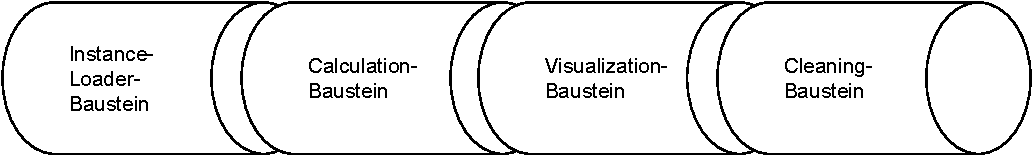
\includegraphics[scale=0.9]{content/figures/datapipeline}
    \caption{\textit{DataRocket} \textit{DataPipeline}}\label{fig:datapipeline}
  \end{figure}


	Ziel dieser Arbeit ist die Spezifikation einer Datenanalysesprache und die
	prototypische Entwicklung einer Komponente, \textit{DataFurnace}, für
	\textit{DataRocket}. Sowohl die Sprache als auch die Komponente sollen im
	\textit{Calculation}-Baustein der \textit{Datapipeline} Anwendung finden.

  \section{Anwendungsfallbeispiel}\label{sec:anwendungsfallbeispiel}

  Für den weiteren Verlauf dieser Arbeit wird ein Anwendungsbeispiel
  aufgestellt, auf welches in Erklärungen der \textit{DataFurnace}-Sprache und
  -Software zurückgegriffen wird. Im Fokus steht ein fiktives
  Einzelhandelsgeschäft, welches auf den Verkauf von Lebensmitteln
  spezialisiert ist, jedoch auch andere Produkte des täglichen Bedarfs
  verkauft. Das Unternehmen betreibt zwei Standorte, jeweils in den Städten
  Münster und Bonn.

  Lebensmittel haben ein Mindesthaltbarkeitsdatum und dürfen bei dessen
  Überschreitung nicht verkauft werden. Um zu verhindern, dass Handelsware
  abläuft, sollen möglichst alle Lebensmittel vor ihrem
  Mindesthaltbarkeitsdatum verkauft werden. Eine kontinuierliche
  Marketingkampagne soll Anreize zum Kauf von Lebensmitteln setzen, welche
  innnerhalb des kommenden Monats ablaufen. Diese Anreize sollen in Form von
  Rabatten auf diese Produkte realisiert werden. Um Aufmerksamkeit für die
  Kampagne zu erhalten, sollen die Rabatte einmal im Monat per E-Mail oder Post
  beworben werden. 

  Bevor die Marketingkampagne geplant und ausgeführt werden kann, muss zunächst
  ihre Durchführbarkeit geprüft werden. Sie beruht maßgeblich auf der
  Datenqualität der Produktdaten im \acrlong{WWS} (\acrshort{WWS}) und den
  Kundendaten im \acrlong{CRM}-Systems (\acrshort{CRM}) des Unternehmens. Die
  Datenstrukturen der Stammdatensätze werden in
  Abbildung~\ref{example-use-case-data} durch ein UML-Klassendiagramm
  beschrieben. Im Folgenden werden Fragestellungen, welche für die
  Durchführbarkeitsanalyse der Marketingkampagne beantwortet werden müssen, und
  deren Bedingungen aufgelistet.

  \begin{figure}
    \resizebox{250pt}{!}{% Graphic for TeX using PGF
% Title: /home/indenml/code/bachelor_thesis/content/figures/example-use-case-data.dia
% Creator: Dia v0.97.3
% CreationDate: Sun Sep 11 16:45:34 2016
% For: indenml
% \usepackage{tikz}
% The following commands are not supported in PSTricks at present
% We define them conditionally, so when they are implemented,
% this pgf file will use them.
\ifx\du\undefined{}
  \newlength{\du}
\fi
\setlength{\du}{15\unitlength}
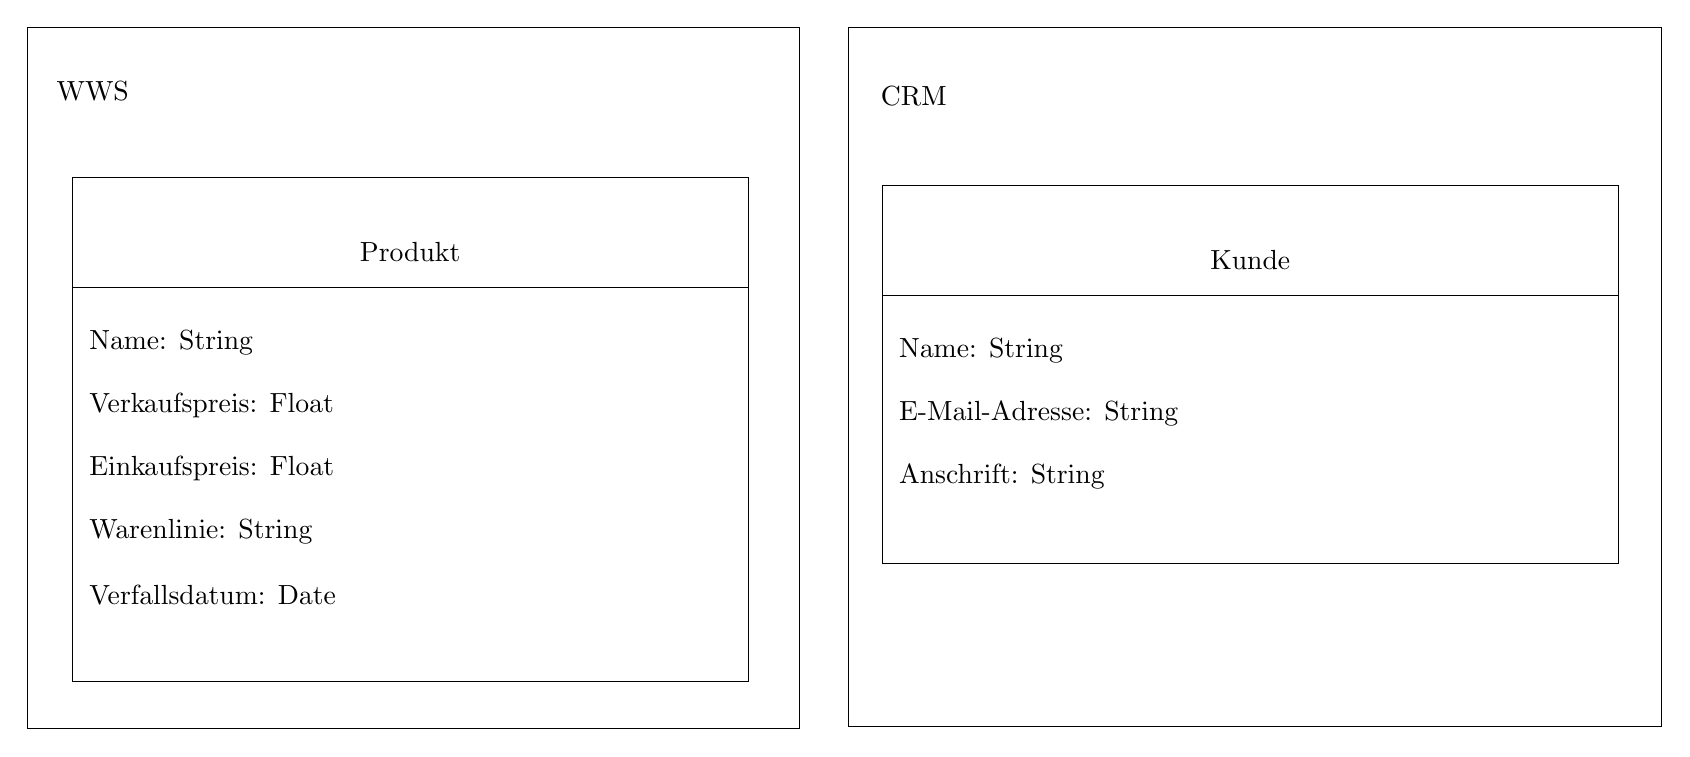
\begin{tikzpicture}
\pgftransformxscale{1.000000}
\pgftransformyscale{-1.000000}
\definecolor{dialinecolor}{rgb}{0.000000, 0.000000, 0.000000}
\pgfsetstrokecolor{dialinecolor}
\definecolor{dialinecolor}{rgb}{1.000000, 1.000000, 1.000000}
\pgfsetfillcolor{dialinecolor}
\pgfsetlinewidth{0.000000\du}
\pgfsetdash{{1.000000\du}{1.000000\du}}{0\du}
\pgfsetdash{{0.300000\du}{0.300000\du}}{0\du}
\pgfsetmiterjoin
\definecolor{dialinecolor}{rgb}{1.000000, 1.000000, 1.000000}
\pgfsetfillcolor{dialinecolor}
\fill (0.600000\du,4.150000\du)--(0.600000\du,13.050000\du)--(10.400000\du,13.050000\du)--(10.400000\du,4.150000\du)--cycle;
\definecolor{dialinecolor}{rgb}{0.000000, 0.000000, 0.000000}
\pgfsetstrokecolor{dialinecolor}
\draw (0.600000\du,4.150000\du)--(0.600000\du,13.050000\du)--(10.400000\du,13.050000\du)--(10.400000\du,4.150000\du)--cycle;
\pgfsetlinewidth{0.000000\du}
\pgfsetdash{}{0pt}
\definecolor{dialinecolor}{rgb}{1.000000, 1.000000, 1.000000}
\pgfsetfillcolor{dialinecolor}
\fill (1.165000\du,6.050000\du)--(1.165000\du,7.450000\du)--(9.750000\du,7.450000\du)--(9.750000\du,6.050000\du)--cycle;
\definecolor{dialinecolor}{rgb}{0.000000, 0.000000, 0.000000}
\pgfsetstrokecolor{dialinecolor}
\draw (1.165000\du,6.050000\du)--(1.165000\du,7.450000\du)--(9.750000\du,7.450000\du)--(9.750000\du,6.050000\du)--cycle;
% setfont left to latex
\definecolor{dialinecolor}{rgb}{0.000000, 0.000000, 0.000000}
\pgfsetstrokecolor{dialinecolor}
\node at (5.457500\du,7.000000\du){Produkt};
\definecolor{dialinecolor}{rgb}{1.000000, 1.000000, 1.000000}
\pgfsetfillcolor{dialinecolor}
\fill (1.165000\du,7.450000\du)--(1.165000\du,12.450000\du)--(9.750000\du,12.450000\du)--(9.750000\du,7.450000\du)--cycle;
\definecolor{dialinecolor}{rgb}{0.000000, 0.000000, 0.000000}
\pgfsetstrokecolor{dialinecolor}
\draw (1.165000\du,7.450000\du)--(1.165000\du,12.450000\du)--(9.750000\du,12.450000\du)--(9.750000\du,7.450000\du)--cycle;
% setfont left to latex
\definecolor{dialinecolor}{rgb}{0.000000, 0.000000, 0.000000}
\pgfsetstrokecolor{dialinecolor}
\node[anchor=west] at (1.265000\du,8.150000\du){Name: String};
% setfont left to latex
\definecolor{dialinecolor}{rgb}{0.000000, 0.000000, 0.000000}
\pgfsetstrokecolor{dialinecolor}
\node[anchor=west] at (1.265000\du,8.950000\du){Verkaufspreis: Float};
% setfont left to latex
\definecolor{dialinecolor}{rgb}{0.000000, 0.000000, 0.000000}
\pgfsetstrokecolor{dialinecolor}
\node[anchor=west] at (1.265000\du,9.750000\du){Einkaufspreis: Float};
% setfont left to latex
\definecolor{dialinecolor}{rgb}{0.000000, 0.000000, 0.000000}
\pgfsetstrokecolor{dialinecolor}
\node[anchor=west] at (1.265000\du,10.550000\du){Warenlinie: String};
% setfont left to latex
\definecolor{dialinecolor}{rgb}{0.000000, 0.000000, 0.000000}
\pgfsetstrokecolor{dialinecolor}
\node[anchor=west] at (1.265000\du,11.350000\du){Verfallsdatum: Date};
% setfont left to latex
\definecolor{dialinecolor}{rgb}{0.000000, 0.000000, 0.000000}
\pgfsetstrokecolor{dialinecolor}
\node[anchor=west] at (1.265000\du,12.150000\du){};
% setfont left to latex
\definecolor{dialinecolor}{rgb}{0.000000, 0.000000, 0.000000}
\pgfsetstrokecolor{dialinecolor}
\node[anchor=west] at (0.850000\du,4.950000\du){WWS};
\pgfsetlinewidth{0.000000\du}
\pgfsetdash{{0.300000\du}{0.300000\du}}{0\du}
\pgfsetdash{{0.300000\du}{0.300000\du}}{0\du}
\pgfsetmiterjoin
\definecolor{dialinecolor}{rgb}{1.000000, 1.000000, 1.000000}
\pgfsetfillcolor{dialinecolor}
\fill (11.020000\du,4.150000\du)--(11.020000\du,13.025000\du)--(21.350000\du,13.025000\du)--(21.350000\du,4.150000\du)--cycle;
\definecolor{dialinecolor}{rgb}{0.000000, 0.000000, 0.000000}
\pgfsetstrokecolor{dialinecolor}
\draw (11.020000\du,4.150000\du)--(11.020000\du,13.025000\du)--(21.350000\du,13.025000\du)--(21.350000\du,4.150000\du)--cycle;
\pgfsetlinewidth{0.000000\du}
\pgfsetdash{}{0pt}
\definecolor{dialinecolor}{rgb}{1.000000, 1.000000, 1.000000}
\pgfsetfillcolor{dialinecolor}
\fill (11.450000\du,6.150000\du)--(11.450000\du,7.550000\du)--(20.805000\du,7.550000\du)--(20.805000\du,6.150000\du)--cycle;
\definecolor{dialinecolor}{rgb}{0.000000, 0.000000, 0.000000}
\pgfsetstrokecolor{dialinecolor}
\draw (11.450000\du,6.150000\du)--(11.450000\du,7.550000\du)--(20.805000\du,7.550000\du)--(20.805000\du,6.150000\du)--cycle;
% setfont left to latex
\definecolor{dialinecolor}{rgb}{0.000000, 0.000000, 0.000000}
\pgfsetstrokecolor{dialinecolor}
\node at (16.127500\du,7.100000\du){Kunde};
\definecolor{dialinecolor}{rgb}{1.000000, 1.000000, 1.000000}
\pgfsetfillcolor{dialinecolor}
\fill (11.450000\du,7.550000\du)--(11.450000\du,10.950000\du)--(20.805000\du,10.950000\du)--(20.805000\du,7.550000\du)--cycle;
\definecolor{dialinecolor}{rgb}{0.000000, 0.000000, 0.000000}
\pgfsetstrokecolor{dialinecolor}
\draw (11.450000\du,7.550000\du)--(11.450000\du,10.950000\du)--(20.805000\du,10.950000\du)--(20.805000\du,7.550000\du)--cycle;
% setfont left to latex
\definecolor{dialinecolor}{rgb}{0.000000, 0.000000, 0.000000}
\pgfsetstrokecolor{dialinecolor}
\node[anchor=west] at (11.550000\du,8.250000\du){Name: String};
% setfont left to latex
\definecolor{dialinecolor}{rgb}{0.000000, 0.000000, 0.000000}
\pgfsetstrokecolor{dialinecolor}
\node[anchor=west] at (11.550000\du,9.050000\du){E-Mail-Adresse: String};
% setfont left to latex
\definecolor{dialinecolor}{rgb}{0.000000, 0.000000, 0.000000}
\pgfsetstrokecolor{dialinecolor}
\node[anchor=west] at (11.550000\du,9.850000\du){Anschrift: String};
% setfont left to latex
\definecolor{dialinecolor}{rgb}{0.000000, 0.000000, 0.000000}
\pgfsetstrokecolor{dialinecolor}
\node[anchor=west] at (11.550000\du,10.650000\du){};
\definecolor{dialinecolor}{rgb}{1.000000, 1.000000, 1.000000}
\pgfsetfillcolor{dialinecolor}
\fill (11.320000\du,4.425000\du)--(11.320000\du,5.170000\du)--(12.920000\du,5.170000\du)--(12.920000\du,4.425000\du)--cycle;
% setfont left to latex
\definecolor{dialinecolor}{rgb}{0.000000, 0.000000, 0.000000}
\pgfsetstrokecolor{dialinecolor}
\node[anchor=west] at (11.320000\du,5.020000\du){CRM};
\end{tikzpicture}
}
    \caption{Datenstruktur des Produkt- und Kundenstammdatensatzes}\label{example-use-case-data}
  \end{figure}

  \begin{itemize}

    \item Der Rabatt soll nicht nur in relativen, sondern auch absoluten Zahlen
      beworben werden. Folglich muss im Warenwirtschaftssystem ein valider
      Preis für jedes zu bewerbende Produkt vorliegen. Es wird angenommen, dass
      die Attribute \textit{Verkaufspreis} und \textit{Einkaufspreis} in
      Eurocent angegeben werden.

    \item Es soll zunächst eine Pilotkampagne an einem der beiden Standorte im
      nächsten (Oktober) oder übernächsten (November) Monat gestartet werden.
      Für diese Kampagne soll die Standort-Monat-Kombination gewählt werden,
      bei welcher ohne die Kampagne der größte Gewinnverlust durch abgelaufene
      Produkte entstehen würde.

    \item Die Kampagne kann entweder per E-Mail oder per Post beworben werden.
      Nun stellt sich die Frage, für wie viele Kunden im \acrshort{CRM}-System
      eine E-Mail-Adresse und für wie viele eine Postanschrift hinterlegt ist.

    \item Das \textit{CRM}-System des Unternehmens enthält viele Karteileichen.
      Um die Ausschöpfungsquote hoch zu halten, sollen nur die Kunden
      betrachtet werden, welche innerhalb dieses Jahres zuletzt eingekauft
      haben.

  \end{itemize}

  Um diese Fragestellungen unter der Beachtung der Bedingungen beantworten zu
  können, müssen die Kunden- und Produktstammdaten des Unternehmens analysiert
  werden. Der erste Schritt im Rahmen dieser Auswertung ist die Modellierung
  der Analyse \zB{} mit der \textit{DataFurnace}-Sprache und -Software.

  % ################################################################################
  \chapter{Entwicklung der \textit{DataFurnace}-Sprache}\label{ch:entwicklung-datafurnace-sprache}
  % ################################################################################

  \todo[inline]{Theorie / Vorgehensmodell für die Entwicklung von Sprachen?}


  \section{Motivation}

	Die Stammdatenmanagement-Software \textit{DataRocket} muss im Rahmen der
	Datenqualitätsver\-besserung die Qualität von Unternehmensdaten zunächst
	untersuchen. Der \textit{DataRocket}-Nutzer muss hierzu \textit{DataRocket}
	genau anweisen, nach welchen Kriterien er Datenqualität definiert und wie die
	Daten anhand der Datenqualitätsdefinitionen analysiert werden sollen. Für die
	Kommunikation zwischen \textit{DataRocket} und Nutzer ist folglich eine
	Sprache von Nöten, welche es dem Nutzer ermöglicht, \textit{DataRocket} die
	funktionale Struktur der zu analysiereden Daten zu erklären,
	Qualitätskriterien zu definieren und Analyseziele zu spezifizieren.
	Gegenstandsbe\-reich der Sprache ist der Einsatz in \textit{DataRocket} im
	\textit{Calculation}-Baustein der \textit{DataPipeline} aus
	Abschnitt~\ref{sec:Vorstellung-DataRocket}.


  \section{Anforderungsanalyse und Annahmen}\label{sec:sprache/anforderungsanalyse}

	Im Folgenden wird eine Anforderungsanalyse für die
	\textit{DataFurnace}-Sprache durchgeführt, um genaue Anforderungen an die
	Sprache für die spätere Entwicklung dieser zu sammeln und zu spezifizieren.
	Hierzu wird auf die Vorgehensweise der \textit{zielorientierten
	Anforderungsanalyse} zurückgegriffen, näher beschrieben von
	\textsc{\citeauthor{van2001goal}}~\citeyearpar{van2001goal}.  Ziele werden
	unterschieden in \textit{funktionale} und \textit{nicht-funktionale}
	Ziele~\cite[][S.  36]{mylopoulos1999object}.  Erstere beschreiben die
	Leistungen der Sprache selbst, zweitere beschäftigen sich mit der Art und
	Weise respektive mit der Qualität der Leistung~\cite[][S.  250]{van2001goal}.
	Die Ziele der \textit{DataFurnace}-Sprache werden in den folgenden
	Aufzählungen benannt, näher beschrieben und begründet.

  \paragraph{Funktionale Ziele}
    \begin{enumerate}
      \item \textbf{Spezifikation der Unternehmensdatenstrukturen} 

        Unternehemensdatentypen sollen in ihrem Aufbau spezifiziert werden
        können. Hierzu zählt die Benennung von Attributen eines Datensatztypus
        und die Spezifikation der hierarchischen Strukturen innerhalb seiner
        Attribute. Zum Beispiel soll dem Unternehmensdatentyp \textit{Produkt}
        die Attribute \textit{Preis} und \textit{Produktkategorie} zugeordnet
        werden können. Das Attribut \textit{Produktkategorie} soll des Weiteren
        in seine Bestandteile \textit{Warenlinie} und \textit{Warenbereich}
        aufgeteilt werden können, wobei der Nutzer die Möglichkeit haben soll,
        den Warenbereich der Warenlinie funktional unterzuordnen.

      \item \textbf{Definition von Kennzahlen} 

        \textit{DataRocket} misst Datenqualität anhand von
        Datenqualtitätskennzahlen. Ziel ist es, diese mit Hilfe der
        \textit{DataFurnace}-Sprache definieren zu können.
        Datenqualitätskennzahlen beziehen sich auf Attribute von
        Unternehmensdatentypen. Die Sprache soll es dem Nutzer ermöglichen,
        komplizierte Qualitätskennzahlberechnungen zu spezifizieren. Es
        soll zum Beispiel eine Qualtitätskennzahl definiert werden können,
        welche kontrolliert, dass im oben genannten Szenario der \textit{Preis}
        des Unternehmensdatentypus \textit{Produkt} keine Buchstaben enthält.

        Um im späteren Bericht nicht nur nach Datenqualitätsmerkmalen filtern
        zu können, sollen die \textit{DataFurnace}-Kennzahlen so allgemein
        gehalten werden, dass sie nicht nur der Datenqualitätsbeurteilung
        dienen, sondern auch allgemeine Beurteilungen erbringen können. Will
        sich ein Nutzer beispielsweise in einem großen Datenqualitätsprojekt
        zunächst nur auf die lukrativen Instanzen des Geschäftsobjekt
        \textit{Produkt} konzentrieren, so soll er mit Hilfe der
        betriebswirtschaftlichen Kennzahl \textit{Gewinn} diese gefiltert
        analysieren können.
        
      \item \textbf{Kombination zu Berichten}

        Ein Nutzer soll die Kombination von zuvor spezifizierten
        Unternehmensdaten mit den definierten Datenqualtiätskennzahlen zu
        verschiedensten Auswertungsszenarien mit Hilfe der Sprache beschreiben
        können. Somit soll es die Sprache ermöglichen, Fragestellungen zu
        entwickeln, welche die Qualtität von bestimmten Datensätzen hinterfragen.
        Zusätzlich soll sie den Nutzer befähigen, innerhalb einer
        Fragestellung, mit Hilfe von Attributen, Datensätze gefiltert zu
        betrachten und anhand von Attributgruppen zu vergleichen. Eine mögliche
        Fragestellung im oben aufgespannten Szenario ist: Wie viele
        \textit{Produkte} in der \textit{Warenlinie} \textit{Elektronik} haben
        im Vergleich zur \textit{Warenlinie} \textit{Lebenmittel} Buchstaben im
        Attribut \textit{Preis}.
    \end{enumerate}

  \paragraph{Nicht-funktionale Ziele}
    \begin{enumerate}
      \item \textbf{Hohe Verständlichkeit}

				Die Sprache soll sehr leicht verständlich sein, um mit dem
				Alleinstellungsmerkmal von \textit{DataRocket}, den Zugang zu
				Datenqualitätsmanagement IT-Laien zu ermöglichen, kohärent zu bleiben.
				Besonderer Fokus soll auf einer geringen Komplexität der Sprache
				liegen, wodurch der Nutzer die Sprache schnell verstehen und erlernen
				kann.

      \item \textbf{Verwendung des \textit{DataRocket}-Vokabulars}

				Die Software \textit{DataRocket} nutzt in ihrer Oberfläche die
				Englische Sprache zur Kommunikation mit dem Nutzer. Zusätzlich benutzt
				die Software einige Begriffe des Datenqualitätsmanagement-Jargons, wie
				\zB{} Datenqualitätskennzahl, und führt in einigen wenigen Fällen ein
				eigenes Vokabular ein, welches unikale Komponenten und Vorgänge der
				Software betitelt, wie \zB{} das Geschäftsobjekt. Zwar soll die
				\textit{DataFurnace}-Sprache und -Komponente alleinstehend entwickelt
				werden, jedoch soll bei der Entwicklung auch die zukünftige Integration
				der beiden in \textit{DataRocket} nicht unbeachtet bleiben. Folglich
				sollte sich das Vokabular der \textit{DataFurnace}-Sprache an dem
				Vokabular von \textit{DataRocket} orientieren und an den
				Funktionsschnittstellen übereinstimmen.

    \end{enumerate}

	\paragraph{Annahmen} Neben \textit{funktionalen} und
	\textit{nicht-funktionalen} Zielen müssen des Weiteren Annahmen getroffen
	werden, welche von der \textit{innoscale AG} vorrausgesetzt werden, und somit
	die Entwicklung der Sprache beeinflussen.

  \begin{enumerate}
    \item \textbf{Datentransformation durch \textit{DataRocket}}

      Im Funktionsumfang von \textit{DataRocket} ist der so genannten
      \textit{Mapper} enthalten, welcher es dem Nutzer ermöglicht, Daten in
      verschiedenste gewünschte Strukturen zu transformieren. Folglich kann für
      die Entwicklung der \textit{DataFurnace}-Sprache die Möglichkeit der
      Beschreibung einer Transformation von Datenstrukturen außer Acht gelassen
      werden, mit der Annahme, dass die \textit{DataFurnace}-Software auf die
      zuvor von \textit{DataRocket} strukturierten Daten aufbauen kann, indem
      es direkt mit Geschäftsobjekten\footnote{Der \textit{DataRocket}-Begriff
      Geschäftsobjekt wird in Abschnitt~\ref{subsec:dimension} erläutert.}
      arbeitet.

      \todo[inline]{Weitere Annahme hinzufügen}

  \end{enumerate}


  \section{Fachliches Konzept}

  Die \textit{DataFurnace}-Sprache wurde in enger Zusammenarbeit und ständiger
  Absprache mit der \textit{innoscale AG} und unter Einbeziehung des
  aktuellen Stand der Wissenschaft im Bereich des Datenqualitätsmanagements und
  der Unternehmensdatenanalyse entwickelt. Im Folgenden wird die Sprache,
  strukturiert anhand ihres Vokabulars, erklärt. Dieses unterteilt sich in die
  Vokabulargruppen Dimensionen, Kennzahlen und Berichte, welche in ihrer Summe
  die \textit{DataFurnace}-Sprache ausmachen. Die gesamte Sprache ist in
  Abbildung~\ref{fig:language_spec-erm} gezeigt, welche für jede
  Vokabulargruppe in Ausschnitten betrachtet wird.

  \begin{figure}
    \resizebox{\columnwidth}{!}{% Graphic for TeX using PGF
% Title: /home/indenml/code/bachelor_thesis/content/figures/language_spec-erm.dia
% Creator: Dia v0.97.3
% CreationDate: Tue Sep 27 11:28:12 2016
% For: indenml
% \usepackage{tikz}
% The following commands are not supported in PSTricks at present
% We define them conditionally, so when they are implemented,
% this pgf file will use them.
\ifx\du\undefined
  \newlength{\du}
\fi
\setlength{\du}{15\unitlength}
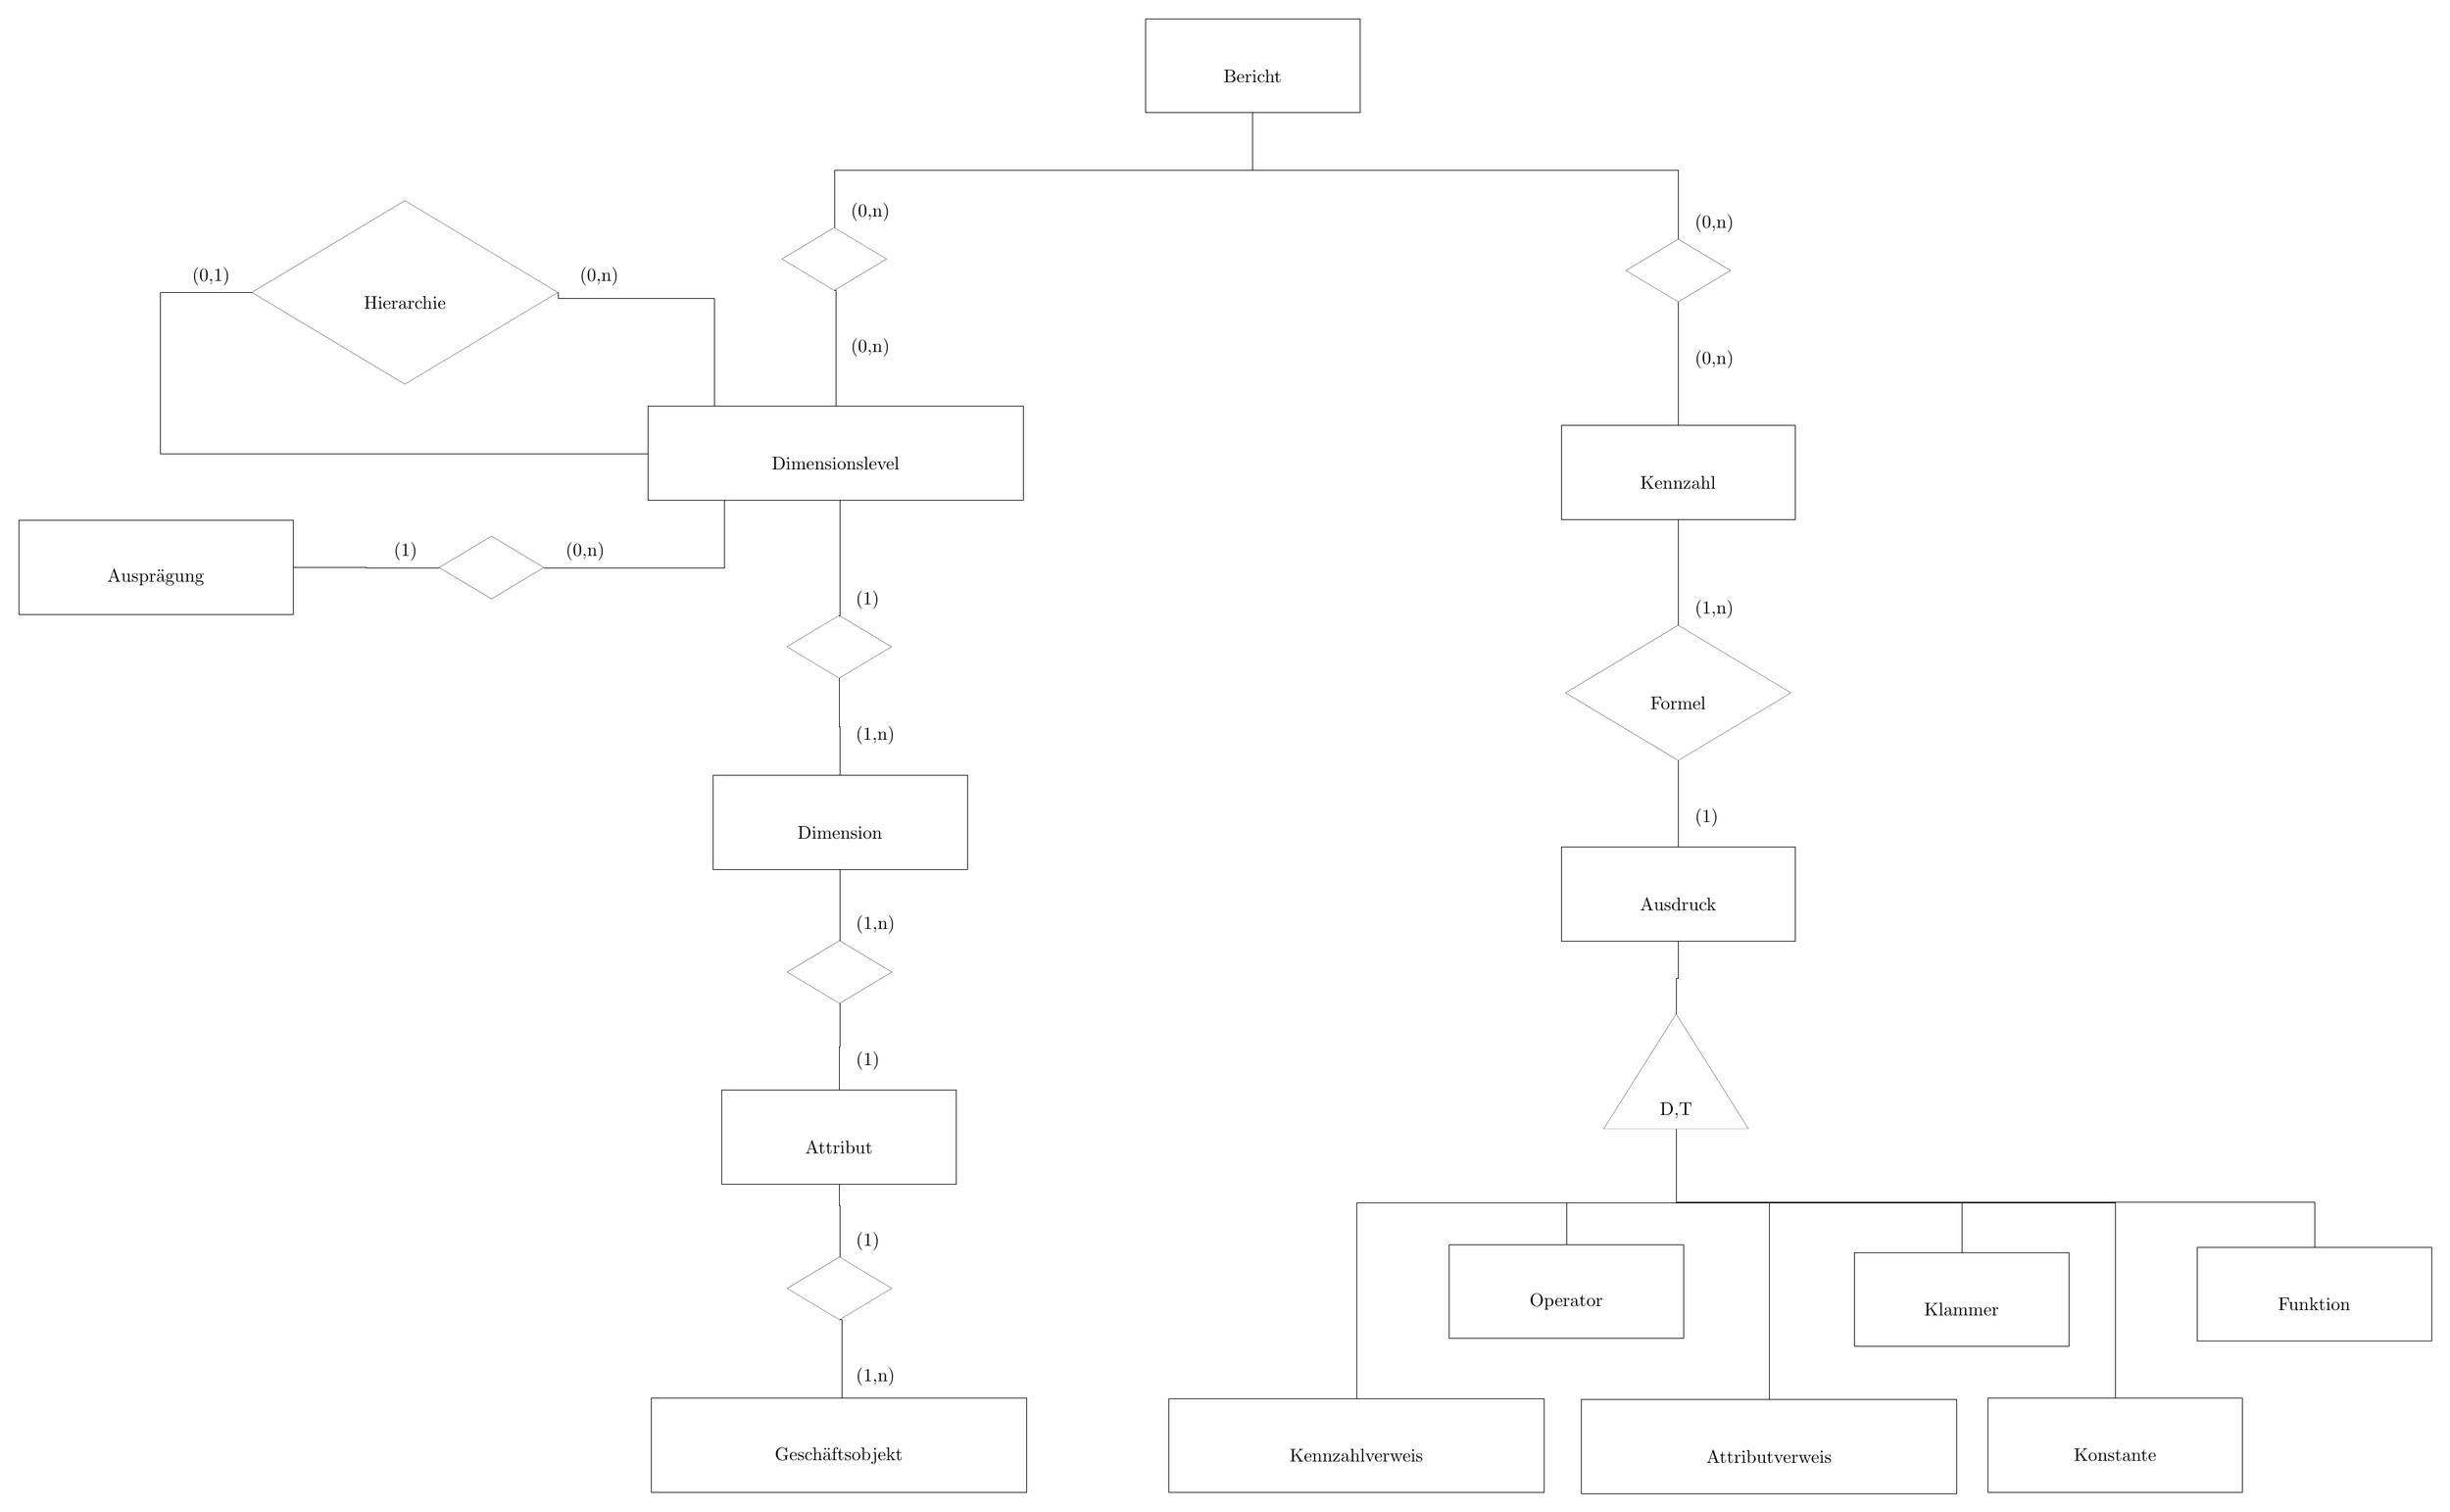
\begin{tikzpicture}
\pgftransformxscale{1.000000}
\pgftransformyscale{-1.000000}
\definecolor{dialinecolor}{rgb}{0.000000, 0.000000, 0.000000}
\pgfsetstrokecolor{dialinecolor}
\definecolor{dialinecolor}{rgb}{1.000000, 1.000000, 1.000000}
\pgfsetfillcolor{dialinecolor}
\definecolor{dialinecolor}{rgb}{1.000000, 1.000000, 1.000000}
\pgfsetfillcolor{dialinecolor}
\fill (-1.973220\du,32.336600\du)--(-1.973220\du,34.136600\du)--(2.891780\du,34.136600\du)--(2.891780\du,32.336600\du)--cycle;
\pgfsetlinewidth{0.100000\du}
\pgfsetdash{}{0pt}
\pgfsetmiterjoin
\definecolor{dialinecolor}{rgb}{0.000000, 0.000000, 0.000000}
\pgfsetstrokecolor{dialinecolor}
\draw (-1.973220\du,32.336600\du)--(-1.973220\du,34.136600\du)--(2.891780\du,34.136600\du)--(2.891780\du,32.336600\du)--cycle;
% setfont left to latex
\definecolor{dialinecolor}{rgb}{0.000000, 0.000000, 0.000000}
\pgfsetstrokecolor{dialinecolor}
\node at (0.459280\du,33.436600\du){Dimension};
\definecolor{dialinecolor}{rgb}{1.000000, 1.000000, 1.000000}
\pgfsetfillcolor{dialinecolor}
\fill (-3.210480\du,25.273700\du)--(-3.210480\du,27.073700\du)--(3.964520\du,27.073700\du)--(3.964520\du,25.273700\du)--cycle;
\pgfsetlinewidth{0.100000\du}
\pgfsetdash{}{0pt}
\pgfsetmiterjoin
\definecolor{dialinecolor}{rgb}{0.000000, 0.000000, 0.000000}
\pgfsetstrokecolor{dialinecolor}
\draw (-3.210480\du,25.273700\du)--(-3.210480\du,27.073700\du)--(3.964520\du,27.073700\du)--(3.964520\du,25.273700\du)--cycle;
% setfont left to latex
\definecolor{dialinecolor}{rgb}{0.000000, 0.000000, 0.000000}
\pgfsetstrokecolor{dialinecolor}
\node at (0.377020\du,26.373700\du){Dimensionslevel};
\definecolor{dialinecolor}{rgb}{1.000000, 1.000000, 1.000000}
\pgfsetfillcolor{dialinecolor}
\fill (-1.800000\du,38.350000\du)--(-1.800000\du,40.150000\du)--(2.680000\du,40.150000\du)--(2.680000\du,38.350000\du)--cycle;
\pgfsetlinewidth{0.100000\du}
\pgfsetdash{}{0pt}
\pgfsetmiterjoin
\definecolor{dialinecolor}{rgb}{0.000000, 0.000000, 0.000000}
\pgfsetstrokecolor{dialinecolor}
\draw (-1.800000\du,38.350000\du)--(-1.800000\du,40.150000\du)--(2.680000\du,40.150000\du)--(2.680000\du,38.350000\du)--cycle;
% setfont left to latex
\definecolor{dialinecolor}{rgb}{0.000000, 0.000000, 0.000000}
\pgfsetstrokecolor{dialinecolor}
\node at (0.440000\du,39.450000\du){Attribut};
\definecolor{dialinecolor}{rgb}{1.000000, 1.000000, 1.000000}
\pgfsetfillcolor{dialinecolor}
\fill (-10.782700\du,23.101400\du)--(-7.857700\du,21.346400\du)--(-4.932700\du,23.101400\du)--(-7.857700\du,24.856400\du)--cycle;
\pgfsetlinewidth{0.100000\du}
\pgfsetdash{}{0pt}
\pgfsetmiterjoin
\definecolor{dialinecolor}{rgb}{0.000000, 0.000000, 0.000000}
\pgfsetstrokecolor{dialinecolor}
\draw (-10.782700\du,23.101400\du)--(-7.857700\du,21.346400\du)--(-4.932700\du,23.101400\du)--(-7.857700\du,24.856400\du)--cycle;
% setfont left to latex
\definecolor{dialinecolor}{rgb}{0.000000, 0.000000, 0.000000}
\pgfsetstrokecolor{dialinecolor}
\node[anchor=east] at (-11.082700\du,22.801400\du){(0,1)};
\definecolor{dialinecolor}{rgb}{0.000000, 0.000000, 0.000000}
\pgfsetstrokecolor{dialinecolor}
\node[anchor=west] at (-4.632700\du,22.801400\du){(0,n)};
\definecolor{dialinecolor}{rgb}{0.000000, 0.000000, 0.000000}
\pgfsetstrokecolor{dialinecolor}
\node at (-7.857700\du,23.301400\du){Hierarchie};
\pgfsetlinewidth{0.100000\du}
\pgfsetdash{}{0pt}
\pgfsetmiterjoin
\pgfsetbuttcap
\definecolor{dialinecolor}{rgb}{0.000000, 0.000000, 0.000000}
\pgfsetstrokecolor{dialinecolor}
\draw (-3.210480\du,26.173700\du)--(-3.210480\du,26.182300\du)--(-12.537500\du,26.182300\du)--(-12.537500\du,23.101400\du)--(-10.782700\du,23.101400\du);
\pgfsetlinewidth{0.100000\du}
\pgfsetdash{}{0pt}
\pgfsetmiterjoin
\pgfsetbuttcap
\definecolor{dialinecolor}{rgb}{0.000000, 0.000000, 0.000000}
\pgfsetstrokecolor{dialinecolor}
\draw (0.377020\du,25.273700\du)--(-1.943990\du,25.273700\du)--(-1.943990\du,23.212500\du)--(-4.932700\du,23.212500\du)--(-4.932700\du,23.101400\du);
\definecolor{dialinecolor}{rgb}{1.000000, 1.000000, 1.000000}
\pgfsetfillcolor{dialinecolor}
\fill (-0.555025\du,29.879100\du)--(0.444975\du,29.279100\du)--(1.444975\du,29.879100\du)--(0.444975\du,30.479100\du)--cycle;
\pgfsetlinewidth{0.100000\du}
\pgfsetdash{}{0pt}
\pgfsetmiterjoin
\definecolor{dialinecolor}{rgb}{0.000000, 0.000000, 0.000000}
\pgfsetstrokecolor{dialinecolor}
\draw (-0.555025\du,29.879100\du)--(0.444975\du,29.279100\du)--(1.444975\du,29.879100\du)--(0.444975\du,30.479100\du)--cycle;
% setfont left to latex
\definecolor{dialinecolor}{rgb}{0.000000, 0.000000, 0.000000}
\pgfsetstrokecolor{dialinecolor}
\node[anchor=west] at (0.644975\du,28.979100\du){(1) };
\definecolor{dialinecolor}{rgb}{0.000000, 0.000000, 0.000000}
\pgfsetstrokecolor{dialinecolor}
\node[anchor=west] at (0.644975\du,31.579100\du){(1,n) };
\definecolor{dialinecolor}{rgb}{0.000000, 0.000000, 0.000000}
\pgfsetstrokecolor{dialinecolor}
\node at (0.444975\du,30.079100\du){};
\pgfsetlinewidth{0.100000\du}
\pgfsetdash{}{0pt}
\pgfsetmiterjoin
\pgfsetbuttcap
\definecolor{dialinecolor}{rgb}{0.000000, 0.000000, 0.000000}
\pgfsetstrokecolor{dialinecolor}
\draw (0.459280\du,32.336600\du)--(0.459280\du,31.407850\du)--(0.444975\du,31.407850\du)--(0.444975\du,30.479100\du);
\pgfsetlinewidth{0.100000\du}
\pgfsetdash{}{0pt}
\pgfsetmiterjoin
\pgfsetbuttcap
\definecolor{dialinecolor}{rgb}{0.000000, 0.000000, 0.000000}
\pgfsetstrokecolor{dialinecolor}
\draw (0.444975\du,29.279100\du)--(0.450000\du,29.279100\du)--(0.450000\du,27.073700\du)--(0.377020\du,27.073700\du);
\definecolor{dialinecolor}{rgb}{1.000000, 1.000000, 1.000000}
\pgfsetfillcolor{dialinecolor}
\fill (-0.550000\du,36.100000\du)--(0.450000\du,35.500000\du)--(1.450000\du,36.100000\du)--(0.450000\du,36.700000\du)--cycle;
\pgfsetlinewidth{0.100000\du}
\pgfsetdash{}{0pt}
\pgfsetmiterjoin
\definecolor{dialinecolor}{rgb}{0.000000, 0.000000, 0.000000}
\pgfsetstrokecolor{dialinecolor}
\draw (-0.550000\du,36.100000\du)--(0.450000\du,35.500000\du)--(1.450000\du,36.100000\du)--(0.450000\du,36.700000\du)--cycle;
% setfont left to latex
\definecolor{dialinecolor}{rgb}{0.000000, 0.000000, 0.000000}
\pgfsetstrokecolor{dialinecolor}
\node[anchor=west] at (0.650000\du,35.200000\du){(1,n)};
\definecolor{dialinecolor}{rgb}{0.000000, 0.000000, 0.000000}
\pgfsetstrokecolor{dialinecolor}
\node[anchor=west] at (0.650000\du,37.800000\du){(1)};
\definecolor{dialinecolor}{rgb}{0.000000, 0.000000, 0.000000}
\pgfsetstrokecolor{dialinecolor}
\node at (0.450000\du,36.300000\du){};
\definecolor{dialinecolor}{rgb}{1.000000, 1.000000, 1.000000}
\pgfsetfillcolor{dialinecolor}
\fill (14.242400\du,25.644600\du)--(14.242400\du,27.444600\du)--(18.722400\du,27.444600\du)--(18.722400\du,25.644600\du)--cycle;
\pgfsetlinewidth{0.100000\du}
\pgfsetdash{}{0pt}
\pgfsetmiterjoin
\definecolor{dialinecolor}{rgb}{0.000000, 0.000000, 0.000000}
\pgfsetstrokecolor{dialinecolor}
\draw (14.242400\du,25.644600\du)--(14.242400\du,27.444600\du)--(18.722400\du,27.444600\du)--(18.722400\du,25.644600\du)--cycle;
% setfont left to latex
\definecolor{dialinecolor}{rgb}{0.000000, 0.000000, 0.000000}
\pgfsetstrokecolor{dialinecolor}
\node at (16.482400\du,26.744600\du){Kennzahl};
\definecolor{dialinecolor}{rgb}{1.000000, 1.000000, 1.000000}
\pgfsetfillcolor{dialinecolor}
\fill (14.244400\du,33.701100\du)--(14.244400\du,35.501100\du)--(18.724400\du,35.501100\du)--(18.724400\du,33.701100\du)--cycle;
\pgfsetlinewidth{0.100000\du}
\pgfsetdash{}{0pt}
\pgfsetmiterjoin
\definecolor{dialinecolor}{rgb}{0.000000, 0.000000, 0.000000}
\pgfsetstrokecolor{dialinecolor}
\draw (14.244400\du,33.701100\du)--(14.244400\du,35.501100\du)--(18.724400\du,35.501100\du)--(18.724400\du,33.701100\du)--cycle;
% setfont left to latex
\definecolor{dialinecolor}{rgb}{0.000000, 0.000000, 0.000000}
\pgfsetstrokecolor{dialinecolor}
\node at (16.484400\du,34.801100\du){Ausdruck};
\definecolor{dialinecolor}{rgb}{1.000000, 1.000000, 1.000000}
\pgfsetfillcolor{dialinecolor}
\fill (14.329000\du,30.760100\du)--(16.484000\du,29.467100\du)--(18.639000\du,30.760100\du)--(16.484000\du,32.053100\du)--cycle;
\pgfsetlinewidth{0.100000\du}
\pgfsetdash{}{0pt}
\pgfsetmiterjoin
\definecolor{dialinecolor}{rgb}{0.000000, 0.000000, 0.000000}
\pgfsetstrokecolor{dialinecolor}
\draw (14.329000\du,30.760100\du)--(16.484000\du,29.467100\du)--(18.639000\du,30.760100\du)--(16.484000\du,32.053100\du)--cycle;
% setfont left to latex
\definecolor{dialinecolor}{rgb}{0.000000, 0.000000, 0.000000}
\pgfsetstrokecolor{dialinecolor}
\node[anchor=west] at (16.684000\du,29.167100\du){(1,n)};
\definecolor{dialinecolor}{rgb}{0.000000, 0.000000, 0.000000}
\pgfsetstrokecolor{dialinecolor}
\node[anchor=west] at (16.684000\du,33.153100\du){(1)};
\definecolor{dialinecolor}{rgb}{0.000000, 0.000000, 0.000000}
\pgfsetstrokecolor{dialinecolor}
\node at (16.484000\du,30.960100\du){Formel};
\pgfsetlinewidth{0.100000\du}
\pgfsetdash{}{0pt}
\pgfsetmiterjoin
\pgfsetbuttcap
\definecolor{dialinecolor}{rgb}{0.000000, 0.000000, 0.000000}
\pgfsetstrokecolor{dialinecolor}
\draw (16.482400\du,27.444600\du)--(16.482400\du,27.437200\du)--(16.484000\du,27.437200\du)--(16.484000\du,29.467100\du);
\pgfsetlinewidth{0.100000\du}
\pgfsetdash{}{0pt}
\pgfsetmiterjoin
\pgfsetbuttcap
\definecolor{dialinecolor}{rgb}{0.000000, 0.000000, 0.000000}
\pgfsetstrokecolor{dialinecolor}
\draw (16.484000\du,32.053100\du)--(16.483900\du,32.053100\du)--(16.483900\du,33.701100\du)--(16.484400\du,33.701100\du);
\pgfsetlinewidth{0.100000\du}
\pgfsetdash{}{0pt}
\pgfsetdash{}{0pt}
\pgfsetbuttcap
\pgfsetmiterjoin
\pgfsetlinewidth{0.100000\du}
\pgfsetbuttcap
\pgfsetmiterjoin
\pgfsetdash{}{0pt}
\definecolor{dialinecolor}{rgb}{1.000000, 1.000000, 1.000000}
\pgfsetfillcolor{dialinecolor}
\fill (15.059400\du,39.100000\du)--(17.829400\du,39.100000\du)--(16.444400\du,36.900000\du)--cycle;
\definecolor{dialinecolor}{rgb}{0.000000, 0.000000, 0.000000}
\pgfsetstrokecolor{dialinecolor}
\draw (15.059400\du,39.100000\du)--(17.829400\du,39.100000\du)--(16.444400\du,36.900000\du)--cycle;
% setfont left to latex
\definecolor{dialinecolor}{rgb}{0.000000, 0.000000, 0.000000}
\pgfsetstrokecolor{dialinecolor}
\node at (16.444400\du,38.750000\du){D,T};
\definecolor{dialinecolor}{rgb}{1.000000, 1.000000, 1.000000}
\pgfsetfillcolor{dialinecolor}
\fill (26.404400\du,41.356500\du)--(26.404400\du,43.156500\du)--(30.884400\du,43.156500\du)--(30.884400\du,41.356500\du)--cycle;
\pgfsetlinewidth{0.100000\du}
\pgfsetdash{}{0pt}
\pgfsetmiterjoin
\definecolor{dialinecolor}{rgb}{0.000000, 0.000000, 0.000000}
\pgfsetstrokecolor{dialinecolor}
\draw (26.404400\du,41.356500\du)--(26.404400\du,43.156500\du)--(30.884400\du,43.156500\du)--(30.884400\du,41.356500\du)--cycle;
% setfont left to latex
\definecolor{dialinecolor}{rgb}{0.000000, 0.000000, 0.000000}
\pgfsetstrokecolor{dialinecolor}
\node at (28.644400\du,42.456500\du){Funktion};
\definecolor{dialinecolor}{rgb}{1.000000, 1.000000, 1.000000}
\pgfsetfillcolor{dialinecolor}
\fill (12.104400\du,41.306500\du)--(12.104400\du,43.106500\du)--(16.584400\du,43.106500\du)--(16.584400\du,41.306500\du)--cycle;
\pgfsetlinewidth{0.100000\du}
\pgfsetdash{}{0pt}
\pgfsetmiterjoin
\definecolor{dialinecolor}{rgb}{0.000000, 0.000000, 0.000000}
\pgfsetstrokecolor{dialinecolor}
\draw (12.104400\du,41.306500\du)--(12.104400\du,43.106500\du)--(16.584400\du,43.106500\du)--(16.584400\du,41.306500\du)--cycle;
% setfont left to latex
\definecolor{dialinecolor}{rgb}{0.000000, 0.000000, 0.000000}
\pgfsetstrokecolor{dialinecolor}
\node at (14.344400\du,42.406500\du){Operator};
\definecolor{dialinecolor}{rgb}{1.000000, 1.000000, 1.000000}
\pgfsetfillcolor{dialinecolor}
\fill (19.854400\du,41.456500\du)--(19.854400\du,43.256500\du)--(23.949400\du,43.256500\du)--(23.949400\du,41.456500\du)--cycle;
\pgfsetlinewidth{0.100000\du}
\pgfsetdash{}{0pt}
\pgfsetmiterjoin
\definecolor{dialinecolor}{rgb}{0.000000, 0.000000, 0.000000}
\pgfsetstrokecolor{dialinecolor}
\draw (19.854400\du,41.456500\du)--(19.854400\du,43.256500\du)--(23.949400\du,43.256500\du)--(23.949400\du,41.456500\du)--cycle;
% setfont left to latex
\definecolor{dialinecolor}{rgb}{0.000000, 0.000000, 0.000000}
\pgfsetstrokecolor{dialinecolor}
\node at (21.901900\du,42.556500\du){Klammer};
\definecolor{dialinecolor}{rgb}{1.000000, 1.000000, 1.000000}
\pgfsetfillcolor{dialinecolor}
\fill (6.300000\du,17.862500\du)--(6.300000\du,19.662500\du)--(10.395000\du,19.662500\du)--(10.395000\du,17.862500\du)--cycle;
\pgfsetlinewidth{0.100000\du}
\pgfsetdash{}{0pt}
\pgfsetmiterjoin
\definecolor{dialinecolor}{rgb}{0.000000, 0.000000, 0.000000}
\pgfsetstrokecolor{dialinecolor}
\draw (6.300000\du,17.862500\du)--(6.300000\du,19.662500\du)--(10.395000\du,19.662500\du)--(10.395000\du,17.862500\du)--cycle;
% setfont left to latex
\definecolor{dialinecolor}{rgb}{0.000000, 0.000000, 0.000000}
\pgfsetstrokecolor{dialinecolor}
\node at (8.347500\du,18.962500\du){Bericht};
\definecolor{dialinecolor}{rgb}{1.000000, 1.000000, 1.000000}
\pgfsetfillcolor{dialinecolor}
\fill (-0.650000\du,22.462500\du)--(0.350000\du,21.862500\du)--(1.350000\du,22.462500\du)--(0.350000\du,23.062500\du)--cycle;
\pgfsetlinewidth{0.100000\du}
\pgfsetdash{}{0pt}
\pgfsetmiterjoin
\definecolor{dialinecolor}{rgb}{0.000000, 0.000000, 0.000000}
\pgfsetstrokecolor{dialinecolor}
\draw (-0.650000\du,22.462500\du)--(0.350000\du,21.862500\du)--(1.350000\du,22.462500\du)--(0.350000\du,23.062500\du)--cycle;
% setfont left to latex
\definecolor{dialinecolor}{rgb}{0.000000, 0.000000, 0.000000}
\pgfsetstrokecolor{dialinecolor}
\node[anchor=west] at (0.550000\du,21.562500\du){(0,n)};
\definecolor{dialinecolor}{rgb}{0.000000, 0.000000, 0.000000}
\pgfsetstrokecolor{dialinecolor}
\node[anchor=west] at (0.550000\du,24.162500\du){(0,n)};
\definecolor{dialinecolor}{rgb}{0.000000, 0.000000, 0.000000}
\pgfsetstrokecolor{dialinecolor}
\node at (0.350000\du,22.662500\du){};
\definecolor{dialinecolor}{rgb}{1.000000, 1.000000, 1.000000}
\pgfsetfillcolor{dialinecolor}
\fill (15.485600\du,22.683200\du)--(16.485600\du,22.083200\du)--(17.485600\du,22.683200\du)--(16.485600\du,23.283200\du)--cycle;
\pgfsetlinewidth{0.100000\du}
\pgfsetdash{}{0pt}
\pgfsetmiterjoin
\definecolor{dialinecolor}{rgb}{0.000000, 0.000000, 0.000000}
\pgfsetstrokecolor{dialinecolor}
\draw (15.485600\du,22.683200\du)--(16.485600\du,22.083200\du)--(17.485600\du,22.683200\du)--(16.485600\du,23.283200\du)--cycle;
% setfont left to latex
\definecolor{dialinecolor}{rgb}{0.000000, 0.000000, 0.000000}
\pgfsetstrokecolor{dialinecolor}
\node[anchor=west] at (16.685600\du,21.783200\du){(0,n)};
\definecolor{dialinecolor}{rgb}{0.000000, 0.000000, 0.000000}
\pgfsetstrokecolor{dialinecolor}
\node[anchor=west] at (16.685600\du,24.383200\du){(0,n)};
\definecolor{dialinecolor}{rgb}{0.000000, 0.000000, 0.000000}
\pgfsetstrokecolor{dialinecolor}
\node at (16.485600\du,22.883200\du){};
\definecolor{dialinecolor}{rgb}{1.000000, 1.000000, 1.000000}
\pgfsetfillcolor{dialinecolor}
\fill (-7.201620\du,28.363300\du)--(-6.201620\du,27.763300\du)--(-5.201620\du,28.363300\du)--(-6.201620\du,28.963300\du)--cycle;
\pgfsetlinewidth{0.100000\du}
\pgfsetdash{}{0pt}
\pgfsetmiterjoin
\definecolor{dialinecolor}{rgb}{0.000000, 0.000000, 0.000000}
\pgfsetstrokecolor{dialinecolor}
\draw (-7.201620\du,28.363300\du)--(-6.201620\du,27.763300\du)--(-5.201620\du,28.363300\du)--(-6.201620\du,28.963300\du)--cycle;
% setfont left to latex
\definecolor{dialinecolor}{rgb}{0.000000, 0.000000, 0.000000}
\pgfsetstrokecolor{dialinecolor}
\node[anchor=east] at (-7.501620\du,28.063300\du){(1)};
\definecolor{dialinecolor}{rgb}{0.000000, 0.000000, 0.000000}
\pgfsetstrokecolor{dialinecolor}
\node[anchor=west] at (-4.901620\du,28.063300\du){(0,n)};
\definecolor{dialinecolor}{rgb}{0.000000, 0.000000, 0.000000}
\pgfsetstrokecolor{dialinecolor}
\node at (-6.201620\du,28.563300\du){};
\pgfsetlinewidth{0.100000\du}
\pgfsetdash{}{0pt}
\pgfsetmiterjoin
\pgfsetbuttcap
\definecolor{dialinecolor}{rgb}{0.000000, 0.000000, 0.000000}
\pgfsetstrokecolor{dialinecolor}
\draw (0.450000\du,35.500000\du)--(0.450000\du,34.818300\du)--(0.459280\du,34.818300\du)--(0.459280\du,34.136600\du);
\definecolor{dialinecolor}{rgb}{1.000000, 1.000000, 1.000000}
\pgfsetfillcolor{dialinecolor}
\fill (-3.150000\du,44.250000\du)--(-3.150000\du,46.050000\du)--(4.025000\du,46.050000\du)--(4.025000\du,44.250000\du)--cycle;
\pgfsetlinewidth{0.100000\du}
\pgfsetdash{}{0pt}
\pgfsetmiterjoin
\definecolor{dialinecolor}{rgb}{0.000000, 0.000000, 0.000000}
\pgfsetstrokecolor{dialinecolor}
\draw (-3.150000\du,44.250000\du)--(-3.150000\du,46.050000\du)--(4.025000\du,46.050000\du)--(4.025000\du,44.250000\du)--cycle;
% setfont left to latex
\definecolor{dialinecolor}{rgb}{0.000000, 0.000000, 0.000000}
\pgfsetstrokecolor{dialinecolor}
\node at (0.437500\du,45.350000\du){Geschäftsobjekt};
\definecolor{dialinecolor}{rgb}{1.000000, 1.000000, 1.000000}
\pgfsetfillcolor{dialinecolor}
\fill (-0.550000\du,42.150000\du)--(0.450000\du,41.550000\du)--(1.450000\du,42.150000\du)--(0.450000\du,42.750000\du)--cycle;
\pgfsetlinewidth{0.100000\du}
\pgfsetdash{}{0pt}
\pgfsetmiterjoin
\definecolor{dialinecolor}{rgb}{0.000000, 0.000000, 0.000000}
\pgfsetstrokecolor{dialinecolor}
\draw (-0.550000\du,42.150000\du)--(0.450000\du,41.550000\du)--(1.450000\du,42.150000\du)--(0.450000\du,42.750000\du)--cycle;
% setfont left to latex
\definecolor{dialinecolor}{rgb}{0.000000, 0.000000, 0.000000}
\pgfsetstrokecolor{dialinecolor}
\node[anchor=west] at (0.650000\du,41.250000\du){(1)};
\definecolor{dialinecolor}{rgb}{0.000000, 0.000000, 0.000000}
\pgfsetstrokecolor{dialinecolor}
\node[anchor=west] at (0.650000\du,43.850000\du){(1,n)};
\definecolor{dialinecolor}{rgb}{0.000000, 0.000000, 0.000000}
\pgfsetstrokecolor{dialinecolor}
\node at (0.450000\du,42.350000\du){};
\pgfsetlinewidth{0.100000\du}
\pgfsetdash{}{0pt}
\pgfsetmiterjoin
\pgfsetbuttcap
\definecolor{dialinecolor}{rgb}{0.000000, 0.000000, 0.000000}
\pgfsetstrokecolor{dialinecolor}
\draw (0.440000\du,40.150000\du)--(0.440000\du,40.562500\du)--(0.450000\du,40.562500\du)--(0.450000\du,41.550000\du);
\pgfsetlinewidth{0.100000\du}
\pgfsetdash{}{0pt}
\pgfsetmiterjoin
\pgfsetbuttcap
\definecolor{dialinecolor}{rgb}{0.000000, 0.000000, 0.000000}
\pgfsetstrokecolor{dialinecolor}
\draw (0.450000\du,42.750000\du)--(0.500000\du,42.750000\du)--(0.500000\du,44.250000\du)--(0.437500\du,44.250000\du);
\pgfsetlinewidth{0.100000\du}
\pgfsetdash{}{0pt}
\pgfsetmiterjoin
\pgfsetbuttcap
\definecolor{dialinecolor}{rgb}{0.000000, 0.000000, 0.000000}
\pgfsetstrokecolor{dialinecolor}
\draw (0.350000\du,23.062500\du)--(0.377020\du,23.062500\du)--(0.377020\du,25.273700\du);
\pgfsetlinewidth{0.100000\du}
\pgfsetdash{}{0pt}
\pgfsetmiterjoin
\pgfsetbuttcap
\definecolor{dialinecolor}{rgb}{0.000000, 0.000000, 0.000000}
\pgfsetstrokecolor{dialinecolor}
\draw (0.450000\du,36.700000\du)--(0.450000\du,37.525000\du)--(0.440000\du,37.525000\du)--(0.440000\du,38.350000\du);
\pgfsetlinewidth{0.100000\du}
\pgfsetdash{}{0pt}
\pgfsetmiterjoin
\pgfsetbuttcap
\definecolor{dialinecolor}{rgb}{0.000000, 0.000000, 0.000000}
\pgfsetstrokecolor{dialinecolor}
\draw (-3.210480\du,27.073700\du)--(-1.750000\du,27.073700\du)--(-1.750000\du,28.363300\du)--(-5.201620\du,28.363300\du);
\pgfsetlinewidth{0.100000\du}
\pgfsetdash{}{0pt}
\pgfsetmiterjoin
\pgfsetbuttcap
\definecolor{dialinecolor}{rgb}{0.000000, 0.000000, 0.000000}
\pgfsetstrokecolor{dialinecolor}
\draw (-7.201620\du,28.363300\du)--(-8.598310\du,28.363300\du)--(-8.598310\du,28.355000\du)--(-9.995000\du,28.355000\du);
\definecolor{dialinecolor}{rgb}{1.000000, 1.000000, 1.000000}
\pgfsetfillcolor{dialinecolor}
\fill (-15.245000\du,27.455000\du)--(-15.245000\du,29.255000\du)--(-9.995000\du,29.255000\du)--(-9.995000\du,27.455000\du)--cycle;
\pgfsetlinewidth{0.100000\du}
\pgfsetdash{}{0pt}
\pgfsetmiterjoin
\definecolor{dialinecolor}{rgb}{0.000000, 0.000000, 0.000000}
\pgfsetstrokecolor{dialinecolor}
\draw (-15.245000\du,27.455000\du)--(-15.245000\du,29.255000\du)--(-9.995000\du,29.255000\du)--(-9.995000\du,27.455000\du)--cycle;
% setfont left to latex
\definecolor{dialinecolor}{rgb}{0.000000, 0.000000, 0.000000}
\pgfsetstrokecolor{dialinecolor}
\node at (-12.620000\du,28.555000\du){Ausprägung};
\definecolor{dialinecolor}{rgb}{1.000000, 1.000000, 1.000000}
\pgfsetfillcolor{dialinecolor}
\fill (6.744370\du,44.251500\du)--(6.744370\du,46.051500\du)--(13.919370\du,46.051500\du)--(13.919370\du,44.251500\du)--cycle;
\pgfsetlinewidth{0.100000\du}
\pgfsetdash{}{0pt}
\pgfsetmiterjoin
\definecolor{dialinecolor}{rgb}{0.000000, 0.000000, 0.000000}
\pgfsetstrokecolor{dialinecolor}
\draw (6.744370\du,44.251500\du)--(6.744370\du,46.051500\du)--(13.919370\du,46.051500\du)--(13.919370\du,44.251500\du)--cycle;
% setfont left to latex
\definecolor{dialinecolor}{rgb}{0.000000, 0.000000, 0.000000}
\pgfsetstrokecolor{dialinecolor}
\node at (10.331870\du,45.351500\du){Kennzahlverweis};
\definecolor{dialinecolor}{rgb}{1.000000, 1.000000, 1.000000}
\pgfsetfillcolor{dialinecolor}
\fill (14.634400\du,44.271500\du)--(14.634400\du,46.071500\du)--(21.809400\du,46.071500\du)--(21.809400\du,44.271500\du)--cycle;
\pgfsetlinewidth{0.100000\du}
\pgfsetdash{}{0pt}
\pgfsetmiterjoin
\definecolor{dialinecolor}{rgb}{0.000000, 0.000000, 0.000000}
\pgfsetstrokecolor{dialinecolor}
\draw (14.634400\du,44.271500\du)--(14.634400\du,46.071500\du)--(21.809400\du,46.071500\du)--(21.809400\du,44.271500\du)--cycle;
% setfont left to latex
\definecolor{dialinecolor}{rgb}{0.000000, 0.000000, 0.000000}
\pgfsetstrokecolor{dialinecolor}
\node at (18.221900\du,45.371500\du){Attributverweis};
\definecolor{dialinecolor}{rgb}{1.000000, 1.000000, 1.000000}
\pgfsetfillcolor{dialinecolor}
\fill (22.404400\du,44.241500\du)--(22.404400\du,46.041500\du)--(27.269400\du,46.041500\du)--(27.269400\du,44.241500\du)--cycle;
\pgfsetlinewidth{0.100000\du}
\pgfsetdash{}{0pt}
\pgfsetmiterjoin
\definecolor{dialinecolor}{rgb}{0.000000, 0.000000, 0.000000}
\pgfsetstrokecolor{dialinecolor}
\draw (22.404400\du,44.241500\du)--(22.404400\du,46.041500\du)--(27.269400\du,46.041500\du)--(27.269400\du,44.241500\du)--cycle;
% setfont left to latex
\definecolor{dialinecolor}{rgb}{0.000000, 0.000000, 0.000000}
\pgfsetstrokecolor{dialinecolor}
\node at (24.836900\du,45.341500\du){Konstante};
\pgfsetlinewidth{0.100000\du}
\pgfsetdash{}{0pt}
\pgfsetmiterjoin
\pgfsetbuttcap
\definecolor{dialinecolor}{rgb}{0.000000, 0.000000, 0.000000}
\pgfsetstrokecolor{dialinecolor}
\draw (28.644400\du,41.356500\du)--(28.644400\du,40.500000\du)--(16.444400\du,40.500000\du)--(16.444400\du,39.100000\du);
\pgfsetlinewidth{0.100000\du}
\pgfsetdash{}{0pt}
\pgfsetmiterjoin
\pgfsetbuttcap
\definecolor{dialinecolor}{rgb}{0.000000, 0.000000, 0.000000}
\pgfsetstrokecolor{dialinecolor}
\draw (14.344400\du,41.306500\du)--(14.344400\du,40.506300\du)--(16.444400\du,40.506300\du)--(16.444400\du,39.100000\du);
\pgfsetlinewidth{0.100000\du}
\pgfsetdash{}{0pt}
\pgfsetmiterjoin
\pgfsetbuttcap
\definecolor{dialinecolor}{rgb}{0.000000, 0.000000, 0.000000}
\pgfsetstrokecolor{dialinecolor}
\draw (10.331900\du,44.251500\du)--(10.331900\du,40.512500\du)--(16.444400\du,40.512500\du)--(16.444400\du,39.100000\du);
\pgfsetlinewidth{0.100000\du}
\pgfsetdash{}{0pt}
\pgfsetmiterjoin
\pgfsetbuttcap
\definecolor{dialinecolor}{rgb}{0.000000, 0.000000, 0.000000}
\pgfsetstrokecolor{dialinecolor}
\draw (18.221900\du,44.271500\du)--(18.221900\du,40.512500\du)--(16.444400\du,40.512500\du)--(16.444400\du,39.100000\du);
\pgfsetlinewidth{0.100000\du}
\pgfsetdash{}{0pt}
\pgfsetmiterjoin
\pgfsetbuttcap
\definecolor{dialinecolor}{rgb}{0.000000, 0.000000, 0.000000}
\pgfsetstrokecolor{dialinecolor}
\draw (21.901900\du,41.456500\du)--(21.901900\du,40.501500\du)--(16.444400\du,40.501500\du)--(16.444400\du,39.100000\du);
\pgfsetlinewidth{0.100000\du}
\pgfsetdash{}{0pt}
\pgfsetmiterjoin
\pgfsetbuttcap
\definecolor{dialinecolor}{rgb}{0.000000, 0.000000, 0.000000}
\pgfsetstrokecolor{dialinecolor}
\draw (24.836900\du,44.241500\du)--(24.836900\du,40.512500\du)--(16.444400\du,40.512500\du)--(16.444400\du,39.100000\du);
\pgfsetlinewidth{0.100000\du}
\pgfsetdash{}{0pt}
\pgfsetmiterjoin
\pgfsetbuttcap
\definecolor{dialinecolor}{rgb}{0.000000, 0.000000, 0.000000}
\pgfsetstrokecolor{dialinecolor}
\draw (8.347500\du,19.662500\du)--(8.347500\du,20.762500\du)--(16.485600\du,20.762500\du)--(16.485600\du,22.083200\du);
\pgfsetlinewidth{0.100000\du}
\pgfsetdash{}{0pt}
\pgfsetmiterjoin
\pgfsetbuttcap
\definecolor{dialinecolor}{rgb}{0.000000, 0.000000, 0.000000}
\pgfsetstrokecolor{dialinecolor}
\draw (8.347500\du,19.662500\du)--(8.347500\du,20.762500\du)--(0.350000\du,20.762500\du)--(0.350000\du,21.862500\du);
\pgfsetlinewidth{0.100000\du}
\pgfsetdash{}{0pt}
\pgfsetmiterjoin
\pgfsetbuttcap
\definecolor{dialinecolor}{rgb}{0.000000, 0.000000, 0.000000}
\pgfsetstrokecolor{dialinecolor}
\draw (16.485600\du,23.283200\du)--(16.485600\du,24.463900\du)--(16.482400\du,24.463900\du)--(16.482400\du,25.644600\du);
\pgfsetlinewidth{0.100000\du}
\pgfsetdash{}{0pt}
\pgfsetmiterjoin
\pgfsetbuttcap
\definecolor{dialinecolor}{rgb}{0.000000, 0.000000, 0.000000}
\pgfsetstrokecolor{dialinecolor}
\draw (16.444400\du,36.900000\du)--(16.444400\du,36.212500\du)--(16.484400\du,36.212500\du)--(16.484400\du,35.501100\du);
\end{tikzpicture}
}
    \caption{Metamodell der \textit{DataFurnace}-Sprache}\label{fig:language_spec-erm}
  \end{figure}

  \subsection{Dimensionen}\label{subsec:dimension}

	Um den Sprachbegriff Dimension erklären zu können muss zunächst der Begriff
	Geschäftsobjekt erläutert werden, auf welchen der Begriff der Dimension
	essentiell aufbaut. Der Begriff Geschäftsobjekt wird aus dem
	\textit{DataRocket}-Vokabular übernommen. Geschäftsobjekte sind Datenobjekte
	innerhalb eines Unternehmens, welche isoliert betrachtet werden können. Sie
	bilden den zentralen Baustein der \textit{DataRocket}-Software. Ein
	Geschäftsobjekt kann zum Beispiel das \textit{Produkt} sein.  Das
	Geschäftsobjekt kann mit dem Bezugsobjekt der \textit{H2 for
	Reporting}-Sprache verglichen werden.

  \begin{figure}
    \resizebox{200px}{!}{% Graphic for TeX using PGF
% Title: /home/indenml/code/bachelor_thesis/content/figures/language_spec-erm-geschaeftsobjekt.dia
% Creator: Dia v0.97.3
% CreationDate: Sun Aug  7 23:24:42 2016
% For: indenml
% \usepackage{tikz}
% The following commands are not supported in PSTricks at present
% We define them conditionally, so when they are implemented,
% this pgf file will use them.
\ifx\du\undefined{}
  \newlength{\du}
\fi
\setlength{\du}{15\unitlength}
\begin{tikzpicture}
\pgftransformxscale{1.000000}
\pgftransformyscale{-1.000000}
\definecolor{dialinecolor}{rgb}{0.000000, 0.000000, 0.000000}
\pgfsetstrokecolor{dialinecolor}
\definecolor{dialinecolor}{rgb}{1.000000, 1.000000, 1.000000}
\pgfsetfillcolor{dialinecolor}
\definecolor{dialinecolor}{rgb}{1.000000, 1.000000, 1.000000}
\pgfsetfillcolor{dialinecolor}
\fill (30.495000\du,7.625000\du)--(30.495000\du,9.425000\du)--(34.975000\du,9.425000\du)--(34.975000\du,7.625000\du)--cycle;
\pgfsetlinewidth{0.100000\du}
\pgfsetdash{}{0pt}
\pgfsetmiterjoin
\definecolor{dialinecolor}{rgb}{0.000000, 0.000000, 0.000000}
\pgfsetstrokecolor{dialinecolor}
\draw (30.495000\du,7.625000\du)--(30.495000\du,9.425000\du)--(34.975000\du,9.425000\du)--(34.975000\du,7.625000\du)--cycle;
% setfont left to latex
\definecolor{dialinecolor}{rgb}{0.000000, 0.000000, 0.000000}
\pgfsetstrokecolor{dialinecolor}
\node at (32.735000\du,8.725000\du){Attribut};
\definecolor{dialinecolor}{rgb}{1.000000, 1.000000, 1.000000}
\pgfsetfillcolor{dialinecolor}
\fill (20.045000\du,1.537500\du)--(20.045000\du,3.337500\du)--(25.295000\du,3.337500\du)--(25.295000\du,1.537500\du)--cycle;
\pgfsetlinewidth{0.100000\du}
\pgfsetdash{}{0pt}
\pgfsetmiterjoin
\definecolor{dialinecolor}{rgb}{0.000000, 0.000000, 0.000000}
\pgfsetstrokecolor{dialinecolor}
\draw (20.045000\du,1.537500\du)--(20.045000\du,3.337500\du)--(25.295000\du,3.337500\du)--(25.295000\du,1.537500\du)--cycle;
% setfont left to latex
\definecolor{dialinecolor}{rgb}{0.000000, 0.000000, 0.000000}
\pgfsetstrokecolor{dialinecolor}
\node at (22.670000\du,2.637500\du){Ausprägung};
\definecolor{dialinecolor}{rgb}{1.000000, 1.000000, 1.000000}
\pgfsetfillcolor{dialinecolor}
\fill (30.345000\du,1.475000\du)--(30.345000\du,3.275000\du)--(37.520000\du,3.275000\du)--(37.520000\du,1.475000\du)--cycle;
\pgfsetlinewidth{0.100000\du}
\pgfsetdash{}{0pt}
\pgfsetmiterjoin
\definecolor{dialinecolor}{rgb}{0.000000, 0.000000, 0.000000}
\pgfsetstrokecolor{dialinecolor}
\draw (30.345000\du,1.475000\du)--(30.345000\du,3.275000\du)--(37.520000\du,3.275000\du)--(37.520000\du,1.475000\du)--cycle;
% setfont left to latex
\definecolor{dialinecolor}{rgb}{0.000000, 0.000000, 0.000000}
\pgfsetstrokecolor{dialinecolor}
\node at (33.932500\du,2.575000\du){Geschäftsobjekt};
\definecolor{dialinecolor}{rgb}{1.000000, 1.000000, 1.000000}
\pgfsetfillcolor{dialinecolor}
\fill (32.945000\du,5.325000\du)--(33.945000\du,4.725000\du)--(34.945000\du,5.325000\du)--(33.945000\du,5.925000\du)--cycle;
\pgfsetlinewidth{0.100000\du}
\pgfsetdash{}{0pt}
\pgfsetmiterjoin
\definecolor{dialinecolor}{rgb}{0.000000, 0.000000, 0.000000}
\pgfsetstrokecolor{dialinecolor}
\draw (32.945000\du,5.325000\du)--(33.945000\du,4.725000\du)--(34.945000\du,5.325000\du)--(33.945000\du,5.925000\du)--cycle;
% setfont left to latex
\definecolor{dialinecolor}{rgb}{0.000000, 0.000000, 0.000000}
\pgfsetstrokecolor{dialinecolor}
\node[anchor=west] at (34.145000\du,4.425000\du){(0,n)};
\definecolor{dialinecolor}{rgb}{0.000000, 0.000000, 0.000000}
\pgfsetstrokecolor{dialinecolor}
\node[anchor=west] at (34.145000\du,7.025000\du){(0,1)};
\definecolor{dialinecolor}{rgb}{0.000000, 0.000000, 0.000000}
\pgfsetstrokecolor{dialinecolor}
\node at (33.945000\du,5.525000\du){};
\pgfsetlinewidth{0.100000\du}
\pgfsetdash{}{0pt}
\pgfsetmiterjoin
\pgfsetbuttcap
\definecolor{dialinecolor}{rgb}{0.000000, 0.000000, 0.000000}
\pgfsetstrokecolor{dialinecolor}
\draw (32.735000\du,7.625000\du)--(32.735000\du,7.625000\du)--(33.945000\du,7.625000\du)--(33.945000\du,5.925000\du);
\pgfsetlinewidth{0.100000\du}
\pgfsetdash{}{0pt}
\pgfsetmiterjoin
\pgfsetbuttcap
\definecolor{dialinecolor}{rgb}{0.000000, 0.000000, 0.000000}
\pgfsetstrokecolor{dialinecolor}
\draw (33.945000\du,4.725000\du)--(33.945000\du,4.025232\du)--(33.932500\du,4.025232\du)--(33.932500\du,3.325464\du);
\definecolor{dialinecolor}{rgb}{1.000000, 1.000000, 1.000000}
\pgfsetfillcolor{dialinecolor}
\fill (28.795000\du,5.625000\du)--(29.795000\du,5.025000\du)--(30.795000\du,5.625000\du)--(29.795000\du,6.225000\du)--cycle;
\pgfsetlinewidth{0.100000\du}
\pgfsetdash{}{0pt}
\pgfsetmiterjoin
\definecolor{dialinecolor}{rgb}{0.000000, 0.000000, 0.000000}
\pgfsetstrokecolor{dialinecolor}
\draw (28.795000\du,5.625000\du)--(29.795000\du,5.025000\du)--(30.795000\du,5.625000\du)--(29.795000\du,6.225000\du)--cycle;
% setfont left to latex
\definecolor{dialinecolor}{rgb}{0.000000, 0.000000, 0.000000}
\pgfsetstrokecolor{dialinecolor}
\node[anchor=east] at (28.495000\du,5.325000\du){(0,1)};
\definecolor{dialinecolor}{rgb}{0.000000, 0.000000, 0.000000}
\pgfsetstrokecolor{dialinecolor}
\node[anchor=west] at (31.095000\du,5.325000\du){(0,n)};
\definecolor{dialinecolor}{rgb}{0.000000, 0.000000, 0.000000}
\pgfsetstrokecolor{dialinecolor}
\node at (29.795000\du,5.825000\du){};
\pgfsetlinewidth{0.100000\du}
\pgfsetdash{}{0pt}
\pgfsetmiterjoin
\pgfsetbuttcap
\definecolor{dialinecolor}{rgb}{0.000000, 0.000000, 0.000000}
\pgfsetstrokecolor{dialinecolor}
\draw (25.295000\du,2.437500\du)--(26.395000\du,2.437500\du)--(26.395000\du,5.625000\du)--(28.795000\du,5.625000\du);
\pgfsetlinewidth{0.100000\du}
\pgfsetdash{}{0pt}
\pgfsetmiterjoin
\pgfsetbuttcap
\definecolor{dialinecolor}{rgb}{0.000000, 0.000000, 0.000000}
\pgfsetstrokecolor{dialinecolor}
\draw (30.795000\du,5.625000\du)--(30.795000\du,5.675000\du)--(32.735000\du,5.675000\du)--(32.735000\du,7.625000\du);
\end{tikzpicture}
}
    \caption{\acrshort{ERM} der Geschäftsobjektteilsprache}\label{geschaeftsobjekt}
  \end{figure}

  Einem Geschäftsobjekt werden Attribute untergeordnet (Siehe
  Abbildung~\ref{geschaeftsobjekt}). Attribute spezifizieren Eigenschaften des
  Objekts. Zum Beispiel hat das Geschäftsobjekt \textit{Produkt} die Attribute
  \textit{Preis} und \textit{Farbe}. Attribute haben wiederum Ausprägungen.
  Diese verkörpern Instanzen eines Attributes. \textit{Blau} und \textit{Grün}
  sind beispielsweise Ausprägungen des Attributes \textit{Farbe} des
  Geschäftsobjekts \textit{Produkt}.

	Instanzen eines Geschäftsobjekts können mit der Hilfe von Dimensionen in
	Teilmengen gruppiert werden. Diese Unterteilung ermöglicht es, die spätere
	Analyse von Geschäftsobjekten nicht nur auf eine einzelne Instanz, sondern
	auf eine Gruppe von Instanzen, \ggf{} im Vergleich zu anderen Gruppen,
	anzuwenden. Des Weiteren kann nach Untermengen der gesammten
	Geschäftsobjektmenge gefiltert werden.  Eine Dimension bezieht sich nicht
	direkt auf ein Geschäftsobjekt sondern auf ein Attribut eines
	Geschäftsobjekts, auf welches sie verschiedene Sichten ermöglicht. Die
	Dimension \textit{Zeit} bezieht sich \zB{} auf das Attribut
	\textit{Verfallsdatum} des Geschäftsobjekts \textit{Produkt}. 

  \begin{figure}
    \resizebox{350px}{!}{% Graphic for TeX using PGF
% Title: /home/indenml/code/bachelor_thesis/content/figures/language_spec-erm-dimension.dia
% Creator: Dia v0.97.3
% CreationDate: Mon Aug  8 11:29:07 2016
% For: indenml
% \usepackage{tikz}
% The following commands are not supported in PSTricks at present
% We define them conditionally, so when they are implemented,
% this pgf file will use them.
\ifx\du\undefined{}
  \newlength{\du}
\fi
\setlength{\du}{15\unitlength}
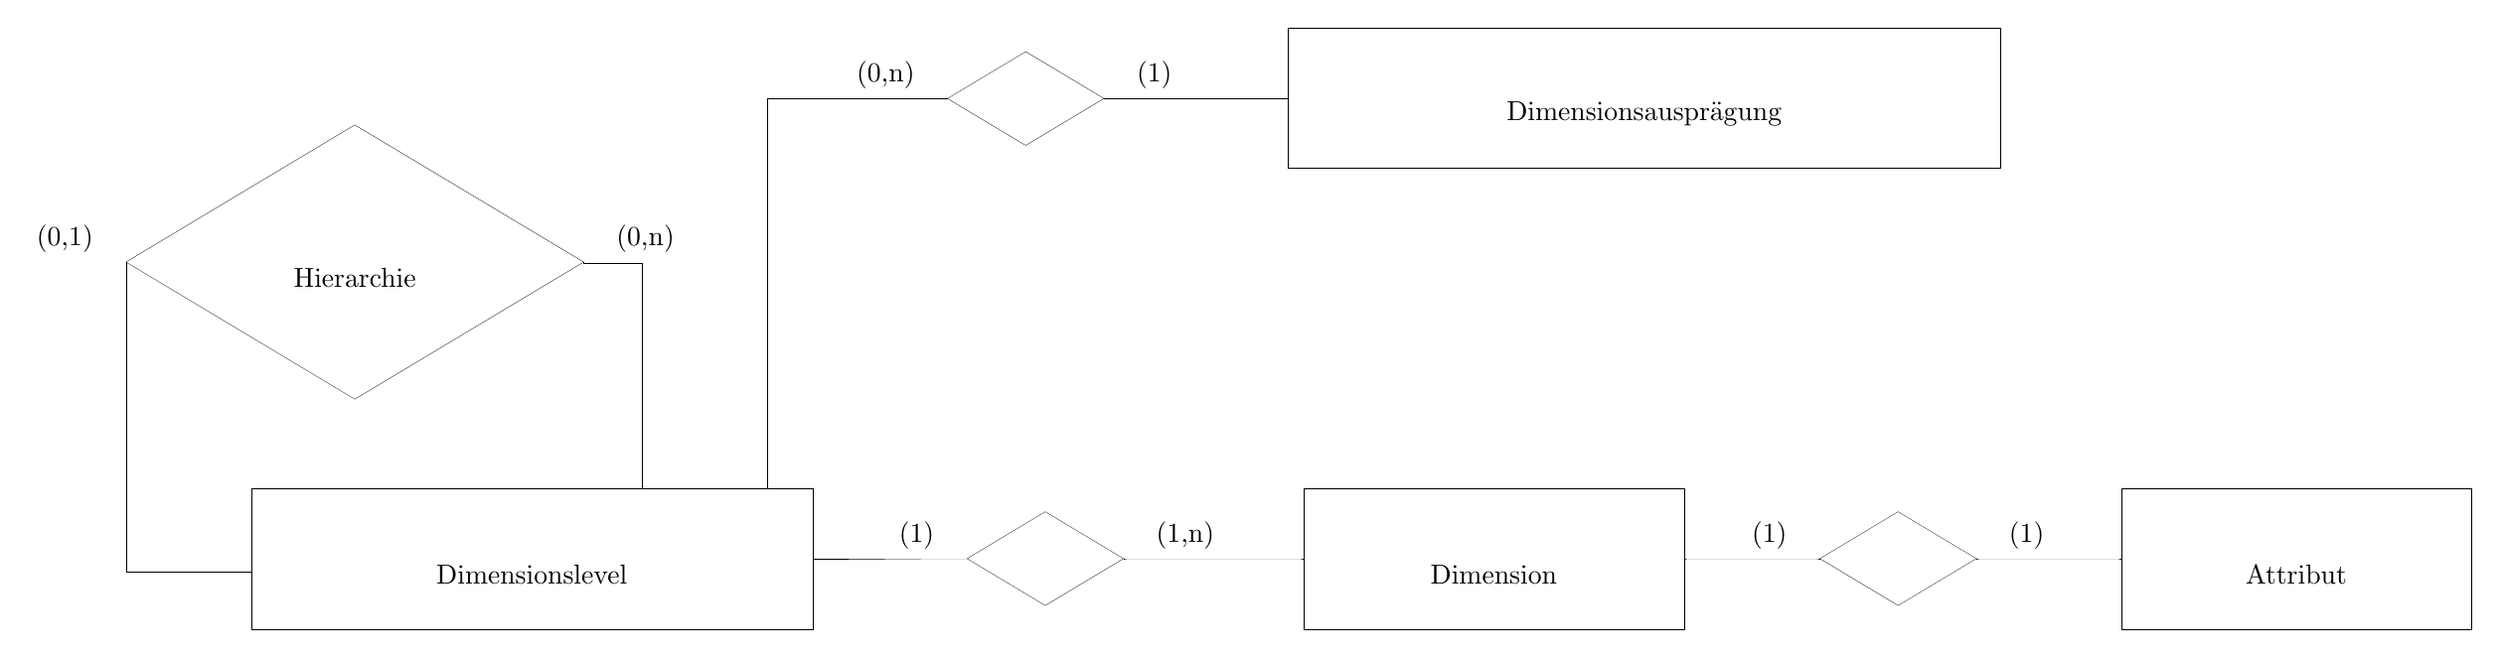
\begin{tikzpicture}
\pgftransformxscale{1.000000}
\pgftransformyscale{-1.000000}
\definecolor{dialinecolor}{rgb}{0.000000, 0.000000, 0.000000}
\pgfsetstrokecolor{dialinecolor}
\definecolor{dialinecolor}{rgb}{1.000000, 1.000000, 1.000000}
\pgfsetfillcolor{dialinecolor}
\definecolor{dialinecolor}{rgb}{1.000000, 1.000000, 1.000000}
\pgfsetfillcolor{dialinecolor}
\fill (26.650000\du,14.200000\du)--(26.650000\du,16.000000\du)--(31.515000\du,16.000000\du)--(31.515000\du,14.200000\du)--cycle;
\pgfsetlinewidth{0.100000\du}
\pgfsetdash{}{0pt}
\pgfsetmiterjoin
\definecolor{dialinecolor}{rgb}{0.000000, 0.000000, 0.000000}
\pgfsetstrokecolor{dialinecolor}
\draw (26.650000\du,14.200000\du)--(26.650000\du,16.000000\du)--(31.515000\du,16.000000\du)--(31.515000\du,14.200000\du)--cycle;
% setfont left to latex
\definecolor{dialinecolor}{rgb}{0.000000, 0.000000, 0.000000}
\pgfsetstrokecolor{dialinecolor}
\node at (29.082500\du,15.300000\du){Dimension};
\definecolor{dialinecolor}{rgb}{1.000000, 1.000000, 1.000000}
\pgfsetfillcolor{dialinecolor}
\fill (13.200000\du,14.200000\du)--(13.200000\du,16.000000\du)--(20.375000\du,16.000000\du)--(20.375000\du,14.200000\du)--cycle;
\pgfsetlinewidth{0.100000\du}
\pgfsetdash{}{0pt}
\pgfsetmiterjoin
\definecolor{dialinecolor}{rgb}{0.000000, 0.000000, 0.000000}
\pgfsetstrokecolor{dialinecolor}
\draw (13.200000\du,14.200000\du)--(13.200000\du,16.000000\du)--(20.375000\du,16.000000\du)--(20.375000\du,14.200000\du)--cycle;
% setfont left to latex
\definecolor{dialinecolor}{rgb}{0.000000, 0.000000, 0.000000}
\pgfsetstrokecolor{dialinecolor}
\node at (16.787500\du,15.300000\du){Dimensionslevel};
\definecolor{dialinecolor}{rgb}{1.000000, 1.000000, 1.000000}
\pgfsetfillcolor{dialinecolor}
\fill (37.100000\du,14.200000\du)--(37.100000\du,16.000000\du)--(41.580000\du,16.000000\du)--(41.580000\du,14.200000\du)--cycle;
\pgfsetlinewidth{0.100000\du}
\pgfsetdash{}{0pt}
\pgfsetmiterjoin
\definecolor{dialinecolor}{rgb}{0.000000, 0.000000, 0.000000}
\pgfsetstrokecolor{dialinecolor}
\draw (37.100000\du,14.200000\du)--(37.100000\du,16.000000\du)--(41.580000\du,16.000000\du)--(41.580000\du,14.200000\du)--cycle;
% setfont left to latex
\definecolor{dialinecolor}{rgb}{0.000000, 0.000000, 0.000000}
\pgfsetstrokecolor{dialinecolor}
\node at (39.340000\du,15.300000\du){Attribut};
\definecolor{dialinecolor}{rgb}{1.000000, 1.000000, 1.000000}
\pgfsetfillcolor{dialinecolor}
\fill (11.600000\du,11.305000\du)--(14.525000\du,9.550000\du)--(17.450000\du,11.305000\du)--(14.525000\du,13.060000\du)--cycle;
\pgfsetlinewidth{0.100000\du}
\pgfsetdash{}{0pt}
\pgfsetmiterjoin
\definecolor{dialinecolor}{rgb}{0.000000, 0.000000, 0.000000}
\pgfsetstrokecolor{dialinecolor}
\draw (11.600000\du,11.305000\du)--(14.525000\du,9.550000\du)--(17.450000\du,11.305000\du)--(14.525000\du,13.060000\du)--cycle;
% setfont left to latex
\definecolor{dialinecolor}{rgb}{0.000000, 0.000000, 0.000000}
\pgfsetstrokecolor{dialinecolor}
\node[anchor=east] at (11.300000\du,11.005000\du){(0,1)};
\definecolor{dialinecolor}{rgb}{0.000000, 0.000000, 0.000000}
\pgfsetstrokecolor{dialinecolor}
\node[anchor=west] at (17.750000\du,11.005000\du){(0,n)};
\definecolor{dialinecolor}{rgb}{0.000000, 0.000000, 0.000000}
\pgfsetstrokecolor{dialinecolor}
\node at (14.525000\du,11.505000\du){Hierarchie};
\pgfsetlinewidth{0.100000\du}
\pgfsetdash{}{0pt}
\pgfsetmiterjoin
\pgfsetbuttcap
\definecolor{dialinecolor}{rgb}{0.000000, 0.000000, 0.000000}
\pgfsetstrokecolor{dialinecolor}
\draw (13.200000\du,15.100000\du)--(13.200000\du,15.269600\du)--(11.600000\du,15.269600\du)--(11.600000\du,11.305000\du);
\pgfsetlinewidth{0.100000\du}
\pgfsetdash{}{0pt}
\pgfsetmiterjoin
\pgfsetbuttcap
\definecolor{dialinecolor}{rgb}{0.000000, 0.000000, 0.000000}
\pgfsetstrokecolor{dialinecolor}
\draw (16.787500\du,14.200000\du)--(18.200000\du,14.200000\du)--(18.200000\du,11.319600\du)--(17.450000\du,11.319600\du)--(17.450000\du,11.305000\du);
\definecolor{dialinecolor}{rgb}{1.000000, 1.000000, 1.000000}
\pgfsetfillcolor{dialinecolor}
\fill (22.350000\du,15.100000\du)--(23.350000\du,14.500000\du)--(24.350000\du,15.100000\du)--(23.350000\du,15.700000\du)--cycle;
\pgfsetlinewidth{0.100000\du}
\pgfsetdash{}{0pt}
\pgfsetmiterjoin
\definecolor{dialinecolor}{rgb}{0.000000, 0.000000, 0.000000}
\pgfsetstrokecolor{dialinecolor}
\draw (22.350000\du,15.100000\du)--(23.350000\du,14.500000\du)--(24.350000\du,15.100000\du)--(23.350000\du,15.700000\du)--cycle;
% setfont left to latex
\definecolor{dialinecolor}{rgb}{0.000000, 0.000000, 0.000000}
\pgfsetstrokecolor{dialinecolor}
\node[anchor=east] at (22.050000\du,14.800000\du){(1) };
\definecolor{dialinecolor}{rgb}{0.000000, 0.000000, 0.000000}
\pgfsetstrokecolor{dialinecolor}
\node[anchor=west] at (24.650000\du,14.800000\du){(1,n) };
\definecolor{dialinecolor}{rgb}{0.000000, 0.000000, 0.000000}
\pgfsetstrokecolor{dialinecolor}
\node at (23.350000\du,15.300000\du){};
\pgfsetlinewidth{0.100000\du}
\pgfsetdash{}{0pt}
\pgfsetmiterjoin
\pgfsetbuttcap
\definecolor{dialinecolor}{rgb}{0.000000, 0.000000, 0.000000}
\pgfsetstrokecolor{dialinecolor}
\draw (26.650000\du,15.100000\du)--(26.600000\du,15.100000\du)--(24.400000\du,15.100000\du)--(24.350000\du,15.100000\du);
\pgfsetlinewidth{0.100000\du}
\pgfsetdash{}{0pt}
\pgfsetmiterjoin
\pgfsetbuttcap
\definecolor{dialinecolor}{rgb}{0.000000, 0.000000, 0.000000}
\pgfsetstrokecolor{dialinecolor}
\draw (22.350000\du,15.100000\du)--(22.200000\du,15.100000\du)--(22.200000\du,15.100000\du)--(20.375000\du,15.100000\du);
\definecolor{dialinecolor}{rgb}{1.000000, 1.000000, 1.000000}
\pgfsetfillcolor{dialinecolor}
\fill (33.250000\du,15.100000\du)--(34.250000\du,14.500000\du)--(35.250000\du,15.100000\du)--(34.250000\du,15.700000\du)--cycle;
\pgfsetlinewidth{0.100000\du}
\pgfsetdash{}{0pt}
\pgfsetmiterjoin
\definecolor{dialinecolor}{rgb}{0.000000, 0.000000, 0.000000}
\pgfsetstrokecolor{dialinecolor}
\draw (33.250000\du,15.100000\du)--(34.250000\du,14.500000\du)--(35.250000\du,15.100000\du)--(34.250000\du,15.700000\du)--cycle;
% setfont left to latex
\definecolor{dialinecolor}{rgb}{0.000000, 0.000000, 0.000000}
\pgfsetstrokecolor{dialinecolor}
\node[anchor=east] at (32.950000\du,14.800000\du){(1)};
\definecolor{dialinecolor}{rgb}{0.000000, 0.000000, 0.000000}
\pgfsetstrokecolor{dialinecolor}
\node[anchor=west] at (35.550000\du,14.800000\du){(1)};
\definecolor{dialinecolor}{rgb}{0.000000, 0.000000, 0.000000}
\pgfsetstrokecolor{dialinecolor}
\node at (34.250000\du,15.300000\du){};
\definecolor{dialinecolor}{rgb}{1.000000, 1.000000, 1.000000}
\pgfsetfillcolor{dialinecolor}
\fill (22.100000\du,9.212500\du)--(23.100000\du,8.612500\du)--(24.100000\du,9.212500\du)--(23.100000\du,9.812500\du)--cycle;
\pgfsetlinewidth{0.100000\du}
\pgfsetdash{}{0pt}
\pgfsetmiterjoin
\definecolor{dialinecolor}{rgb}{0.000000, 0.000000, 0.000000}
\pgfsetstrokecolor{dialinecolor}
\draw (22.100000\du,9.212500\du)--(23.100000\du,8.612500\du)--(24.100000\du,9.212500\du)--(23.100000\du,9.812500\du)--cycle;
% setfont left to latex
\definecolor{dialinecolor}{rgb}{0.000000, 0.000000, 0.000000}
\pgfsetstrokecolor{dialinecolor}
\node[anchor=east] at (21.800000\du,8.912500\du){(0,n)};
\definecolor{dialinecolor}{rgb}{0.000000, 0.000000, 0.000000}
\pgfsetstrokecolor{dialinecolor}
\node[anchor=west] at (24.400000\du,8.912500\du){(1)};
\definecolor{dialinecolor}{rgb}{0.000000, 0.000000, 0.000000}
\pgfsetstrokecolor{dialinecolor}
\node at (23.100000\du,9.412500\du){};
\pgfsetlinewidth{0.100000\du}
\pgfsetdash{}{0pt}
\pgfsetmiterjoin
\pgfsetbuttcap
\definecolor{dialinecolor}{rgb}{0.000000, 0.000000, 0.000000}
\pgfsetstrokecolor{dialinecolor}
\draw (33.250000\du,15.100000\du)--(33.200000\du,15.100000\du)--(31.565000\du,15.100000\du)--(31.515000\du,15.100000\du);
\pgfsetlinewidth{0.100000\du}
\pgfsetdash{}{0pt}
\pgfsetmiterjoin
\pgfsetbuttcap
\definecolor{dialinecolor}{rgb}{0.000000, 0.000000, 0.000000}
\pgfsetstrokecolor{dialinecolor}
\draw (35.250000\du,15.100000\du)--(35.300000\du,15.100000\du)--(37.050000\du,15.100000\du)--(37.100000\du,15.100000\du);
\pgfsetlinewidth{0.100000\du}
\pgfsetdash{}{0pt}
\pgfsetmiterjoin
\pgfsetbuttcap
\definecolor{dialinecolor}{rgb}{0.000000, 0.000000, 0.000000}
\pgfsetstrokecolor{dialinecolor}
\draw (20.375000\du,14.200000\du)--(19.800000\du,14.200000\du)--(19.800000\du,9.212500\du)--(22.100000\du,9.212500\du);
\pgfsetlinewidth{0.100000\du}
\pgfsetdash{}{0pt}
\pgfsetmiterjoin
\pgfsetbuttcap
\definecolor{dialinecolor}{rgb}{0.000000, 0.000000, 0.000000}
\pgfsetstrokecolor{dialinecolor}
\draw (24.100000\du,9.212500\du)--(25.277500\du,9.212500\du)--(25.277500\du,9.205000\du)--(26.455000\du,9.205000\du);
\definecolor{dialinecolor}{rgb}{1.000000, 1.000000, 1.000000}
\pgfsetfillcolor{dialinecolor}
\fill (26.455000\du,8.305000\du)--(26.455000\du,10.105000\du)--(35.555000\du,10.105000\du)--(35.555000\du,8.305000\du)--cycle;
\pgfsetlinewidth{0.100000\du}
\pgfsetdash{}{0pt}
\pgfsetmiterjoin
\definecolor{dialinecolor}{rgb}{0.000000, 0.000000, 0.000000}
\pgfsetstrokecolor{dialinecolor}
\draw (26.455000\du,8.305000\du)--(26.455000\du,10.105000\du)--(35.555000\du,10.105000\du)--(35.555000\du,8.305000\du)--cycle;
% setfont left to latex
\definecolor{dialinecolor}{rgb}{0.000000, 0.000000, 0.000000}
\pgfsetstrokecolor{dialinecolor}
\node at (31.005000\du,9.405000\du){Dimensionsausprägung};
\end{tikzpicture}
}
    \caption{\acrshort{ERM} der Dimensionteilsprache}\label{dimension-erm}
  \end{figure}

	Eine Dimension wird hierarchisch unterteilt in Dimensionslevel, welche die
	Informationen einer Attributinstanz in Teilinformationen einteilen. Die Tiefe
	einer Dimensionslevelhierarchie ist beliebig. Das Attribut
	\textit{Verfallsdatum} kann zum Beispiel die Instanz '09.08.2016' haben. Wird
	hierauf die Dimension \textit{Zeit} angewendet, kann die Instanz in den
	Dimensionsleveln \textit{Jahr} '2016', \textit{Monat} '08' und \textit{Tag}
	'09' unterschieden werden. Das Dimensionslevel \textit{Monat} ist hier dem
	Dimensionslevel \textit{Jahr} hierarchisch untergeordnet. Die
	Teilinformationen bilden die Dimensionslevelausprägungen. Im oben genannten
	Beispiel ist '2016' eine Dimensionslevelausprägung des Dimensionslevels
	\textit{Jahr} der Dimension \textit{Zeit} des Attributs
	\textit{Verfallsdatum}. In Abbildung~\ref{dimension-erm} wird dieses
	Konstrukt mit Hilfe eines \acrshort{ERM}s verdeutlicht.

  \subsection{Kennzahlen}
  \todo[inline]{Konstanten in Grafik, \textit{DataFurnace} und Text hinzufügen}

  \begin{figure}
    \resizebox{250px}{!}{% Graphic for TeX using PGF
% Title: /home/indenml/code/bachelor_thesis/content/figures/language_spec-erm-geschaeftsobjekt.dia
% Creator: Dia v0.97.3
% CreationDate: Tue Sep 27 11:17:50 2016
% For: indenml
% \usepackage{tikz}
% The following commands are not supported in PSTricks at present
% We define them conditionally, so when they are implemented,
% this pgf file will use them.
\ifx\du\undefined
  \newlength{\du}
\fi
\setlength{\du}{15\unitlength}
\begin{tikzpicture}
\pgftransformxscale{1.171906}
\pgftransformyscale{-1.171906}
\definecolor{dialinecolor}{rgb}{0.000000, 0.000000, 0.000000}
\pgfsetstrokecolor{dialinecolor}
\definecolor{dialinecolor}{rgb}{1.000000, 1.000000, 1.000000}
\pgfsetfillcolor{dialinecolor}
\definecolor{dialinecolor}{rgb}{1.000000, 1.000000, 1.000000}
\pgfsetfillcolor{dialinecolor}
\fill (14.242400\du,25.644600\du)--(14.242400\du,27.444600\du)--(18.722400\du,27.444600\du)--(18.722400\du,25.644600\du)--cycle;
\pgfsetlinewidth{0.100000\du}
\pgfsetdash{}{0pt}
\pgfsetmiterjoin
\definecolor{dialinecolor}{rgb}{0.000000, 0.000000, 0.000000}
\pgfsetstrokecolor{dialinecolor}
\draw (14.242400\du,25.644600\du)--(14.242400\du,27.444600\du)--(18.722400\du,27.444600\du)--(18.722400\du,25.644600\du)--cycle;
% setfont left to latex
\definecolor{dialinecolor}{rgb}{0.000000, 0.000000, 0.000000}
\pgfsetstrokecolor{dialinecolor}
\node at (16.482400\du,26.744600\du){Kennzahl};
\definecolor{dialinecolor}{rgb}{1.000000, 1.000000, 1.000000}
\pgfsetfillcolor{dialinecolor}
\fill (14.244400\du,33.701100\du)--(14.244400\du,35.501100\du)--(18.724400\du,35.501100\du)--(18.724400\du,33.701100\du)--cycle;
\pgfsetlinewidth{0.100000\du}
\pgfsetdash{}{0pt}
\pgfsetmiterjoin
\definecolor{dialinecolor}{rgb}{0.000000, 0.000000, 0.000000}
\pgfsetstrokecolor{dialinecolor}
\draw (14.244400\du,33.701100\du)--(14.244400\du,35.501100\du)--(18.724400\du,35.501100\du)--(18.724400\du,33.701100\du)--cycle;
% setfont left to latex
\definecolor{dialinecolor}{rgb}{0.000000, 0.000000, 0.000000}
\pgfsetstrokecolor{dialinecolor}
\node at (16.484400\du,34.801100\du){Ausdruck};
\definecolor{dialinecolor}{rgb}{1.000000, 1.000000, 1.000000}
\pgfsetfillcolor{dialinecolor}
\fill (14.329000\du,30.760100\du)--(16.484000\du,29.467100\du)--(18.639000\du,30.760100\du)--(16.484000\du,32.053100\du)--cycle;
\pgfsetlinewidth{0.100000\du}
\pgfsetdash{}{0pt}
\pgfsetmiterjoin
\definecolor{dialinecolor}{rgb}{0.000000, 0.000000, 0.000000}
\pgfsetstrokecolor{dialinecolor}
\draw (14.329000\du,30.760100\du)--(16.484000\du,29.467100\du)--(18.639000\du,30.760100\du)--(16.484000\du,32.053100\du)--cycle;
% setfont left to latex
\definecolor{dialinecolor}{rgb}{0.000000, 0.000000, 0.000000}
\pgfsetstrokecolor{dialinecolor}
\node[anchor=west] at (16.684000\du,29.167100\du){(1,n)};
\definecolor{dialinecolor}{rgb}{0.000000, 0.000000, 0.000000}
\pgfsetstrokecolor{dialinecolor}
\node[anchor=west] at (16.684000\du,33.153100\du){(1)};
\definecolor{dialinecolor}{rgb}{0.000000, 0.000000, 0.000000}
\pgfsetstrokecolor{dialinecolor}
\node at (16.484000\du,30.960100\du){Formel};
\pgfsetlinewidth{0.100000\du}
\pgfsetdash{}{0pt}
\pgfsetmiterjoin
\pgfsetbuttcap
\definecolor{dialinecolor}{rgb}{0.000000, 0.000000, 0.000000}
\pgfsetstrokecolor{dialinecolor}
\draw (16.482400\du,27.444600\du)--(16.482400\du,27.437200\du)--(16.484000\du,27.437200\du)--(16.484000\du,29.467100\du);
\pgfsetlinewidth{0.100000\du}
\pgfsetdash{}{0pt}
\pgfsetmiterjoin
\pgfsetbuttcap
\definecolor{dialinecolor}{rgb}{0.000000, 0.000000, 0.000000}
\pgfsetstrokecolor{dialinecolor}
\draw (16.484000\du,32.053100\du)--(16.483900\du,32.053100\du)--(16.483900\du,33.701100\du)--(16.484400\du,33.701100\du);
\pgfsetlinewidth{0.100000\du}
\pgfsetdash{}{0pt}
\pgfsetdash{}{0pt}
\pgfsetbuttcap
\pgfsetmiterjoin
\pgfsetlinewidth{0.100000\du}
\pgfsetbuttcap
\pgfsetmiterjoin
\pgfsetdash{}{0pt}
\definecolor{dialinecolor}{rgb}{1.000000, 1.000000, 1.000000}
\pgfsetfillcolor{dialinecolor}
\fill (15.059400\du,39.100028\du)--(17.829400\du,39.100028\du)--(16.444400\du,36.900028\du)--cycle;
\definecolor{dialinecolor}{rgb}{0.000000, 0.000000, 0.000000}
\pgfsetstrokecolor{dialinecolor}
\draw (15.059400\du,39.100028\du)--(17.829400\du,39.100028\du)--(16.444400\du,36.900028\du)--cycle;
% setfont left to latex
\definecolor{dialinecolor}{rgb}{0.000000, 0.000000, 0.000000}
\pgfsetstrokecolor{dialinecolor}
\node at (16.444400\du,38.750028\du){D,T};
\definecolor{dialinecolor}{rgb}{1.000000, 1.000000, 1.000000}
\pgfsetfillcolor{dialinecolor}
\fill (26.404400\du,41.356500\du)--(26.404400\du,43.156500\du)--(30.884400\du,43.156500\du)--(30.884400\du,41.356500\du)--cycle;
\pgfsetlinewidth{0.100000\du}
\pgfsetdash{}{0pt}
\pgfsetmiterjoin
\definecolor{dialinecolor}{rgb}{0.000000, 0.000000, 0.000000}
\pgfsetstrokecolor{dialinecolor}
\draw (26.404400\du,41.356500\du)--(26.404400\du,43.156500\du)--(30.884400\du,43.156500\du)--(30.884400\du,41.356500\du)--cycle;
% setfont left to latex
\definecolor{dialinecolor}{rgb}{0.000000, 0.000000, 0.000000}
\pgfsetstrokecolor{dialinecolor}
\node at (28.644400\du,42.456500\du){Funktion};
\definecolor{dialinecolor}{rgb}{1.000000, 1.000000, 1.000000}
\pgfsetfillcolor{dialinecolor}
\fill (12.104400\du,41.306500\du)--(12.104400\du,43.106500\du)--(16.584400\du,43.106500\du)--(16.584400\du,41.306500\du)--cycle;
\pgfsetlinewidth{0.100000\du}
\pgfsetdash{}{0pt}
\pgfsetmiterjoin
\definecolor{dialinecolor}{rgb}{0.000000, 0.000000, 0.000000}
\pgfsetstrokecolor{dialinecolor}
\draw (12.104400\du,41.306500\du)--(12.104400\du,43.106500\du)--(16.584400\du,43.106500\du)--(16.584400\du,41.306500\du)--cycle;
% setfont left to latex
\definecolor{dialinecolor}{rgb}{0.000000, 0.000000, 0.000000}
\pgfsetstrokecolor{dialinecolor}
\node at (14.344400\du,42.406500\du){Operator};
\definecolor{dialinecolor}{rgb}{1.000000, 1.000000, 1.000000}
\pgfsetfillcolor{dialinecolor}
\fill (19.854400\du,41.456500\du)--(19.854400\du,43.256500\du)--(23.949400\du,43.256500\du)--(23.949400\du,41.456500\du)--cycle;
\pgfsetlinewidth{0.100000\du}
\pgfsetdash{}{0pt}
\pgfsetmiterjoin
\definecolor{dialinecolor}{rgb}{0.000000, 0.000000, 0.000000}
\pgfsetstrokecolor{dialinecolor}
\draw (19.854400\du,41.456500\du)--(19.854400\du,43.256500\du)--(23.949400\du,43.256500\du)--(23.949400\du,41.456500\du)--cycle;
% setfont left to latex
\definecolor{dialinecolor}{rgb}{0.000000, 0.000000, 0.000000}
\pgfsetstrokecolor{dialinecolor}
\node at (21.901900\du,42.556500\du){Klammer};
\definecolor{dialinecolor}{rgb}{1.000000, 1.000000, 1.000000}
\pgfsetfillcolor{dialinecolor}
\fill (6.744370\du,44.251500\du)--(6.744370\du,46.051500\du)--(13.919370\du,46.051500\du)--(13.919370\du,44.251500\du)--cycle;
\pgfsetlinewidth{0.100000\du}
\pgfsetdash{}{0pt}
\pgfsetmiterjoin
\definecolor{dialinecolor}{rgb}{0.000000, 0.000000, 0.000000}
\pgfsetstrokecolor{dialinecolor}
\draw (6.744370\du,44.251500\du)--(6.744370\du,46.051500\du)--(13.919370\du,46.051500\du)--(13.919370\du,44.251500\du)--cycle;
% setfont left to latex
\definecolor{dialinecolor}{rgb}{0.000000, 0.000000, 0.000000}
\pgfsetstrokecolor{dialinecolor}
\node at (10.331870\du,45.351500\du){Kennzahlverweis};
\definecolor{dialinecolor}{rgb}{1.000000, 1.000000, 1.000000}
\pgfsetfillcolor{dialinecolor}
\fill (14.634400\du,44.271500\du)--(14.634400\du,46.071500\du)--(21.809400\du,46.071500\du)--(21.809400\du,44.271500\du)--cycle;
\pgfsetlinewidth{0.100000\du}
\pgfsetdash{}{0pt}
\pgfsetmiterjoin
\definecolor{dialinecolor}{rgb}{0.000000, 0.000000, 0.000000}
\pgfsetstrokecolor{dialinecolor}
\draw (14.634400\du,44.271500\du)--(14.634400\du,46.071500\du)--(21.809400\du,46.071500\du)--(21.809400\du,44.271500\du)--cycle;
% setfont left to latex
\definecolor{dialinecolor}{rgb}{0.000000, 0.000000, 0.000000}
\pgfsetstrokecolor{dialinecolor}
\node at (18.221900\du,45.371500\du){Attributverweis};
\definecolor{dialinecolor}{rgb}{1.000000, 1.000000, 1.000000}
\pgfsetfillcolor{dialinecolor}
\fill (22.404400\du,44.241500\du)--(22.404400\du,46.041500\du)--(27.269400\du,46.041500\du)--(27.269400\du,44.241500\du)--cycle;
\pgfsetlinewidth{0.100000\du}
\pgfsetdash{}{0pt}
\pgfsetmiterjoin
\definecolor{dialinecolor}{rgb}{0.000000, 0.000000, 0.000000}
\pgfsetstrokecolor{dialinecolor}
\draw (22.404400\du,44.241500\du)--(22.404400\du,46.041500\du)--(27.269400\du,46.041500\du)--(27.269400\du,44.241500\du)--cycle;
% setfont left to latex
\definecolor{dialinecolor}{rgb}{0.000000, 0.000000, 0.000000}
\pgfsetstrokecolor{dialinecolor}
\node at (24.836900\du,45.341500\du){Konstante};
\pgfsetlinewidth{0.100000\du}
\pgfsetdash{}{0pt}
\pgfsetmiterjoin
\pgfsetbuttcap
\definecolor{dialinecolor}{rgb}{0.000000, 0.000000, 0.000000}
\pgfsetstrokecolor{dialinecolor}
\draw (28.644400\du,41.356500\du)--(28.644400\du,40.500000\du)--(16.444400\du,40.500000\du)--(16.444400\du,39.100028\du);
\pgfsetlinewidth{0.100000\du}
\pgfsetdash{}{0pt}
\pgfsetmiterjoin
\pgfsetbuttcap
\definecolor{dialinecolor}{rgb}{0.000000, 0.000000, 0.000000}
\pgfsetstrokecolor{dialinecolor}
\draw (14.344400\du,41.306500\du)--(14.344400\du,40.506300\du)--(16.444400\du,40.506300\du)--(16.444400\du,39.100028\du);
\pgfsetlinewidth{0.100000\du}
\pgfsetdash{}{0pt}
\pgfsetmiterjoin
\pgfsetbuttcap
\definecolor{dialinecolor}{rgb}{0.000000, 0.000000, 0.000000}
\pgfsetstrokecolor{dialinecolor}
\draw (10.331870\du,44.251500\du)--(10.331870\du,40.512500\du)--(16.444400\du,40.512500\du)--(16.444400\du,39.100028\du);
\pgfsetlinewidth{0.100000\du}
\pgfsetdash{}{0pt}
\pgfsetmiterjoin
\pgfsetbuttcap
\definecolor{dialinecolor}{rgb}{0.000000, 0.000000, 0.000000}
\pgfsetstrokecolor{dialinecolor}
\draw (18.221900\du,44.271500\du)--(18.221900\du,40.512500\du)--(16.444400\du,40.512500\du)--(16.444400\du,39.100028\du);
\pgfsetlinewidth{0.100000\du}
\pgfsetdash{}{0pt}
\pgfsetmiterjoin
\pgfsetbuttcap
\definecolor{dialinecolor}{rgb}{0.000000, 0.000000, 0.000000}
\pgfsetstrokecolor{dialinecolor}
\draw (21.901900\du,41.456500\du)--(21.901900\du,40.501500\du)--(16.444400\du,40.501500\du)--(16.444400\du,39.100028\du);
\pgfsetlinewidth{0.100000\du}
\pgfsetdash{}{0pt}
\pgfsetmiterjoin
\pgfsetbuttcap
\definecolor{dialinecolor}{rgb}{0.000000, 0.000000, 0.000000}
\pgfsetstrokecolor{dialinecolor}
\draw (24.836900\du,44.241500\du)--(24.836900\du,40.512500\du)--(16.444400\du,40.512500\du)--(16.444400\du,39.100028\du);
\pgfsetlinewidth{0.100000\du}
\pgfsetdash{}{0pt}
\pgfsetmiterjoin
\pgfsetbuttcap
\definecolor{dialinecolor}{rgb}{0.000000, 0.000000, 0.000000}
\pgfsetstrokecolor{dialinecolor}
\draw (16.444400\du,36.900028\du)--(16.444400\du,36.212500\du)--(16.484400\du,36.212500\du)--(16.484400\du,35.501100\du);
\end{tikzpicture}
}
    \caption{\acrshort{ERM} der Kennzahlteilsprache}\label{kennzahl}
  \end{figure}

	Eine Kennzahl bietet ein quantitatives Maß, welches die Informationen von
	einer Instanz eines Geschäftsobjekts weiterverarbeitet. Sie
	wird durch eine mathematische Formel spezifiziert, und folgt der
	Grundrechenart mit den Operationen \textit{Addition}, \textit{Substraktion},
	\textit{Multiplikation} und \textit{Division}, welche auf zwei oder mehr
	Operanden angewendet werden (Siehe Abbildung~\ref{railroad-kennzahl}, Gleis
	eins). Im weiteren Verlauf der \textit{DataFurnace}-Sprachvorstellung wird
	der Begriff \textit{Ausdruck} als Generalisierung von \textit{Operand} und
	\textit{Operator} genutzt.  Die Auswertungsreihenfolge der Ausdrücke kann mit
	Klammern differenziert werden, erneut verdeutlicht durch
	Abbildung~\ref{railroad-kennzahl}, Gleis zwei.  Ausdrücke können mit dem
	Voranstellen eines Minuszeichens negiert werden (Siehe
	Abbildung~\ref{railroad-kennzahl}, Gleis drei). Des Weiteren können
	Konstanten in die Formelgleichung mit aufgenommen werden.

  % Diagram(
  %   Choice(1,
  %     Sequence('Ausdruck', Choice(1, '+', '-', '*', '/'), 'Ausdruck'),
  %     Sequence('(', 'Ausdruck', ')'),
  %     Sequence('-', 'Ausdruck'),
  %     'Attribut',
  %     Sequence('Funktion', '(', 'Ausdruck', ')'),
  %     'Kennzahl'
  %   )
  % )

  \todo[inline]{Verweise auf die Gleis-Nummern im Text überprüfen}
  \begin{figure}
    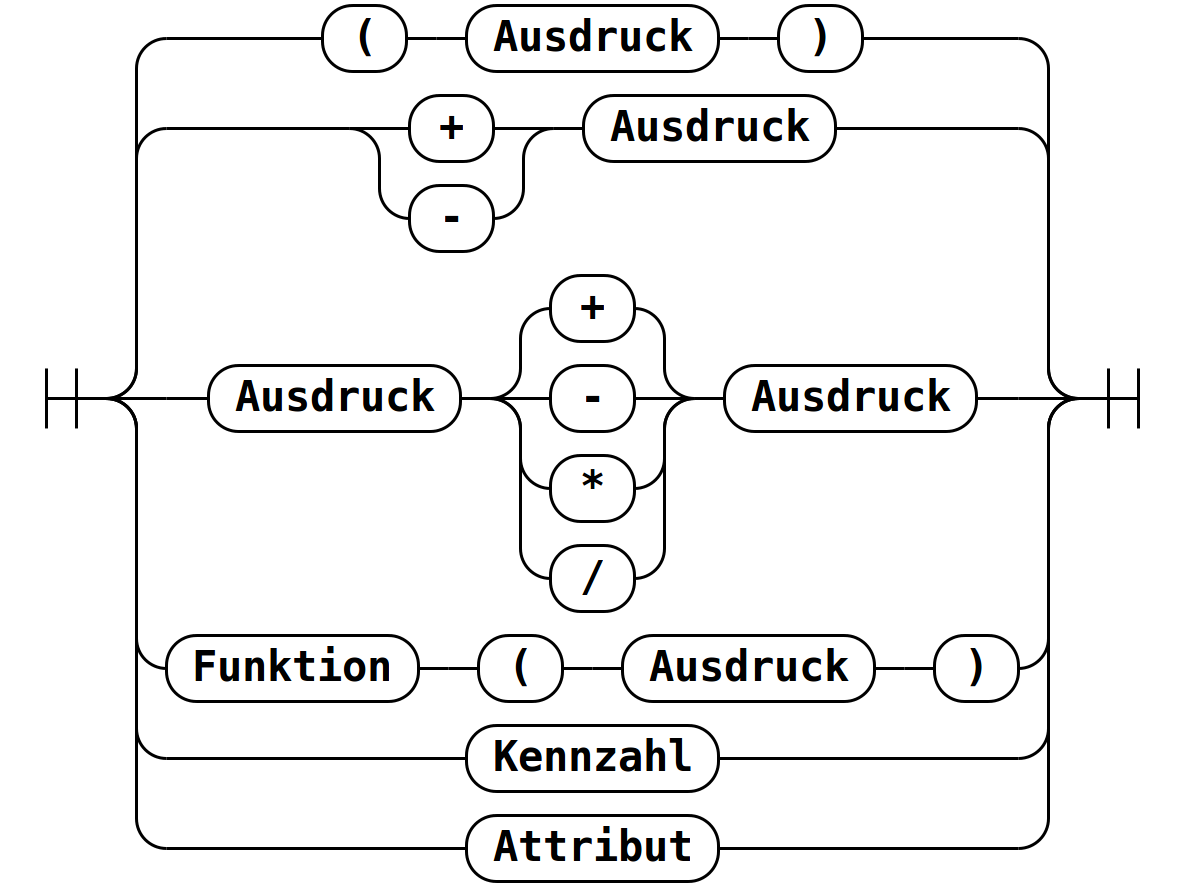
\includegraphics[scale=0.25]{content/figures/railroad-kennzahl.png}
    \caption[Ausdruck Syntaxdiagramm]{Ausdruck Syntaxdiagramm \protect\footnotemark}\label{railroad-kennzahl}
  \end{figure}
  \footnotetext{\texthl{Informatik, Beschreibung von Programmiersprachen,
  Compiler, Railroad-Diagram, horizontale Linien gleich Gleise, Stationen erklaeren}}
	
  Um innerhalb der Formel einer Kennzahl auf die Informationen einer
  Geschäftsobjektinstanz zugreifen zu können, können die Attribute des
  Geschäftsobjekts als Formelausdruck eingebracht werden, wie in
  Abbildung~\ref{railroad-kennzahl} durch die Station \textit{Attribut}
  verdeutlicht. Hierzu wird innerhalb der Formel auf das konkrete Attribut
  eines bestimmten Geschäftsobjekts, und nicht, wie in der Sprache \textit{H2
  for Reporting}, auf ein variables Attribut ohne Referenz zu einem
  Bezugsobjekt, verwiesen~\cite[][S.  20]{becker2007h2}. Dieses Vorgehen
  verhindert die generische Definition und Wiederverwendbarkeit von Kennzahlen,
  ermöglicht jedoch eine situationsnahe Konzeption und einen geringeren
  Konfigurationsaufwand im späteren Gebrauch der Kennzahl.

  Neben den mathematischen Grundlagen sollen weitere Verarbeitungsmöglichkeiten
  bereitgestellt werden. Hierzu dient die Ausdruckskategorie \textit{Funktion}
  (Siehe Abbildung~\ref{railroad-kennzahl} Gleis fünf). Eine Funktion nimmt als
  Eingabe einen oder mehrere Ausdrücke und gibt im Gegenzug einen solchen
  zurück. Sie abstrahiert bei diesem Vorgang von der eigentlichen Umsetzung im
  Inneren, und ermöglicht den Fokus auf das Ergebnis selbst. Eine Funktion kann
  sich immer nur auf Attribute einer Geschäftsobjektinstanz beziehen. Die
  Aggregation von mehreren Geschäftsobjektinstanzen findet in den
  Berichtsteilsprache statt, nicht in der Kennzahlteilsprache.

	Ein Beispiel für eine Funktion ist die \texttt{Wurzel}-Funktion.  Sie nimmt
	als Eingabe eine Zahl und gibt die Wurzel dieser zurück. Neben den
	mathematischen Funktionen wie der \texttt{Wurzel}-Funktion werden des
	Weiteren datenqualitätsspezifische Funktionen zur Verfügung gestellt, um
	Datensätze auf Datenqualitätsdimensionen zu lokalisieren, wie in
	Abschnitt~\ref{subsec:stammdatenqualität} vorgestellt.  Beispiele sind die
	\texttt{isEmpty}-Funktion, welche prüft ob ein Ausdruck Inhalt hat, und die
	\texttt{contains}-Funktion, welche zwei Ausdrücke als Parameter nimmt und
	kontrolliert ob der erste Audruck im zweiten Ausdruck vorhanden ist. Mit
	letzterer Funktion kann \zB{} geprüft werden, ob das Attribut
	\textit{E-Mail-Adresse} ein At-Zeichen enthält. Dies kann beispielsweise für
	eine Überprüfung der Datenqualitätsdimension \textit{einheitliche
	Darstellung} genutzt werden. Neben diesen beiden Qualitätskennzahlfunktionen
	kann der Nutzer außerdem Zeichenkettenlängen, Zahlen- und Datumsbereiche oder
	reguläre Ausdrücke für die Spezifikation von Qualitätskennzahlen nutzen.

  Um komplexe Ausdrücke strukturiert und abstrahiert beschreiben zu können,
  kann ein Ausdruck einer Kennzahl auch auf die Ergebnisse einer anderen
  Kennzahl zurückgreifen, verdeutlicht durch das letzte Gleis des
  Syntaxdiagramms (Abbildung~\ref{railroad-kennzahl}). Wird zum Beispiel die
  Kennzahl \textit{Gewinn} betrachtet, so kann diese aus der Subtraktion der
  Kennzahl \textit{Umsatz} als Minuend mit der Kennzahl \textit{Kosten} als
  Subtrahend berechnet werden.


  \subsection{Berichte}

  Das letzte Teilvokabular der \textit{DataFurnace}-Sprache ist der Bericht,
  welcher Dimensionen und Kenzahlen, wie in
  Abbildung~\ref{language_spec-erm-bericht} gezeigt, kombiniert. Ein Bericht
  bildet eine Fragestellung des Nutzers mit Bezug auf die Datenqualität seiner
  Geschäftsobjekte ab. Der Bericht wird unterteilt in eine Filterkomponente und
  eine Tabellenkomponente. Anhand dieser Zweiteilung wird im Folgenden die
  Teilsprache Bericht näher erläutert.

  \begin{figure}
    \resizebox{120px}{!}{% Graphic for TeX using PGF
% Title: /home/indenml/code/bachelor_thesis/content/figures/language_spec-erm.dia
% Creator: Dia v0.97.3
% CreationDate: Tue Sep 27 11:26:30 2016
% For: indenml
% \usepackage{tikz}
% The following commands are not supported in PSTricks at present
% We define them conditionally, so when they are implemented,
% this pgf file will use them.
\ifx\du\undefined{}
  \newlength{\du}
\fi
\setlength{\du}{15\unitlength}
\begin{tikzpicture}
\pgftransformxscale{1.000000}
\pgftransformyscale{-1.000000}
\definecolor{dialinecolor}{rgb}{0.000000, 0.000000, 0.000000}
\pgfsetstrokecolor{dialinecolor}
\definecolor{dialinecolor}{rgb}{1.000000, 1.000000, 1.000000}
\pgfsetfillcolor{dialinecolor}
\definecolor{dialinecolor}{rgb}{1.000000, 1.000000, 1.000000}
\pgfsetfillcolor{dialinecolor}
\fill (-3.210480\du,25.273700\du)--(-3.210480\du,27.073700\du)--(3.964520\du,27.073700\du)--(3.964520\du,25.273700\du)--cycle;
\pgfsetlinewidth{0.100000\du}
\pgfsetdash{}{0pt}
\pgfsetmiterjoin
\definecolor{dialinecolor}{rgb}{0.000000, 0.000000, 0.000000}
\pgfsetstrokecolor{dialinecolor}
\draw (-3.210480\du,25.273700\du)--(-3.210480\du,27.073700\du)--(3.964520\du,27.073700\du)--(3.964520\du,25.273700\du)--cycle;
% setfont left to latex
\definecolor{dialinecolor}{rgb}{0.000000, 0.000000, 0.000000}
\pgfsetstrokecolor{dialinecolor}
\node at (0.377020\du,26.373700\du){Dimensionslevel};
\definecolor{dialinecolor}{rgb}{1.000000, 1.000000, 1.000000}
\pgfsetfillcolor{dialinecolor}
\fill (14.242400\du,25.644600\du)--(14.242400\du,27.444600\du)--(18.722400\du,27.444600\du)--(18.722400\du,25.644600\du)--cycle;
\pgfsetlinewidth{0.100000\du}
\pgfsetdash{}{0pt}
\pgfsetmiterjoin
\definecolor{dialinecolor}{rgb}{0.000000, 0.000000, 0.000000}
\pgfsetstrokecolor{dialinecolor}
\draw (14.242400\du,25.644600\du)--(14.242400\du,27.444600\du)--(18.722400\du,27.444600\du)--(18.722400\du,25.644600\du)--cycle;
% setfont left to latex
\definecolor{dialinecolor}{rgb}{0.000000, 0.000000, 0.000000}
\pgfsetstrokecolor{dialinecolor}
\node at (16.482400\du,26.744600\du){Kennzahl};
\definecolor{dialinecolor}{rgb}{1.000000, 1.000000, 1.000000}
\pgfsetfillcolor{dialinecolor}
\fill (6.300000\du,17.862500\du)--(6.300000\du,19.662500\du)--(10.395000\du,19.662500\du)--(10.395000\du,17.862500\du)--cycle;
\pgfsetlinewidth{0.100000\du}
\pgfsetdash{}{0pt}
\pgfsetmiterjoin
\definecolor{dialinecolor}{rgb}{0.000000, 0.000000, 0.000000}
\pgfsetstrokecolor{dialinecolor}
\draw (6.300000\du,17.862500\du)--(6.300000\du,19.662500\du)--(10.395000\du,19.662500\du)--(10.395000\du,17.862500\du)--cycle;
% setfont left to latex
\definecolor{dialinecolor}{rgb}{0.000000, 0.000000, 0.000000}
\pgfsetstrokecolor{dialinecolor}
\node at (8.347500\du,18.962500\du){Bericht};
\definecolor{dialinecolor}{rgb}{1.000000, 1.000000, 1.000000}
\pgfsetfillcolor{dialinecolor}
\fill (-0.650000\du,22.462500\du)--(0.350000\du,21.862500\du)--(1.350000\du,22.462500\du)--(0.350000\du,23.062500\du)--cycle;
\pgfsetlinewidth{0.100000\du}
\pgfsetdash{}{0pt}
\pgfsetmiterjoin
\definecolor{dialinecolor}{rgb}{0.000000, 0.000000, 0.000000}
\pgfsetstrokecolor{dialinecolor}
\draw (-0.650000\du,22.462500\du)--(0.350000\du,21.862500\du)--(1.350000\du,22.462500\du)--(0.350000\du,23.062500\du)--cycle;
% setfont left to latex
\definecolor{dialinecolor}{rgb}{0.000000, 0.000000, 0.000000}
\pgfsetstrokecolor{dialinecolor}
\node[anchor=west] at (0.550000\du,21.562500\du){(0,n)};
\definecolor{dialinecolor}{rgb}{0.000000, 0.000000, 0.000000}
\pgfsetstrokecolor{dialinecolor}
\node[anchor=west] at (0.550000\du,24.162500\du){(0,n)};
\definecolor{dialinecolor}{rgb}{0.000000, 0.000000, 0.000000}
\pgfsetstrokecolor{dialinecolor}
\node at (0.350000\du,22.662500\du){};
\definecolor{dialinecolor}{rgb}{1.000000, 1.000000, 1.000000}
\pgfsetfillcolor{dialinecolor}
\fill (15.485600\du,22.683200\du)--(16.485600\du,22.083200\du)--(17.485600\du,22.683200\du)--(16.485600\du,23.283200\du)--cycle;
\pgfsetlinewidth{0.100000\du}
\pgfsetdash{}{0pt}
\pgfsetmiterjoin
\definecolor{dialinecolor}{rgb}{0.000000, 0.000000, 0.000000}
\pgfsetstrokecolor{dialinecolor}
\draw (15.485600\du,22.683200\du)--(16.485600\du,22.083200\du)--(17.485600\du,22.683200\du)--(16.485600\du,23.283200\du)--cycle;
% setfont left to latex
\definecolor{dialinecolor}{rgb}{0.000000, 0.000000, 0.000000}
\pgfsetstrokecolor{dialinecolor}
\node[anchor=west] at (16.685600\du,21.783200\du){(0,n)};
\definecolor{dialinecolor}{rgb}{0.000000, 0.000000, 0.000000}
\pgfsetstrokecolor{dialinecolor}
\node[anchor=west] at (16.685600\du,24.383200\du){(0,n)};
\definecolor{dialinecolor}{rgb}{0.000000, 0.000000, 0.000000}
\pgfsetstrokecolor{dialinecolor}
\node at (16.485600\du,22.883200\du){};
\pgfsetlinewidth{0.100000\du}
\pgfsetdash{}{0pt}
\pgfsetmiterjoin
\pgfsetbuttcap
\definecolor{dialinecolor}{rgb}{0.000000, 0.000000, 0.000000}
\pgfsetstrokecolor{dialinecolor}
\draw (0.350000\du,23.062500\du)--(0.377020\du,23.062500\du)--(0.377020\du,25.273700\du);
\pgfsetlinewidth{0.100000\du}
\pgfsetdash{}{0pt}
\pgfsetmiterjoin
\pgfsetbuttcap
\definecolor{dialinecolor}{rgb}{0.000000, 0.000000, 0.000000}
\pgfsetstrokecolor{dialinecolor}
\draw (8.347500\du,19.662500\du)--(8.347500\du,20.762500\du)--(16.485600\du,20.762500\du)--(16.485600\du,22.083200\du);
\pgfsetlinewidth{0.100000\du}
\pgfsetdash{}{0pt}
\pgfsetmiterjoin
\pgfsetbuttcap
\definecolor{dialinecolor}{rgb}{0.000000, 0.000000, 0.000000}
\pgfsetstrokecolor{dialinecolor}
\draw (8.347500\du,19.662500\du)--(8.347500\du,20.762500\du)--(0.350000\du,20.762500\du)--(0.350000\du,21.862500\du);
\pgfsetlinewidth{0.100000\du}
\pgfsetdash{}{0pt}
\pgfsetmiterjoin
\pgfsetbuttcap
\definecolor{dialinecolor}{rgb}{0.000000, 0.000000, 0.000000}
\pgfsetstrokecolor{dialinecolor}
\draw (16.485600\du,23.283200\du)--(16.485600\du,24.463900\du)--(16.482400\du,24.463900\du)--(16.482400\du,25.644600\du);
\end{tikzpicture}
}
    \caption{Bericht-Teilsprache}\label{language_spec-erm-bericht}
  \end{figure}
  
  \paragraph{Filterkomponente}\label{paragraph:filternde-komponente} Um
  Fragestellungen genau addressieren zu können, gibt die
  \textit{DataFurnace}-Sprache dem Nutzer zunächst die Möglichkeit seine
  Fragestellung auf eine Untermenge der gesamten Geschäftsobjektdaten zu
  beziehen, indem er verschiedene Filter auf die Gesamtdatenmenge anwendet.
  Filter können sowohl auf Dimensionslevelausprägungen, als auch auf die
  Ergebnisse von Kennzahlen zurückgreifen. 
  
  Für die Filterung über Dimensionslevelausprägungen benennt der Nutzer
  zunächst die Dimensionslevel nach denen er filtern möchte. Daraufhin erstellt
  er für jedes zuvor spezifizierte Dimensionslevel eine Positivliste, welche
  alle die Ausprägungen des Dimensionslevels enthält, nach denen er filtern
  möchte. Will ein Nutzer der \textit{DataFurnace}-Sprache beispielsweise in
  seiner Fragestellung lediglich die Instanzen des Geschäftsobjekts
  \textit{Produkt} betrachten, welche in diesem Jahr ablaufen, fügt er das
  Dimensionslevel \textit{Jahr} der Dimension \textit{Zeit}, bezogen auf das
  Attribut \textit{Verfallsdatum}, als Filter hinzu. In diesem Filter fügt er
  die Dimensionslevelausprägung \textit{2016} in die Positivliste ein.

	Alternativ zu der Filterung über Dimensionslevelausprägungen kann der Nutzer
	auch eine Filterung über Ergebnisse von Kennzahlen durchführen. Dies ist
	jedoch nur mit Kennzahlen möglich, welche sich auf eine einzelne
	Geschäftsobjektinstanz anwenden lassen. Enthält die Formel einer Kennzahl
	eine Aggregationsfunktion ist sie für die Filterkomponente ungeeignet, da
	hier jeweils eine einzelne Instanz betrachtet wird. Für die Filterung mit
	einer Kennzahl mit Bezug auf eine einzelne Instanz wählt ein Nutzer eine
	zuvor definierte Kennzahl aus und konkretisiert, bei welchen Ergebnissen der
	Kennzahl eine Instanz eines Geschäftsobjekts in die nähere Auswahl
	aufgenommen oder ausgefiltert wird.

  Für diese Konkretisierung müssen Kennzahlen zunächst anhand ihrer
  Ergebnistypen in zwei Gruppen unterteilt werden. Die erste Gruppe gibt als
  Ergebnis einen Zahlenwert zurück. Hier kann ein Nutzer Ober- und Untergrenzen
  benennen, in welchen der Ergebniszahlenwert der Kennzahl einer
  Geschäftsobjektinstanz liegen muss, um nicht ausgefiltert zu werden. Ein
  Beispiel für eine Kennzahl, welche einen Zahlenwert zurück gibt, ist der
  \textit{Umsatz}. In Gruppe zwei sind all die Kennzahlen einzuordnen, welche
  einen booleschen Rückgabewert haben. Hier gibt ein Nutzer an, ob die gesuchte
  Geschäftsobjektinstanzmenge die Auswertung der Kennzahl bestehen muss oder
  nicht bestehen darf. Als Beispiel kann hier die \textit{nicht-leer}-Kennzahl
  genannt werden, welche lediglich \textit{wahr}, das Attribut der
  Geschäftsobjektinstanz ist mit Zeichen gefüllt, oder \textit{falsch}, das
  Attribut ist nicht gefüllt\todo{Erklärungen jeweils in Klammern, statt mit
  Komma abgetrennt?}, zurück gibt.

  Will ein Nutzer beispielsweise in seiner Fragestellung lediglich die
  Instanzen des Geschäftsobjekts \textit{Produkt} betrachten, welche einen
  validen Preis haben, fügt er die selbst erstellte Kennzahl
  \textit{Preisvalidation}, welche prüft ob die Ausprägung des Attributes
  \textit{Preis} keine Buchstaben enthält, als Filter dem Bericht hinzu. In dem
  Filter spezifiziert er, dass er nach den Instanzen filtern möchten, welche
  die Qualitätskennzahl \textit{Preisvalidation} positiv durchlaufen, oder
  anders gesagt, bei denen das Ergebnis der Kennzahl der boolesche Wert
  \textit{wahr} ist.

  \paragraph{Tabellenkomponente}\label{paragraph:tabellenkomponente} 
  Die Fragestellungen eines Nutzers der \textit{DataFurnace}-Sprache können
  sich auf mehr als zwei Dimensionen beziehen. Diese multidimensionalen
  Fragestellungen werden in der Sprache, wie auch in \textit{H2 for Reporting},
  in Form einer Tabelle aus dem multidimensionalen Raum ins Zweidimensionale
  projeziert~\cite[][S.  23]{becker2007h2}. Diese Tabelle bildet die
  Kernkomponente eines Berichts.  Sie wird über ihre Kopfzeilen und Kopfspalten
  konfiguriert.

  Die Tabellenkopfzeilen spezifizieren, welche Unternehmensdaten in der Analyse
  betrachtet werden und nach welchen Daten in der Auswertung wie gruppiert wird. Dies
  geschieht mit Hilfe der zuvor spezifizierten Dimensionen und Dimensionslevel,
  welche die Unternehmensdatengesamtheit gruppieren. Eine Tabellenkopfzeile
  repräsentiert jeweils genau ein Dimensionslevel. Eine Dimension kann mehrfach
  mit verschiedenen Dimensionsleveln in den Tabellelkopfzeilen vorkommen, die gesamten
  Kopfzeilen können jedoch ein bestimmtes Dimensionslevel nur einmal enthalten.
  Innerhalb einer Tabellenkopfzeile wird bestimmt, welche Ausprägungen des
  zugeordneten Dimensionslevels betrachtet und welche außer Acht gelassen
  werden. Ein Nutzer fragt sich zum Beispiel, wie viele Instanzen des
  Geschäftsobjekts \textit{Produkt} einen validen \textit{Preis} haben, bezogen
  auf die Dimensionslevelausprägungen \textit{2015} und \textit{2016} des
  Dimensionslevels \textit{Jahr} der Dimension \textit{Zeit} hinsichtlich des
  Attributs \textit{Verfallsdatum}. Für diese Fragestellung fügt er den
  Kopfzeilen der Berichtstabelle das Dimensionslevel \textit{Jahr} hinzu und
  wählt die Dimensionslevelausprägungen \textit{2015} und \textit{2016} aus.

  Wird die Tabelle mit mehr als einem Dimensionslevel bestückt, zeigt die
  Tabelle pro möglicher Dimensionslevelausprägungskombination eine Spalte an.
  Aus einem Szenario von zwei Dimensionsleveln mit jeweils zwei selektierten
  Dimensionslevelausprägungen resultieren vier Spalten, exklusive der
  Tabellenkopfspalte auf der linken Seite\footnote{Siehe hierzu Tabellen in
  Abbildung~\ref{table:auftrittsreihenfolge}}. Bei mehreren Dimensionsleveln
  kann die Auftrittsreihenfolge der Tabellenkopfzeilen bestimmt werden. Die
  Auftrittsreihenfolge ist insofern relevant, als dass die Ergebniswerte eines
  Dimensionslevels in der Tabelle in Abhängigkeit des Dimensionslevels darüber
  berechnet und positioniert werden. Nachfolgend wird das vorhergegangene
  Beispiel erweitert. Fügt der Nutzer neben dem Dimensionslevel \textit{Jahr}
  das Dimensionslevel \textit{Bundesland} der Dimension \textit{Ort} des
  Attributes \textit{Herstellungsort} hinzu, so kann er dies entweder oberhalb oder
  unterhalb des \textit{Jahres} machen, abhängig davon, ob er in seiner
  Fragestellung zunächst \textit{2015} und \textit{2016} und dann \textit{NRW}
  und \textit{HH} vergleichen möchte, oder andersherum. Die Wahl der
  Auftrittsreihenfolge dient lediglich der Übersichtlichkeit, die eigentlichen
  Aussagen der Tabelle werden hierdurch nur verschieden innnerhalb dieser positioniert.
  Die Menge der Permutationen zwischen oberem und unterem Dimensionslevel
  bleibt gleich, nachvollziehbar an den Tabellen in
  Abbildung~\ref{table:auftrittsreihenfolge}.
  
  \begin{table}
    \footnotesize
    \begin{tabular}{c c c c c}
      \textbf{Jahr} & \multicolumn{2}{c}{2015} & \multicolumn{2}{c}{2016} \\
      \cmidrule(lr){2-3}\cmidrule(lr){4-5}
      \textbf{Budesland} & NRW & HH & NRW & HH \\
      \toprule
      \textbf{Anzahl} & 750 & 250 & 1000 & 500\\
    \end{tabular}
    \begin{tabular}{c c c c c}
      \textbf{Bundesland} & \multicolumn{2}{c}{NRW} & \multicolumn{2}{c}{HH} \\
      \cmidrule(lr){2-3}\cmidrule(lr){4-5}
      \textbf{Jahr} & 2015 & 2016 & 2015 & 2016 \\
      \toprule
      \textbf{Anzahl} & 750 & 1000 & 250 & 500 \\
    \end{tabular}
    \caption{Auswertung des Geschäftsobjets \textit{Produkt}}\label{table:auftrittsreihenfolge}
  \end{table}

  Die Tabellenkopfspalte legt fest, mit welchen Kennzahlen die zuvor
  ausgewählten Geschäftsobjektinstanzen analysiert werden sollen. Ein Nutzer
  kann beliebig viele unterschiedliche Kennzahlen der Tabelle hinzufügen. Eine
  Kennzahl kann in der Tabelle nur einmal vorkommen. Da die Kennzahlen bereits
  geschäftsobjektspezifisch definiert wurden, sind keine weiteren Eingaben
  nötig. Die Sprache weist somit an, die Geschäftsobjektinstanzen nach Gruppen
  gebündelt mit den Kennzahlen zu analysieren und das Ergebnis in der Zelle mit
  der Zeilenkoordinate der Kennzahl under der Spaltenkoordinate der
  Dimensionsgruppe einzutragen. Bei der Berechnung des Ergebnisses muss wieder
  zwischen Kennzahlen mit boolschem Rückgabewert und Kennzahlen mit einem
  Zahlenrückgabewert unterschieden werden. Bei Kennzahlen der ersten
  Gruppe werden die positiven Ergebnisse gezählt, bei Kennzahlen der zweiten
  Gruppe werden die Ergebniszahlenwerte aufsummiert.
  
  Fügt der Nutzer im bisherigen Szenario die
  Kennzahl \textit{Preisvalidation} der Tabelle hinzu, dann wäre die
  \textit{DataFurnace}-Sprache angewiesen, die Geschäftsobjektinstanzgruppen
  mit den Dimensionslevelausprägungen \textit{2015} \textit{NRW}, \textit{2015}
  \textit{HH}, \textit{2016} \textit{NRW} und \textit{2016} \textit{HH} mit der
  Kennzahl zu analysieren und das Ergebnis in der Zeile der Kennzahl mit einer
  Zelle pro Gruppe einzutragen. Das Ergebnis würde aufzeigen, wie viele Instanzen der
  jeweiligen Geschäftsobjektinstanzgruppe einen validen Preis haben.

  \texthl{(Ist es ok, wenn ich Fakten weg lasse)}


  % ################################################################################
  \chapter{Implementierung der \textit{DataFurnace}-Software}\label{ch:implementierung-datafurnace}
  % ################################################################################

  \section{Motivation}
  In Abschnitt~\ref{sec:Vorstellung-DataRocket} wurde die \textit{DataPipeline}
  vorgestellt. Sie bildet das Kernstück der Unternehmensdatenanalyse in
  \textit{DataRocket}. Eine Komponente der \textit{DataPipeline} ist der
  \textit{Calculation}-Baustein.  Aufgabe des Bausteins ist es,
  Geschäftsobjektinstanzen mit Kennzahlen zu analysieren. Eingabewerte sind die
  Geschäftsobjektinstanzen, Ausgabewerte sind Berichte in tabellarischer Form.
  Eine rudimentäre Implementierung des \textit{Calculation}-Bausteins ist
  bereits in \textit{DataRocket} integriert, jedoch mangelt es dieser an
  Konsistenz und Funktionsumfang, weshalb die \textit{innnoscale AG}
  beabsichtigt, diese Implementierung zu ersetzen.

  \section{Anforderungsanalyse und Annahmen}\label{sec:software/anforderungsanalyse}

	Im Rahmen dieser Arbeit soll neben der \textit{DataFurnace}-Sprache die
	Softwarekomponente \textit{DataFurnace}-Software konzipiert und
	prototypisch entwickelt werden, welche es ermöglicht,
	Unternehmensdatenanalysen mit besonderem Fokus auf Datenqualitätsanalysen
	in der \textit{DataFurnace}-Sprache zu modellieren. Die Implementierung der
	eigentlichen Analyselogik ist nicht Teil dieser Arbeit.  Die
	\textit{DataFurnace}-Software soll zunächst als eigenständiges Produkt
	existieren, welches aber auch im soeben aufgegriffenen
	\textit{Calculation}-Baustein, als Ersatz zur bisherigen Implementierung, in
	der Zukunft zum Tragen kommen kann. Die Anforderungsanalyse für die
	Komponente wird, wie in der Anforderungsanalyse der
	\textit{DataFurnace}-Sprache
	(Abschnitt~\ref{sec:sprache/anforderungsanalyse}), mit Hilfe der
	\textit{zielorientierten Anforderungsanalyse}~\cite[][]{van2001goal}
	durchgeführt\footnote{Für Details zur \textit{zielorientierten
	Anforderungsanalyse} siehe Abschnitt~\ref{sec:sprache/anforderungsanalyse}}. 

  \todo[inline]{Kontrollieren: Habe ich alle Ziele im späteren Text adressiert?}

  \paragraph{Funktionale Ziele}
  \begin{enumerate}
    \item \textbf{Modellierung von Dimensionen}

      Die \textit{DataFurnace}-Software soll es einem Nutzer zunächst
      ermöglichen, die Geschäftsobjekte eines Unternehmens abzubilden und ihnen
      Attribute unterzuordnen. Sowohl Geschäftsobjekten als auch Attributen
      ist ein Name zur Identifikation hinzuzufügen. Des Weiteren soll die
      Möglichkeit bestehen, ein Attribut mit möglichen Attributausprägungen zu
      ergänzen.

      Um Geschäftsobjektinstanzen gruppieren und filtern zu können, muss es
      möglich sein, Dimensionen zu modellieren, welche jeweils auf ein Attribut
      eines Geschäftsobjekts aufsetzten. In der Software soll der Nutzer
      Dimensionen erstellen und mit Dimensionsleveln hierarchisch strukturieren
      können. Wie Attribute, sollen auch Dimensionslevel mit möglichen
      Ausprägungen näher spezifiziert werden können. Einer Dimension und einem
      Dimensionslevel können beliebig viele Dimensionslevel folgen. Ein
      Dimensionslevel darf nie ohne eine zugehörige Dimension existieren.
      Dimensionen und Dimensionslevel sollen ebenfalls mit Hilfe eines Namens,
      spezifiziert in der Oberfläche, identifiziert werden.

    \item \textbf{Definition von Kennzahlen}

      Um vorhandene Geschäftsobjekte und ihre Instanzen analysieren zu können,
      muss die \textit{DataFurnace}-Software die Voraussetzung zur
      Spezifikation von komplexen Kennzahlen schaffen. Die Komplexität der
      Kennzahlen soll sich sowohl über mathematische Formeln als auch
      über programmatische Funktionen abbilden lassen. Der Bezug dieser soll auf
      eine einzelne Geschäftsobjektinstanz ebenso wie auf mehrere Instanzen
      liegen können.

    \item \textbf{Kombination zu Berichten}

      Dimensionen und Kennzahlen sollen in der \textit{DataFurnace}-Software zu
      Berichten der \textit{DataFurnace}-Sprache kombiniert werden können.
      Berichte sollen, wie auch im \textit{DataRocket}
      \textit{Calculation}-Baustein, den finalen Ausgabewert der Komponente
      bilden. Sie sollen in der Oberfläche tabellarisch visualisiert werden und
      mit der Möglichkeit zur Spezifikation von Filtern ausgestattet sein.

  \end{enumerate}

  \paragraph{Nicht-funktionale Ziele}
  \begin{enumerate}

    \item \textbf{Eigenständige Software integrierbar in \textit{DataRocket}}

      Die \textit{DataFurnace}-Software soll als eigenständige Software,
      losgelöst von \textit{DataRocket}, konzipiert und entwickelt werden. Zum
      einen beschleunigt diese Entscheidung die Implementierungsphase, indem
      die Integration in die Software \textit{DataRocket} zunächst entfällt,
      zum anderen kann somit der Anwendungsfall abgedeckt werden, dass ein Nutzer
      lediglich softwareunterstützt in der \textit{DataFurnace}-Sprache
      modellieren will, ohne sich mit dem gesamten Ökosystem
      \textit{DataRocket} zu befassen.

      Um die mögliche spätere Integration der \textit{DataFurnace}-Sprache und
      -Software in \textit{DataRocket} nicht zu behindern, sollen, trotz dem
      Ziel einer eigenständigen Software, die verwendeten Konventionen und
      Technologien mit denen von \textit{DataRocket} abgestimmt sein.  Des
      Weiteren sollen die Ein- und Ausgabewerte der Software mit denen des
      \textit{DataRocket} \textit{Calculation}-Bausteins übereinstimmen.
      Hierbei handelt es sich um Geschäftsobjektinstanzen als Eingabewerte und
      um tabellarische Berichte als Ausgabewerte.

    \item \textbf{Hohe Benutzerfreundlichkeit}

      Bei der Konzeption und Entwicklung der \textit{DataFurnace}-Software soll
      besonderer Wert auf die Benutzerfreundlichkeit der Oberfläche gesetzt
      werden, um jedem Nutzer, obgleich seines bisherigen Kenntnisstandes,  einen
      leichten Zugang zu der \textit{DataFurnace}-Sprache über die Software zu
      eröffnen. Orientierung sollen hier die \glqq{}Ten usability heuristics of
      user interface and design\grqq{}\todo{Lieber ins Deutsche übersetzen?} von
      \textsc{\citeauthor{nielsen1994heuristic}}
      bieten~(\citeyear{nielsen1994heuristic}, S. 30)\todo{Kontrollieren ob auf
      Heuristiken eingegangen wurde}.

    \item \textbf{Strukturierte Methode}\todo{Prozess oder Methode?}

      Wie in Abschnitt~\ref{sec:Vorstellung-DataRocket} beschrieben, folgt
      \textit{DataRocket} für die Datenqualitätsverbesserung einer Methode mit
      genau definierten Prozessschritten. Die \textit{DataFurnace}-Software
      soll dies \textit{DataRocket} gleich tun, um einem unerfahrenen Nutzer
      ohne viel Einarbeitungszeit durch das Datenanalyseverfahren zu leiten.
      Diese Methode soll mit ihrem Prozess tief in der Struktur der Oberfläche
      verankert sein.

    \item \textbf{Echtzeitkollaboration}

			Das Datenqualitätsmanagement eines Unternehmens ist nicht Aufgabe eines
			einzelnen Mitarbeiters, sondern involviert viele Mitarbeiter aus
			verschiedenen Abteilungen~\cite[][S. 2]{geiger2004data}. Daraus resultiert der
			Bedarf an einer Software, welche die Nutzung und Kollaboration mehrerer
			Anwender zur gleichen Zeit unterstützt. Die \textit{DataFurnace}-Software
			soll die Möglichkeit bieten, dass mehrere Mitarbeiter in Echtzeit gemeinsam
			Unternehmensdatenstrukturen spezifizieren, Kennzahlen
			definieren und Berichte erstellen können.
      
  \end{enumerate}


	\paragraph{Annahmen} Wie auch für die \textit{DataFurnace}-Sprache, sollen
	für die \textit{DataFurncae}-Software Annahmen getroffen werden, welche von der
	\textit{innoscale AG} vorausgesetzt werden und somit Konzeption und
	Entwicklung der Software beeinflussen.

  \begin{enumerate}
    \item \textbf{Nutzer- und Gruppenmanagement}

		Die Implementierung eines Nutzer- und Gruppenmanagement in der
		\textit{DataFurnace}-Software ist nicht von Nöten, da die Software im
		Falle einer Integration in \textit{DataRocket} das vorhandene Management
		mitnutzen kann.

    \item \textbf{Keine Datenanalyselogik}

      Die \textit{DataFurnace}-Software soll lediglich die Modellierung von
      Unternehmensdatenanalysen unterstützen. Die darauffolgende Analyse und
      die Implementierung der dafür nötigen Analyselogik kann bereits von
      \textit{DataRocket} selbst gestellt werden und muss folglich nicht erneut
      im Rahmen der \textit{DataFurnace}-Software entwickelt werden. Sie soll
      sich lediglich auf die Modellierung der Analysen konzentrieren.

    \item \textbf{\acrshort{ETL}-Prozess durch \textit{DataRocket}}

			Es kann angenommen werden, dass die oben beschriebenen Eingabedaten der
			\textit{DataFurnace}-Software in denormalisierter Form wie im
			Star-Modell\footnote{Für nähere Erläuterungen zum Star-Modell siehe
			Abschnitt~\ref{subsec:multidimensionale-modellierung}} vorliegen.
			\textit{DataRocket} bietet die volle Funktionalität für einen
			\textit{Extract}-\textit{Transform}-\textit{Load}-Prozess\footnote{Für
			Definitionen des ETL-Prozesses
			siehe~\textsc{\citeauthor{vassiliadis2002conceptual}}
			\citeyearpar{vassiliadis2002conceptual}
			und~\textsc{\citeauthor{trujillo2003uml}} \citeyearpar{trujillo2003uml}}
			an, welcher normalisierte Daten aus verschiedensten Datenquellen
			kombiniert in denormalisierte Geschäftsobjektinstanzen wandeln kann, auf
			welche wiederum die \textit{DataFurnace}-Software aufbauen soll.

  \end{enumerate}

    \todo[inline]{In der Report-View könnten unter den Standardspalten auch kumulierte
      Zellen angezeigt werden, welche die oben stehenden Zellen summieren.}


  \section{Fachliches Konzept}
  \todo[inline]{Hier auch auf die Methode eingehen: Dimensionen modellieren ->
  Kennzahlen spezifizieren -> zu Berichten kombinieren}

  Die Struktur der \textit{DataFurnace}-Software unterteilt sich anhand ihrer
  drei Ansichten: die Dimensionsansicht, die Kennzahlansicht und die
  Berichtsansicht. Diese Unterteilung bildet zugleich auch die drei
  Hauptschritte der Modellierungsmethode zur Unternehmensdatenanalyse mit der
  \textit{DataFurnace}-Software (Siehe Abbildung~\ref{datafurnace-prozess}). In
  dem Prozess der Methode modelliert der Nutzer zunächst seine Geschäftsobjekte
  mit den zugehörigen Dimensionen, spezifiziert Kennzahlen mit Bezug auf die
  Attribute der Geschäftsobjekte, und kombiniert beide zu Berichten. Im
  folgenden wird das fachliche Konzept der Software anhand der drei Ansichten
  respektive Prozessschritten erklärt und für jeden Schritt im Rahmen des
  Anwendungsfallbeispiels aus Abschnitt~\ref{sec:anwendungsfallbeispiel}
  exemplarisch eingesetzt.

  \begin{figure}
    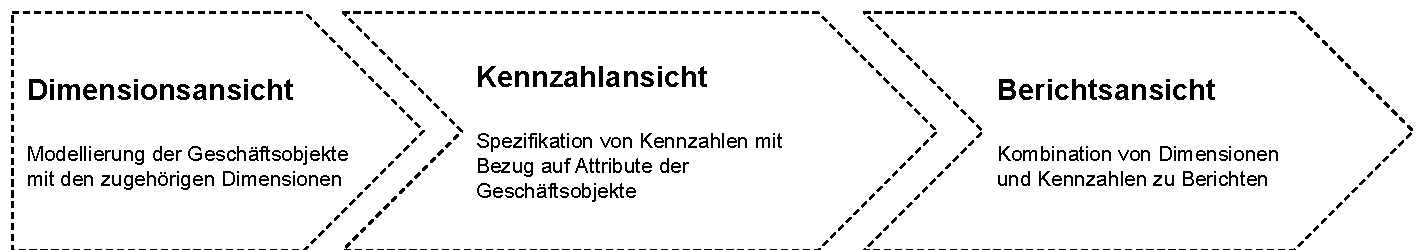
\includegraphics[scale=0.60]{content/figures/datafurnace-process}
    \caption{\textit{DataFurnace}-Prozess}\label{datafurnace-prozess}
  \end{figure}

  Der Wechsel zwischen der Dimensions-, Kennzahl- und Berichtsansicht gelingt
  über die Kopfleiste der \textit{DataFurnace}-Software, in welcher zu jeder
  Ansicht ein Link abgebildet ist. Neben dem Link ist des Weiteren jeweils ein
  individuelles Symbol abgebildet, welches in jeder Ansicht bei Referenzen auf
  den jeweiligen Typ Dimension, Kennzahl oder Bericht wieder verwendet wird.
  Diese konsistente Nutzung der Symbole durch die gesamte Oberfläche hindurch
  stützt sich auf die vierte \textit{Usability-Heuristic} von
  \textsc{\citeauthor{nielsen1994heuristic}} für Konsistenz und Standards und
  reduziert die nötige Denkleistung eines Nutzers bei der Bedienung der
  Software durch die bessere Wiedererkennbarkeit der
  Typen~(\citeyear{nielsen1994heuristic}, S. 30).  Die gleiche
  \textit{Usability-Heuristik} wird auch bei der Funktion zur Löschung von
  Objekten beachtet. In der gesamten Oberfläche kann ein Objekt durch einen
  Klick auf das \textit{Löschen}-Symbol, einem roten Papierkorb, entfernt
  werden, welches direkt auf dem zu löschenden Objekt abgebildet ist.


  \subsection{Dimensionsansicht}

  Die Modellierungsmethode beginnt in der Dimensionsansicht, welche sich aus
  Baumstrukturen zur Representation von Geschäftsobjekten mit ihren Attributen
  und Dimensionenauf der linken Seite und einer Detailansicht zur näheren
  Beschreibung einzelner Elemente auf der rechten Seite aufbaut. 

  Auf der linken Seite der Benutzeroberfläche fügt der Nutzer zunächst alle
  Geschäftsobjekte, zu denen er eine Analyse modellieren möchte, hinzu. Im
  oberen Teil des Geschäftsobjektkastens, welcher für jedes neues Geschäftsobjekt erscheint, kann
  der Name eines Geschäftsobjekts gesetzt und das gesamte Objekt gelöscht
  werden. Zum löschen des Geschäftsobjekts klickt ein Nutzer zunächst auf das
  \textit{Löschen}-Symbol in der oberen Leiste, wodurch ein Dialog zur
  Bestätigung geöffnet wird. Erst wenn der Nutzer diesen Dialog bestätigt, wird
  das Geschäftsobjekt mit all seinen Dimensionen, Dimensionsleveln und
  Attributen aus dem System gelöscht. Dieser Sicherheitsmechanismus folgt der
  fünften \textit{Usability-Heuristic} von
  \textsc{\citeauthor{nielsen1994heuristic}} zur Vorbeugung von schwerwiegenden
  Fehlern eines Nutzers~(\citeyear{nielsen1994heuristic}, S. 30).

  Im Geschäftsobjektkasten können des Weiteren Dimensionen dem Geschäftsobjekt
  hinzugefügt werden, welchen wiederum beliebig viele Dimensionslevel und
  schlussendlich ein Attribut untergeordnet werden kann. Für die weitere
  Erläuterung der Ansicht wird das Wort Element als Generalisierung von
  Dimension, Dimensionslevel und Attribut verwendet.  Einem
  Geschäftsobjekt können folglich beliebig viele Dimensionen angehören. Eine
  Dimension kann in beliebig viele Dimensionslevel aufgeteilt werden. Einem
  Dimensionslevel können weitere Dimensionslevel oder ein Attribut folgen. Eine
  Dimension-Dimensionslevel Kette muss mit einem Attribut enden. Einem Attribut
  können keine weiteren Elemente folgen. Ein Beispiel ist in
  Abbildung~\ref{fig:baumstruktur-produkt} zu sehen.

	\begin{figure}
		\footnotesize

		\begin{forest}
			for tree={grow'=0,
				child anchor=west,
				parent anchor=south,
				anchor=west,
				calign=first,
				edge path={\noexpand\path[draw, \forestoption{edge}]
					(!u.south west) + (7.5pt,0) |- node[fill,inner sep=1.25pt] {} (.child anchor)\forestoption{edge label};
				},
				before typesetting nodes={if n=1
						{insert before={[,phantom]}}
						{}
				},
				fit=band,
				before computing xy={l=15pt},
			}
		[Geschäftsobjekt \textit{Produkt}
			[Dimension \textit{Zeit}
				[Dimenionslevel \textit{Jahr}
					[\ldots{}
						[Attribut \textit{Verfallsdatum}]
					]
				]
			]
			[Dimension \textit{Ort}
				[\ldots{}]
			]
		]
		\end{forest}
    \caption{Baumstruktur des Geschäftsobjekts \textit{Produkt}}\label{fig:baumstruktur-produkt}
	\end{figure}

  Wird einer Dimension ein Dimensionslevel, einem Dimensionslevel ein weiteres
  Dimensionslevel oder einem Dimensionslevel ein Attribut untergeordnet, so
  erscheint dieses unterhalb des Elternelements, eingerückt wie in einer
  klassischen Ordnerbaumstruktur. Die Kindelemente eines Elternelements können
  auf- und zugeklappt, \bzw{} ein- und ausgeblendet werden, was es dem Nutzer
  ohne viel Aufwand ermöglicht, Teilausschnitte des Modells übersichtlich
  betrachten zu können, ohne diese in seperate Modelle exportieren zu
  müssen~\cite[][S. 6 f.]{fleischer2013konstruktion}. \todo{Zitat nochmal
  überprüfen. Ordentlich umschrieben?} Elemente können, durch einen klick auf
  das \textit{Löschen}-Symbol, gelöscht und, durch einen Klick auf den Namen, an
  der Stelle umbenannt werden.

  Neben der einfachen Charakterisierung von Elementen durch einen Namen,
  spezifiziert in der Baumstruktur auf der linken Seite der Dimensionsansicht,
  kann ein Nutzer auf der rechten Seite Details eines Elements einsehen und
  bearbeiten.  Hierzu wählt er in der Baumstruktur ein Element durch einen
  Klick aus, welches daraufhin auf der rechten Seite der Ansicht im Detail
  angezeigt wird. Im oberen Teil der Detailansicht ist zunächst der Name des
  Elements inklusive der Namen seiner Elternelemente als sogenannte
  \textit{Breadcrumb}-Navigation~\cite[][S. 1316]{maldonado2002common}
  angezeigt.  Der Name des Elements kann auch hier durch einen Klick auf das
  Wort an der Stelle bearbeitet werden. Sollen Details eines Elternobjekts
  bearbeitet werden genügt ein Klick auf den Namen des Elternelements in der
  \textit{Breadcrump}-Navigation, um zur Detailansicht des geforderten Elements
  zu wechseln. 

  Unterhalb dieser Hierarchienavigation findet sich der Typ des Elements.
  Möglichkeiten sind, zur Erinnerung: Dimension, Dimensionslevel und Attribut.
  Reicht der Name selbst nicht zur Beschreibung des Elements aus, kann
  unterhalb des Typ-Feldes eine Beschreibung in einem Freitextfeld spezifiziert
  werden. Für die spätere Modellierung von Filtern und Gruppen in Berichten
  können Dimensionsleveln und Attributen unterhalb der Beschreibung mögliche
  Ausprägungen hinzugefügt werden, welche in einer Liste erscheinen. Der Name
  einer Ausprägung kann durch einen Klick auf ebendiesen erneut verändert
  werden und die gesamte Ausprägung kann über das
  \textit{Löschen}-Symbol entfernt werden.

  Ihm Rahmen des Anwendungsfallbeispiels aus
  Abschnitt~\ref{sec:anwendungsfallbeispiel} würde ein Nutzer in der
  Dimensionsansicht die Geschäftsobjekte \textit{Produkt} und \textit{Kunde}
  mit ihren jeweiligen Attributen, Dimensionen, Dimensionsleveln und
  Dimensionslevelausprägungen modellieren. Besondere Beachtung bei der
  Modellierung des Geschäftsobjekts \textit{Produkt} sollten die Dimensionen
  der Attribute \textit{Warenlinie}, \textit{Verfallsdatum} und
  \textit{Standort} erhalten, um in der nachfolgenden Analyse nach der
  Dimensionslevelausprägung \textit{Lebensmittel} filtern und nach den
  Dimensionslevelausprägungen \textit{Oktober}, \textit{November} und
  \textit{Münster}, \textit{Bonn} gruppieren zu können. Für die Modellierung
  des Geschäftsobjekts \textit{Kunde} ist die Dimension \textit{Zeit} mit dem
  Dimensionslevel \textit{Jahr} für das Attribut \textit{ZuletztEingekauft}
  wichtig, um diejenigen Kunden ausfiltern zu können, welche in diesem Jahr
  noch nicht beim Unternehmen eingekauft haben.


  \subsection{Kennzahlansicht}

  Der zweite Schritt der \textit{DataFurnace}-Modellierungsmethode ist die
  Definition von Kennzahlen für die spätere Auswertung der
  Geschäftsobjektinstanzen, welche in der Kennzahlansicht vorgenommen werden
  kann. Wie auch die Dimensionsansicht teilt sie sich in zwei Spalten auf. Auf
  der linken Seite befindet sich eine Auflistung aller erstellten Kennzahlen.
  Durch einen Klick auf das Plus-Symbol in der oberen rechten Ecke können
  beliebig viele weitere Kennzahlen hinzugefügt werden, welche in ebendieser
  Liste neu erscheinen.

  Klickt ein Nutzer auf eine Kennzahl in der Liste auf der linken Seite der
  Ansicht, erscheint auf der rechten Seite der Kennzahleditor für die
  ausgewählte Kennzahl. Zunächst kann ein Nutzer den Namen der Kennzahl über
  einen Klick auf diesen in der oberen Leiste setzen. Außerdem kann er über das
  \textit{Löschen}-Symbol die Kennzahl aus dem System entfernen. In der unteren
  Leiste wird der Ausdruckkasten angezeigt. Mögliche Ausdrücke sind der
  \mbox{Attribut-,} \mbox{Konstanten-,} \mbox{Kennzahl-,} \mbox{Operator-,}
  Funktions- und Klammerausdruck.  Des Weiteren ist rechts neben dem
  Funktionsbaukasten die Funktion zur Löschung eines Ausdrucks gegeben.

  In der Mitte des Kennzahleditors wird die Formel zu Berechnung der Kennzahl
  angezeigt. Bei einer just erstellten Kennzahl wird hier lediglich der
  Kennzahlname visualisiert, gefolgt von einem Gleichheitszeichen. Das
  Gleichheitszeichen hält hier die Funktion einer Zuweisung wie im Gebrauch
  der Informatik, nicht eines Vergleichs wie in der Mathematik, inne.
  Alternativ könnte die Zuweisung an dieser Stelle auch durch das Zeichen
  \mbox{:=} verdeutlicht werden. 
  
  Eine Kennzahlformel in der \textit{DataFurnace}-Sprache besteht aus
  Ausdrücken, welche ein Nutzer über den Funktionsbaukasten in der unteren
  Leiste der Formel hinzufügen kann. Um an beliebigen Positionen der Formel
  Ausdrücke hinzufügen \bzw{} löschen zu können, kann mit Hilfe der Maus ein
  Cursor vor oder hinter jeden bestehenden Ausdruck gesetzt werden, welcher die
  aktuelle Position wie in einem Texteingabefeld markiert. Will ein Nutzer die
  Formel einer neu erstellten Kennzahl spezifizieren, klickt er zunächst hinter
  das Gleichheitszeichen um den Cursor zu positionieren.  Daraufhin wählt er
  aus dem Funktionsbaukasten beliebig viele Ausdrücke aus, welche in der
  gleichen Reihenfolge hinter dem gesetzten Cursor erscheinen.  Dieser springt
  nach dem Erscheinen eines Ausdrucks eine Stelle weiter nach rechts hinter den
  neu erstellten Ausdruck. 

  Um Fehler in der Kennzahlformel zu verhindern, werden dem Nutzer im
  Funktionsbaukasten immer nur die Ausdrücke zur Auswahl gestellt, welche nicht
  zu einer syntaktisch inkorrekten Formel führen, wenn man sie an der aktuellen
  Cursor-Position einfügt. Hat ein Nutzer beispielsweise in einer neuen
  Kennzahlformel bisher lediglich eine Konstante hinzugefügt und den Cursor
  hinter dieser belassen, so wird ihm im Formelbaukasten nun lediglich der
  Operatorausdruck zur Auswahl gestellt. Fügt der Nutzer diesen der Formel
  hinzu, werden ihm im nächsten Schritt alle Ausdrücke bis auf den
  Operatorausdruck im Funktionsbaukasten zur Verfügung gestellt. Diese
  intelligente Auswahl im Baukasten ist angelehnt an die fünfte
  \textit{Usability-Heuristic} von \textsc{\citeauthor{nielsen1994heuristic}},
  indem sie mögliches Fehlerverhalten des Nutzers
  verhindert~(\citeyear{nielsen1994heuristic}, S. 30).

  Viele Ausdrücke der \textit{DataFurnace}-Sprache sind durch das soeben
  beschriebene Hinzufügen noch nicht ausreichend konfiguriert. Hierzu zählt der
  Attributausdruck, der Konstantenausdruck, der Kennzahlausdruck, der
  Operatorausdruck und der Funktionsausdruck. 

  \begin{itemize} 
    \item Durch einen Klick auf einen \textbf{Attributausdruck} wird ein Auswahldialog
      angezeigt, welcher alle zuvor in der Dimensionsansicht modellierten
      Geschäftsobjektattribute dem Nutzer zur Auswahl stellt.  Nach der Auswahl
      eines Attributes wird dessen Name in der Formel als Platzhalter
      angezeigt. 
      
    \item  \textbf{Konstantenausdrücke} können in der Formel über ein
      Textfeld, welches durch einen Klick auf den Ausdruck erscheint,
      spezifiziert werden. Hier können sowohl konkrete Zahlenwerte wie auch
      Namen als Synonym genannt werden.

    \item Durch einen Klick auf einen \textbf{Kennzahlausdruck} wird ein
      Auswahldialog angezeigt wie auch beim Attributausdruck, welcher alle
      erstellten Kennzahlen im System bis auf die aktuelle zur Auswahl stellt.
      Ein Nutzer kann hiervon eine auswählen, dessen Namen als ebenfalls als
      Platzhalter in der Formel erscheint.  

    \item Wird ein \textbf{Operatorausdruck} zur Konfiguration ausgewählt,
      kann der Nutzer zwischen den Operatoren für die mathematischen
      Grundrechenarten Addition, Subtraktion, Multiplikation und Division
      wählen, welche nach der Auswahl mit ihrem mathematischen Symbol in der Formel
      repräsentiert werden.

    \item Zur Konfiguration eines \textbf{Funktionsausdrucks} werden dem Nutzer
      vordefinierte Funktionen, wie \zB{} die \textit{nicht-leer}-Funktion oder
      die \textit{enthält}-Funktion angezeigt und die Möglichkeit gegeben,
      eigene Funktionen zu benennen.
  \end{itemize}

  Macht ein Nutzer während der Konfiguration eines Ausdrucks einen Fehler oder
  möchte im Nachhinein etwas an dem Ausdruck ändern, so kann der
  Konfigurationsprozess auf den gleichen Weg jeder Zeit erneut gestartet werden.  Will ein
  Nutzer an spezifischen Positionen der Formel weitere Ausdrücke hinzufügen
  oder löschen, klickt er an die gewünschte Position und erstellt über den
  Funktionsbaukasten weitere Ausdrücke oder löscht den Ausdruck links vom Cursor
  mit einem Klick auf das \textit{Löschen}-Symbol rechts vom Funktionsbaukasten
  in der unteren Leiste.

  Führt der Nutzer im Zuge des Anwendungsfallbeispiels aus
  Abschnitt~\ref{sec:anwendungsfallbeispiel} in der Kennzahlansicht die
  Modellierung fort, würde er zunächst mit der Spezifikation einer Kennzahl
  beginnen, welche die Validität des Attributes \textit{Verkaufspreis} des
  Geschäftsobjekts \textit{Produkt} überprüft. Es ist anzunehmen, dass eine
  Ausprägung des Attributs \textit{Verkaufspreis} dann valide ist, wenn sie
  sowohl nicht leer, als auch keine Buchstaben enthält. Der Nutzer erstellt
  zunächst eine neue Kennzahl. Im Formeleditor der Kennzahl fügt er die Formel
  \texttt{AND (NOT (ISEMPTY (Verkaufspreis)), NOT (CONTAINS (Verkaufspreis,
  [A\textminus{}Za\textminus{}z])))} ein, welche nur den boolschen Wert
  \textit{wahr} zurück gibt, wenn der \textit{Verkaufspreis} nicht leer ist und
  keine Buchstaben enthält. Analog zu dieser Kennzahl erstellt er ebenfalls
  Kennzahlenn für die Prüfung der Attribute \textit{E-Mail-Adresse} und
  \textit{Anschrift} des Geschäftsobjekts \textit{Kunde}.

  Neben den drei soeben beschriebenen Datenqualitätskennzahlen der Attribute
  \textit{Verkaufspreis}, \textit{E-Mail-Adresse} und \textit{Anschrift} wird
  noch die betriebswirtschaftliche Kennzahl \textit{Gewinn} benötigt, um in der
  späteren Analyse den Gewinnverlust durch abgelaufene Lebensmittel zwischen
  den Standort-Monat-Kombinationen vergleichen zu können. Hierzu erstellt der
  Nutzer wiederum eine neue Kennzahl mit der Formel \texttt{Verkaufspreis \textminus{}
  Einkaufspreis}.


  \subsection{Berichtsansicht}

  Im letzten Schritt der \textit{DataFurnace}-Modellierungsmethode werden
  Dimensionsspezifikationen und Kennzahldefinitionen zu Berichtsmodellen in der
  Berichtsansicht kombiniert. Die Struktur der Berichtsansicht teilt sich in
  drei Komponenten auf. Auf der linken Seite werden alle Geschäftsobjekte mit
  ihren zugehörigen Dimensionen, Dimensionsleveln und Attributen in der
  bereits bekannten Baumstruktur in der Geschäftsobjektkomponente abgebildet.
  Auf der rechten Seite werden alle Kennzahlen in der Kennzahlkomponente
  aufgelistet. In der Mitte befindet sich die Berichtskomponente, unterteilt in
  einen Abschnitt zur Filterung und der finalen Berichtstabelle.

  Sowohl die Geschäftsobjektkomponente auf der linken, als auch die
  Kennzahlkomponente auf der rechten Seite der Berichtsansicht sind übernommen
  aus den jeweils linken Seiten der Dimensions- und Kennzahlansicht, jedoch
  lediglich als anzeigende Komponente ohne Funktionalität zur Erstellung,
  Bearbeitung oder Löschung ihrer Elemente. Sie dienen, wie der
  Funktionsbaukasten in der Kennzahlansicht, als Quelle für Dimensionslevel,
  Attribute und Kennzahlen in der Modellierung von Berichten. Wie auch in der
  Dimensionsansicht können die Geschäftsobjektbaumstrukturen auf der linken
  Seite der Berichtsansicht weiterhin durch auf- und zuklappen traversiert
  werden.

  In der Mitte der Berichtsansicht befindet sich die Kernkomponente für die
  Berichtsmodellierung. Zunächst muss ein neuer Bericht
  in der Komponente erstellt werden, welcher sich wiederum über das
  \textit{Löschen}-Symbol entfernen und in der oberen Leiste durch einen Klick
  auf den Namen benennen lässt. Die Komponente unterteilt sich horizontal in
  den tabellarischen Bericht (Tabellenkomponente) und den spezifizierten
  Filtern (Filterkomponente) darunter. Zunächst soll auf die
  Filterspezifikation eingegangenn werden. 
  
  \paragraph{Filterkomponente}
  
  Wie in Abschnitt~\ref{paragraph:filternde-komponente}
  beschrieben, kann ein Filter sowohl auf einem Dimensionslevel als auch einer
  Kennzahl basieren. Will ein Nutzer eine neue Kennzahl auf Basis eines
  Dimensionslevels erstellen, sucht er das Level zunächst aus den
  Geschäftsobjektbaumstrukturen auf der linken Seite der Berichtsansicht heraus
  und zieht es mit der Maus aus der Geschäftsobjektkomponente in die
  Filterkomponente der Ansicht. Sobald er das Dimensionslevel in der Komponente
  ablegt, wird ein neuer Filter erstellt. In dem Filter werden alle
  Dimensionslevelausprägungen aufgelistet, welche im ersten Schritt der
  \textit{DataFurnace}-Modellierungsmethode für das Dimensionslevel
  spezifiziert wurden. Nun kann der Nutzer anhand einer Positivliste
  diejenigen Ausprägungen auswählen, nach welchen er die gesamte
  Geschäftsobjektinstanzmenge filtern möchte.

  Möchte der Nutzer auf Basis einer Kennzahl filtern, zieht er analog zur
  Basis auf ein Dimensionslevel, eine Kennzahl aus der rechten
  Kennzahlkomponente und legt diese in der Filterkomponente ab. Sobald die
  Kennzahl über der Filterkomponente los gelassen wird, wird ein Filter auf
  Basis der Kennzahl erstellt. Nun kann der Nutzer im Filter spezifizieren, bei
  welchen Ergebnissen der Kennzahl er ausfiltern möchte und bei welchen
  Ergebnissen eine Geschäftsobjektinstanz in die nähere Auswahl weiter kommt,
  indem er \zB{} Ober- und Untergrenzen bei Kennzahlen mit
  Zahlenwertergebnissen definiert, oder bei Kennzahlen mit booleschen
  Rückgabewerten entscheidet, ob Geschäftsobjektinstanzen die Prüfung der
  Kennzahl bestehen müssen oder nicht bestehen dürfen.

  Wird ein Filter nicht mehr benötigt, kann dieser über das
  \textit{Löschen}-Symbol am rechten Rand des Filters gelöscht werden. Die
  Dimensionslevel- oder Kennzahlbasis eines Filters ist in der Gesamtmenge
  aller spezifizierten Filter einzigartig. Die gleiche Basis kann nicht in
  mehreren Filtern eines Berichts vorkommen.

  \paragraph{Tabellenkomponente}

  Die Tabellenkomponente der Berichtsansicht der \textit{DataFurnace}-Software
  ermöglicht es, Berichtstabellen der \textit{DataFurnace}-Sprache zu
  modellieren. Die Modellierung lässt sich in zwei Gruppen unterteilen: in die
  Modellierung der Tabellenkopfzeilen mit Dimensionsleveln und in die
  Modellierung der Tabellenkopfspalte mit Kennzahlen.

  Wie in Abschnitt~\ref{paragraph:tabellenkomponente} beschrieben,
  spezifizieren die Tabellenkopfzeilen mit Hilfe von Dimensionsleveln, welche
  Unternehmensdaten in der Analyse betrachtet werden und wie die Daten
  gruppiert werden. Hierzu wählt ein Nutzer zunächst die Dimensionslevel für
  die Tabelle aus, indem er sie in den Geschäftsobjektbaumstrukturen auf der
  linken Seite der Berichtsansicht ausfindig macht und sie auf die Tabelle
  zieht. Sobald ein Dimensionslevel auf der Tabelle abgesetzt wurde, wird eine
  neue Tabellenkopfzeile auf Basis dieses Dimensionslevels erstellt. Dieser
  Vorgang kann mit beliebig vielen Dimensionsleveln wiederholt werden, jedoch
  kann ein Dimensionslevel nicht mehrfach einer Tabelle hinzugefügt werden. Die
  erste Zelle einer neu erstellten Tabellenkopfzeile enthält den Namen des
  Dimensionslevels, auf dessen Basis die Zeile beruht. Des Weiteren wird der
  Tabellenkopfzeile pro verfügbarer Ausprägung des Dimensionslevels eine Zelle
  mit dem Namen des Dimensionslevels hinzugefügt.

  Sollen nicht alle Ausprägungen eines Dimensionslevels in der Tabelle des
  Berichts betrachtet werden, können einzelne Ausprägungen abgewählt werden.
  Hierzu wird zunächst der Ausprägungsauswahldialog über das
  \textit{Filter}-Symbol links neben dem Namen des Dimensionslevels geöffnet.
  In diesem können ausgewählte Dimensionslevelausprägungen abgewählt und abgewählte
  Dimensionslevel ausgewählt werden. Die Tabelle passt sich in Echtzeit an die
  vorgenommenen Änderungen an, indem sie die Anzahl der Zellen der aktuellen
  Tabellenkopfspalte um die Ausprägung erweitert respektive kürzt und alle
  Ausprägungskombinationen der darunterliegenden Tabellenkopfzeilen in
  Abhängigkeit der Änderungen entsprechend korrigiert. Als Beispiel dienen hier
  Tabelle~\ref{table:berichtstabellenkopf20142015}
  und~\ref{table:berichtstabellenkopf201420152016}, welche die Tabellenkopfspalte
  ohne und mit der Dimensionslevelausprägung \textit{2016} des Dimensionslevels
  \textit{Jahr} abbilden. Hier gilt es die Änderungen in der Zeile
  \textit{Bundesland} zu betrachten.

    \begin{table}[]
      \footnotesize
      \begin{tabular}{c c c c c c c c c}
        \textbf{Warenlinie} & \multicolumn{4}{c}{Bürobedarf} & \multicolumn{4}{c}{Lebensmittel} \\
            \cmidrule(lr){2-5}\cmidrule(lr){6-9}
        \textbf{Jahr} & \multicolumn{2}{c}{2014} & \multicolumn{2}{c}{2015} & \multicolumn{2}{c}{2014} & \multicolumn{2}{c}{2015}\\
            \cmidrule(lr){2-3}\cmidrule(lr){4-5}\cmidrule(lr){6-7}\cmidrule(lr){8-9}
        \textbf{Bundesland} & NRW & HH & NRW & HH & NRW & HH & NRW & HH \\
      \end{tabular}
      \caption{Beispiel der Tabellenkopfzeilen mit den Ausprägungen \textit{2014} und \textit{2015}}\label{table:berichtstabellenkopf20142015}
    \end{table}

    \begin{table}
      \footnotesize
      \begin{tabular}{c c c c c c c c c c c c c}
        \textbf{Warenlinie} & \multicolumn{6}{c}{Bürobedarf} & \multicolumn{6}{c}{Lebensmittel} \\
            \cmidrule(lr){2-7}\cmidrule(lr){8-13}
        \textbf{Jahr} & \multicolumn{2}{c}{2014} & \multicolumn{2}{c}{2015} & \multicolumn{2}{c}{2016} & \multicolumn{2}{c}{2014} & \multicolumn{2}{c}{2015} & \multicolumn{2}{c}{2016}\\
            \cmidrule(lr){2-3}\cmidrule(lr){4-5}\cmidrule(lr){6-7}\cmidrule(lr){8-9}\cmidrule(lr){10-11}\cmidrule(lr){12-13}
        \textbf{Bundesland} & NRW & HH & NRW & HH & NRW & HH & NRW & HH & NRW & HH & NRW & HH \\
      \end{tabular}
      \caption{Beispiel der Tabellenkopfzeilen mit den Ausprägungen \textit{2014}, \textit{2015} und \textit{2016}}\label{table:berichtstabellenkopf201420152016}
    \end{table}

  In Abschnitt~\ref{paragraph:tabellenkomponente} wurde festgestellt, dass die
  Auftrittsreihenfolge der Tabellenkopfzeilen für die Übersichtlichtkeit der
  Tabelle relevant sind, weswegen die \textit{DataFurnace}-Software eine Anpassung
  dieser ermöglicht. Hierzu zieht ein Nutzer die zu
  verschiebende Zeile an ihre neue Position. Die
  Dimensionslevelausprägungskombinationen werden automatisch ensprechend
  angepasst. Soll eine Tabellenkopfzeile nicht verschoben, sondern gänzlich aus
  der Tabelle entfernt werden, kann dies über einen Klick auf das
  \textit{Löschen}-Symbol rechts neben dem Dimensionslevelnamen in der ersten
  Zelle der Zeile realisiert werden.

  Die Spezifikation von Kennzahlen in der Berichtstabelle wird in der
  Tabellenkopfspalte realisiert. Analog zu den Tabellenkopfzeilen kann eine
  Kennzahl der Tabellenkopfspalte hinzugefügt werden, indem sie aus der rechten
  Kennzahlkomponente auf die Berichtstabelle herüber gezogen wird. Wird die
  Kennzahl über der Berichtstabelle losgelassen, erstellt die
  \textit{DataFurnace}-Software in der Spalte eine neue Zelle mit dem Namen der
  Kennzahl. Wurde eine Kennzahl versehentlich hinzugefügt oder in der
  Berichtstabelle nicht weiter benötigt kann sie über das
  \textit{Löschen}-Symbol entfernt werden.

  Die Modellierung im Rahmen des Anwendungsfallbeispiels aus
  Abschnitt~\ref{sec:anwendungsfallbeispiel} wird in der Berichtsansicht
  abgeschlossen. Zunächst erstellt ein Nutzer für die Analyse des
  Geschäftsobjekts \textit{Produkt} einen neuen Bericht. Die Marketingkampagne
  ist auf Lebensmittel fokussiert. Folglich wird dem Bericht ein Filter auf
  Basis des Dimensionslevels \textit{Warenlinie} hinzugefügt und in der
  Positivliste lediglich die Dimensionslevelausprägung \textit{Lebensmittel}
  ausgewählt. Des Weiteren fügt der Nutzer auf Basis der
  Preisvalidationskennzahl des Attributes \textit{Verkaufspreis} einen weiteren
  Filter hinzu. Dieser hat zur Folge, dass in der Tabelle nur die
  \textit{Produkt}-Geschäftsobjektinstanzen betrachtet werden, welche einen
  validen Preis haben. Nun soll im Anwendungsfallbeispiel der Gewinnverlust der
  Standorte \textit{Münster} und \textit{Bonn} in den Monaten \textit{Oktober}
  und \textit{November} verglichen werden. Um dies zu realisieren fügt der
  Nutzer die Dimensionslevel \textit{Ort} und \textit{Monat} den
  Tabellenkopfzeilen hinzu und wählt die Dimensionslevelausprägungen
  \textit{Münster} und \textit{Bonn} und \textit{Oktober} und \textit{November}
  aus. Abschließend fügt er die Kennzahl zur Berechnung des \textit{Gewinns}
  der Tabellenkopfspalte hinzu.  \todo[inline]{Beispielberichtstabelle}

  Für die Analyse des Geschäftsobjekts \textit{Kunde} fügt der Nutzer einen
  weiteren Bericht hinzu. In diesem Bericht erstellt er einen Filter auf Basis
  des Dimensionslevels Jahr des Attributes \textit{ZuletztEingekauft} und fügt
  die Dimensionslevelausprägung \textit{2016} der Positivliste des Filters
  hinzu. Somit werden alle Kunden in der weiteren Analyse ausgefiltert, welche
  in diesem Jahr noch nicht beim Unternehmen eingekauft haben. Um die Anzahl
  hinterlegter \textit{E-Mail-Adressen} mit der Anzahl hinterlegter
  \textit{Postanschriften} zu vergleichen, werden die zuvor erstellten
  Kennzahlen der Attribute \textit{E-Mail-Adresse} und \textit{Anschrift} der
  Tabellenkopfspalte hinzugefügt. Zuletzt wird der Bericht durch ein beliebiges
  Dimensionslevel als Platzhalter für das Geschäftsobjekt \textit{Kunde} in den
  Tabellenkopfzeilen erweitert.


  \section{Technische Umsetzung}

  \todo[inline]{Technische Umsetzung ca.\ 1--2 Seiten, \ggf{} bis zu fünf Seiten}
  \todo[inline]{Sollen alle Technologien mit einer Fußnote mit der Website ausgestattet werden?}

  Die \textit{DataFurnace}-Software ist eine moderne Applikation, welche sich
  innovativer Technologien des neuesten Standes der Informationstechnik
  bedient. Eine nähere Erläuterung jeder Technologie und deren
  Integration in dem Softwaresystem würde über den Rahmen dieser Arbeit hinaus
  gehen, jedoch soll im Folgenden auf die Systemarchitektur inklusive
  einzelner Entscheidungserläuterungen und den Entwicklungsprozess kurz
  eingegangen werden.\todo{Entwicklungsprozess streichen?}


  \paragraph{Systemarchitektur}
  Die \textit{DataFurnace}-Software ist eine eigenständige  Webanwendung,
  welche auf dem hierfür klassischem Client-Sever-Modell aufbaut. Die
  Serverarchitektur setzt sich aus einem Webserver und einem Datenbankserver
  zusammen. Der Webserver ist eine \textit{NodeJS}-Anwendung unter Verwendung
  des \textit{MeteorJS}-Frameworks. Über das \textit{HTTP}-Protokoll für
  Anzeige- und Anwendungslogik und das \textit{DDP}-Protokoll für
  Anwendungsdaten kommuniziert er mit dem Client. Neben der Verbindung zum
  Client hat der Anwendungsserver direkten Zugriff auf den Datenbankserver.
  Bedingt durch die Einschränkung, dass \textit{MeteorJS} seine volle
  Funktionalität nur in Verbindung mit einem \textit{MongoDB}-Datenbankservers
  bieten kann, wird ebendiese Technologie für den Datenbankserver der
  \textit{DataFurnace}-Software eingesetzt. Sowohl Webserver als auch
  Datenbankserver werden mit der Virtualisierungssoftware \textit{Docker}
  isoliert in Containern betrieben.  Der Client der
  \textit{DataFurnace}-Software kann mit Hilfe eines Webbrowsers aufgerufen
  werden. Für das Frontend der Applikation wird die
  \textit{Javascript}-Bibliothek \textit{ReactJS} in Kombination mit der
  Anzeigebibliothek \textit{React-Bootstrap} und dem Programmpaket
  \textit{React-Router} für das \textit{URI}-Routen-Management verwendet.  Der
  gesamte Aufbau der Architektur wird durch
  Abbildung~\ref{fig:systemarchitektur} erneut verdeutlicht.

  \begin{figure}
		\footnotesize
    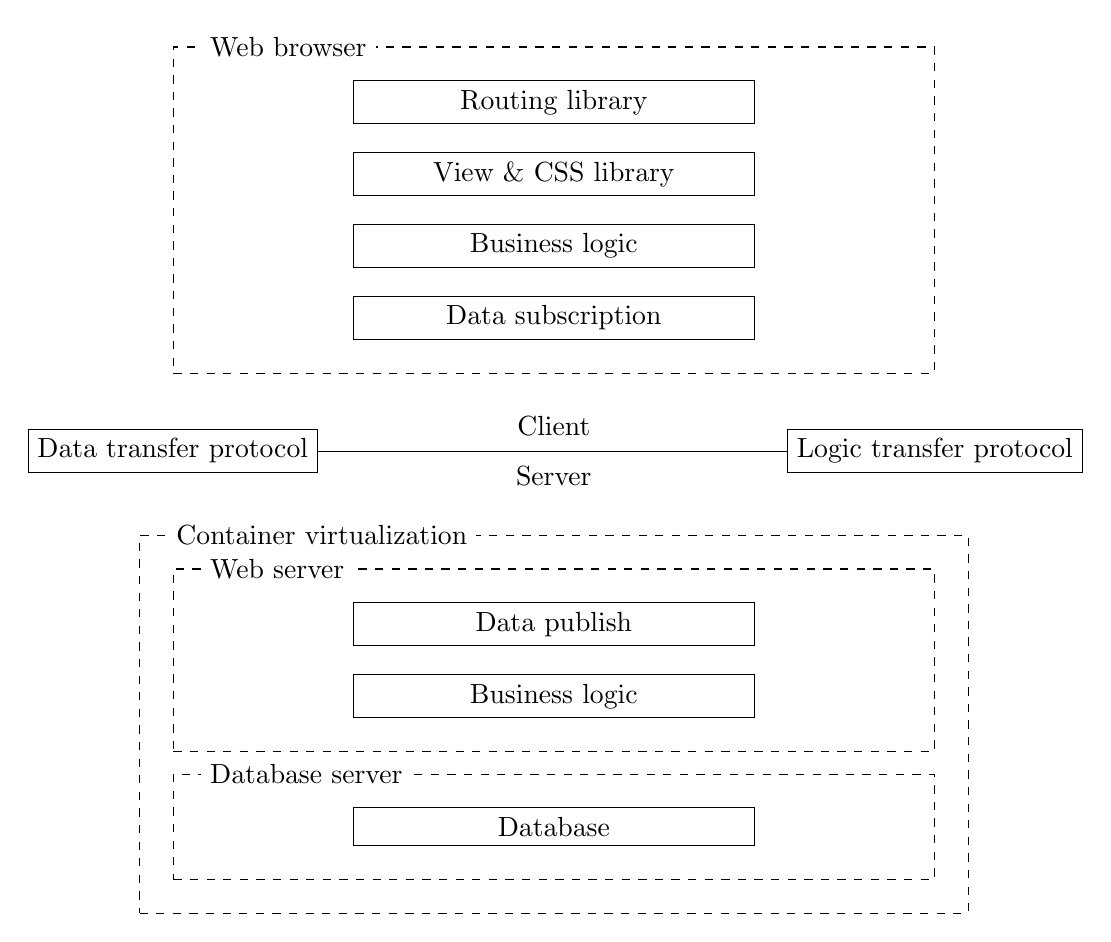
\begin{tikzpicture}[]
      \tikzstyle{container} =  [dashed, draw, minimum width=\textwidth - 70pt, inner sep=12pt]
      \tikzstyle{box} =  [draw, minimum width=\textwidth - 200pt]

      \node (publish) [box] {Data publish};
      \node (businessLogic) [box, below = 10pt of publish] {Business logic};

      \node (nodeJS) [container, fit= (publish) (businessLogic)] {};
      \node [fill=white, right=10pt] at (nodeJS.north west) {Web server};

      \node (mongoDB) [box, draw, below = 20pt of nodeJS] {Database};

      \node (databaseserver) [container, fit=(mongoDB)] {};
      \node [fill=white, right=10pt] at (databaseserver.north west) {Database server};

      \node (docker) [container, fit= (nodeJS) (databaseserver)] {};
      \node[fill=white, right=10pt] at (docker.north west) {Container virtualization};

      \node (line) [draw, minimum height=0pt, minimum width=\textwidth - 70pt, inner sep=0pt, above = 30pt of docker] {};

      \node [above=2pt] at (line.north) {Client};
      \node [below=2pt] at (line.south) {Server};
      \node [fill=white, draw] at (line.north west) {Data transfer protocol};
      \node [fill=white, draw] at (line.north east) {Logic transfer protocol};

      \node (subscribe) [box, above=40pt of line] {Data subscription};
      \node (businessLogicClient) [box, above= 10pt of subscribe] {Business logic};
      \node (reactJS) [box, above= 10pt of businessLogicClient] {View \& CSS library};
      \node (router) [box, above=10pt of reactJS] {Routing library};

      \node (webbrowser) [container, fit= (subscribe) (businessLogicClient) (reactJS) (router)]{};
      \node[fill=white, right=10pt] at (webbrowser.north west) {Web browser};
    \end{tikzpicture}
    \caption{Systemarchitektur der \textit{DataFurnace}-Software}\label{fig:systemarchitektur}
	\end{figure}

  Mit dieser Systemarchitektur kann die \textit{DataFurnace}-Software losgelöst
  von \textit{DataRocket} eigenständig betrieben und genutzt werden. Neben der
  Eigenständigkeit der Software ist auch die Integrierbarkeit in
  \textit{DataRocket} gefordert. Sowohl \textit{DataRocket} als auch die
  \textit{DataFurnace}-Software sind server- und clientseitig in der
  Programmiersprache \textit{JavaScript} geschrieben, des Weiteren nutzen beide
  das \textit{MeteorJS}-Framework, womit die Integration der serverseitigen
  Funktionalität leicht umzusetzen ist. Clientseitig setzt \textit{DataRocket}
  auf die Oberflächenbibliothek \textit{Blaze}, \textit{DataFurnace} setzt den
  Konkurrenten \textit{ReactJS} ein. Beide sind jedoch insofern kompatibel, als
  dass einzelne \textit{ReactJS}-Komponenten mit Hilfe einer kleinen
  Hilfsbibliothek in \textit{Blaze}-Komponenten integriert werden können.


  % \paragraph{Publish und Subscribe}
  % Designpattern


  \paragraph{Echtzeitkollaboration}

  Wie in der Anforderungsanalyse der \textit{DataFurnace}-Software,
  Abschnitt~\ref{sec:software/anforderungsanalyse} beschrieben, soll die
  Software von mehreren Personen gleichzeitig genutzt werden können. Um diese
  Kollaboration über mehrere Clients hinweg so benutzerfreundlich wie möglich
  zu gestalten, müssen Änderungen eines Nutzers in Echtzeit nicht nur im
  eigenen Client, sondern allen Clients sichtbar sein. Um diese Reaktivität
  technisch umsetzen zu können, werden das Webserver-Framework \textit{MeteorJS},
  die Datenbank \textit{MongoDB}, sowie die \textit{JavaScript}-Bibliothek
  \textit{ReactJS} verwendet. Anhand eines konkreten Beispiels soll im
  Folgenden das Zusammenspiel dieser Technologien erläutert werden. 
  
  Klickt Nutzer A in der Dimensionsansicht auf das \textit{Löschen}-Symbol
  eines Geschäftsobjekts, wird von dem \textit{JavaScript}-Framework
  \textit{ReactJS} eine Funktion ausgeführt, welche das Geschäftsobjekt aus dem
  lokalen Speicher löscht. Wird der lokale Speicher geändert, reagiert
  \textit{ReactJS} darauf, indem es die aktuelle Oberfläche im Hintergrund neu
  berechnet und das Delta aus aktueller und neuer Oberfläche in der aktuellen
  anpasst. Während \textit{ReactJS} die Oberfläche ändert, reagiert auch das
  \textit{Meteor}-Framework, indem es die Änderungen auch auf den
  Serverspeicher, alias die \textit{MongoDB}, anwendet. Wird etwas an dem
  Zustand der \textit{MongoDB} geändert, so werden diese Änderungen automatisch
  von Meteor an alle Clients verteilt. Somit wird auch der lokale Speicher von
  Client B automatisch angepasst, was wiederum zur Folge hat, dass das
  \textit{ReactJS}-Framework die Oberfläche des Clients B neu berechnet und
  anzeigt, womit auch hier das Geschäftsobjekt gelöscht wird.

  % \todo[inline]{Dieser Abschnitt muss nicht-funktionales Ziel `Eigenständige
  % Software integrierbar in DataRocket' und `Echtzeitkollaboration' beantworten}
  % Falls auf React eingegangen wird, auch die Wiederverwendbarkeit einzelner Komponenten beschreiben.

%  \paragraph{React-Router}
%  \todo[inline]{React router Lade-Symbol für Usability Heuristic 1 `Visibility of system status'}

%  \paragraph{Entwicklungsprozess} Um eine hohe Softwarequalität sicher zu
%  stellen, wurde die \textit{DataFurnace}-Software angelehnt an dem
%  \textit{GitFlow}-Prinzip mit einer hohen Testabdeckung entwickelt.
%  
%  \begin{itemize}
%    \item GitFlow
%    \item Continuous Integration
%    \item Travis CI
%    \item Continuous Deployment
%    \item Digital Ocean
%    \item Docker
%    \item Mocha
%    \item Chai
%    \item Enzyme
%  \end{itemize}


% ################################################################################
\chapter{Evaluation}\label{ch:evaluation}

Um die Verständlichkeit und Anwendbarkeit der \textit{DataFurnace}-Sprache und
-Software zu prüfen, wurden 15 Kandidaten darum gebeten, die Datenanalyse des
Anwendungsfallbeispiels aus Abschnitt~\ref{sec:anwendungsfallbeispiel} in der
\textit{DataFurnace}-Software zu modellieren. Hierzu bekahmen sie eine kurze
Einweisung in die mutlidimensionale Modellierung
(Abschnitt~\ref{subsec:multidimensionale-modellierung}), \textit{DataRocket}
(Abschnitt~\ref{sec:Vorstellung-DataRocket}) und die
\textit{DataFurnace}-Sprache
(Abschnitt~\ref{ch:entwicklung-datafurnace-sprache}). Erklärungen zu der
\textit{DataFurnace}-Software wurden nicht im vorhinein gegeben.  In
Tabelle~\ref{table:befragungsgruppe} werden die ausgewählten Befragten näher
beschrieben.

  \begin{table}[]
    \footnotesize
    \begin{tabular}{c c c c}
      Beschäftigung & Technische Kentnisse & Geschlecht & Alter \\
      \toprule
      WI-Studentin & Intermediate & weiblich & 25 \\
      WI-Student & Intermediate & männlich & 23 \\
    \end{tabular}
    \caption{Befragungsgruppe}\label{table:befragungsgruppe}
  \end{table}

\todo[inline]{Alternativ der Begriff Beurteilung als Kapiteltitel}
\texthl{Wie finden andere das Tool, Feedback dokumentieren, gegebenenfalls mit Fragebogen}
 \paragraph{Integration in \textit{Datarocket}}
 Wenn nicht alle Dimensionslevel einer Dimension aus dem gleichen Attribut
 Informationen bekommen zum Beispiel in dem Fall, dass Jahr und Monat in zwei
 unterschiedlichen Attributen festgehalten sind, so kann dies im Dimensionsbaum
 spezifiziert werden, indem ihm mehrere Attribute hinzugefügt werden.

  \begin{figure}
    \resizebox{\columnwidth}{!}{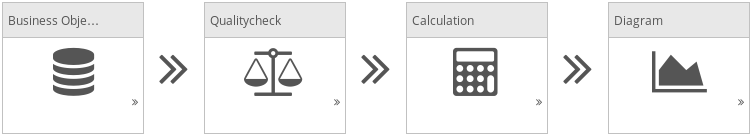
\includegraphics{content/figures/pipeline-bricks.png}}
    \caption{\textit{DataRockets} \textit{Datapipeline}-Bausteine}\label{}
  \end{figure}

	Ideen für die Zukunft
	\begin{itemize}
    \item Tastaturunterstützung im Formeleditor (Nielsen Nummer 7 `Flexibility
      and efficiency of use')
    \item Support Undo redo (Nielsen Nummer 3 `user control and freedom')
	\end{itemize}
% ################################################################################

% ################################################################################
\chapter{Fazit}\label{ch:fazit}
% ################################################################################
\todo[inline]{Fazit ca.\ 1--2 Seiten}



 % ################################################################################
  \chapter{notes}
\section{}
\begin{itemize}
  \item Beispieldatenbank AdventureWorks-Datenbank von Microsoft
\end{itemize}

\section{Aufteilung}
Am meisten soll \textit{inoscale Sprache und Methode} und \textit{DataFurnace} einnehmen. \textit{Existierende Methoden und Sprachen} soll nur einen kleinen Teil (max 3 Seiten) einnehmen.


\section{Offene Fragen}
\begin{itemize}
  \item Titel besprechen
  \item Struktur / Inhaltsverzeichnis besprechen
  \item Wie sehr soll welcher Teil der Arbeit gewichtet werden (Konkret in Seitenzahlen)
  \item Zeitplan Jetzt anmelden?
  \item Wie kann ich aus einem SQL-Schema eine Bezugsobjekt-Struktur generieren?
\end{itemize}

  % ################################################################################

\end{content}



% ################################################################################
% Appendix
% ################################################################################
%\begin{appendix}
%  \section{Some Appendix Section}\label{sec:appendix01}
Appendices provide only two structural levels, \viz, \texttt{\textbackslash{} section}, and \texttt{\textbackslash{} subsection}.

The numbering of figures, listings, tables, and footnotes is not reset. Thus, it continues as usual in the appendix.

\subsection{Some Appendix Subsection}

\lipsum[10]

%\end{appendix}



% ################################################################################
% References
% ################################################################################
\references{lib/library}



% ################################################################################
% Declaration of authorship
% ################################################################################
%\authorshipstatement[pagenumbering=false]
%\authorshipstatement[pagenumbering=true]
% \authorshipstatement[pagenumbering=only]

% Bonus: Wordcount
% cd %FOLDER WHERE THE .tex FILES ARE IN %
% clear
% texcount -total -q -col -sum *.tex

\end{document}
